% Options for packages loaded elsewhere
\PassOptionsToPackage{unicode}{hyperref}
\PassOptionsToPackage{hyphens}{url}
%
\documentclass[
]{book}
\usepackage{amsmath,amssymb}
\usepackage{iftex}
\ifPDFTeX
  \usepackage[T1]{fontenc}
  \usepackage[utf8]{inputenc}
  \usepackage{textcomp} % provide euro and other symbols
\else % if luatex or xetex
  \usepackage{unicode-math} % this also loads fontspec
  \defaultfontfeatures{Scale=MatchLowercase}
  \defaultfontfeatures[\rmfamily]{Ligatures=TeX,Scale=1}
\fi
\usepackage{lmodern}
\ifPDFTeX\else
  % xetex/luatex font selection
\fi
% Use upquote if available, for straight quotes in verbatim environments
\IfFileExists{upquote.sty}{\usepackage{upquote}}{}
\IfFileExists{microtype.sty}{% use microtype if available
  \usepackage[]{microtype}
  \UseMicrotypeSet[protrusion]{basicmath} % disable protrusion for tt fonts
}{}
\makeatletter
\@ifundefined{KOMAClassName}{% if non-KOMA class
  \IfFileExists{parskip.sty}{%
    \usepackage{parskip}
  }{% else
    \setlength{\parindent}{0pt}
    \setlength{\parskip}{6pt plus 2pt minus 1pt}}
}{% if KOMA class
  \KOMAoptions{parskip=half}}
\makeatother
\usepackage{xcolor}
\usepackage{color}
\usepackage{fancyvrb}
\newcommand{\VerbBar}{|}
\newcommand{\VERB}{\Verb[commandchars=\\\{\}]}
\DefineVerbatimEnvironment{Highlighting}{Verbatim}{commandchars=\\\{\}}
% Add ',fontsize=\small' for more characters per line
\usepackage{framed}
\definecolor{shadecolor}{RGB}{248,248,248}
\newenvironment{Shaded}{\begin{snugshade}}{\end{snugshade}}
\newcommand{\AlertTok}[1]{\textcolor[rgb]{0.94,0.16,0.16}{#1}}
\newcommand{\AnnotationTok}[1]{\textcolor[rgb]{0.56,0.35,0.01}{\textbf{\textit{#1}}}}
\newcommand{\AttributeTok}[1]{\textcolor[rgb]{0.13,0.29,0.53}{#1}}
\newcommand{\BaseNTok}[1]{\textcolor[rgb]{0.00,0.00,0.81}{#1}}
\newcommand{\BuiltInTok}[1]{#1}
\newcommand{\CharTok}[1]{\textcolor[rgb]{0.31,0.60,0.02}{#1}}
\newcommand{\CommentTok}[1]{\textcolor[rgb]{0.56,0.35,0.01}{\textit{#1}}}
\newcommand{\CommentVarTok}[1]{\textcolor[rgb]{0.56,0.35,0.01}{\textbf{\textit{#1}}}}
\newcommand{\ConstantTok}[1]{\textcolor[rgb]{0.56,0.35,0.01}{#1}}
\newcommand{\ControlFlowTok}[1]{\textcolor[rgb]{0.13,0.29,0.53}{\textbf{#1}}}
\newcommand{\DataTypeTok}[1]{\textcolor[rgb]{0.13,0.29,0.53}{#1}}
\newcommand{\DecValTok}[1]{\textcolor[rgb]{0.00,0.00,0.81}{#1}}
\newcommand{\DocumentationTok}[1]{\textcolor[rgb]{0.56,0.35,0.01}{\textbf{\textit{#1}}}}
\newcommand{\ErrorTok}[1]{\textcolor[rgb]{0.64,0.00,0.00}{\textbf{#1}}}
\newcommand{\ExtensionTok}[1]{#1}
\newcommand{\FloatTok}[1]{\textcolor[rgb]{0.00,0.00,0.81}{#1}}
\newcommand{\FunctionTok}[1]{\textcolor[rgb]{0.13,0.29,0.53}{\textbf{#1}}}
\newcommand{\ImportTok}[1]{#1}
\newcommand{\InformationTok}[1]{\textcolor[rgb]{0.56,0.35,0.01}{\textbf{\textit{#1}}}}
\newcommand{\KeywordTok}[1]{\textcolor[rgb]{0.13,0.29,0.53}{\textbf{#1}}}
\newcommand{\NormalTok}[1]{#1}
\newcommand{\OperatorTok}[1]{\textcolor[rgb]{0.81,0.36,0.00}{\textbf{#1}}}
\newcommand{\OtherTok}[1]{\textcolor[rgb]{0.56,0.35,0.01}{#1}}
\newcommand{\PreprocessorTok}[1]{\textcolor[rgb]{0.56,0.35,0.01}{\textit{#1}}}
\newcommand{\RegionMarkerTok}[1]{#1}
\newcommand{\SpecialCharTok}[1]{\textcolor[rgb]{0.81,0.36,0.00}{\textbf{#1}}}
\newcommand{\SpecialStringTok}[1]{\textcolor[rgb]{0.31,0.60,0.02}{#1}}
\newcommand{\StringTok}[1]{\textcolor[rgb]{0.31,0.60,0.02}{#1}}
\newcommand{\VariableTok}[1]{\textcolor[rgb]{0.00,0.00,0.00}{#1}}
\newcommand{\VerbatimStringTok}[1]{\textcolor[rgb]{0.31,0.60,0.02}{#1}}
\newcommand{\WarningTok}[1]{\textcolor[rgb]{0.56,0.35,0.01}{\textbf{\textit{#1}}}}
\usepackage{longtable,booktabs,array}
\usepackage{calc} % for calculating minipage widths
% Correct order of tables after \paragraph or \subparagraph
\usepackage{etoolbox}
\makeatletter
\patchcmd\longtable{\par}{\if@noskipsec\mbox{}\fi\par}{}{}
\makeatother
% Allow footnotes in longtable head/foot
\IfFileExists{footnotehyper.sty}{\usepackage{footnotehyper}}{\usepackage{footnote}}
\makesavenoteenv{longtable}
\usepackage{graphicx}
\makeatletter
\def\maxwidth{\ifdim\Gin@nat@width>\linewidth\linewidth\else\Gin@nat@width\fi}
\def\maxheight{\ifdim\Gin@nat@height>\textheight\textheight\else\Gin@nat@height\fi}
\makeatother
% Scale images if necessary, so that they will not overflow the page
% margins by default, and it is still possible to overwrite the defaults
% using explicit options in \includegraphics[width, height, ...]{}
\setkeys{Gin}{width=\maxwidth,height=\maxheight,keepaspectratio}
% Set default figure placement to htbp
\makeatletter
\def\fps@figure{htbp}
\makeatother
\setlength{\emergencystretch}{3em} % prevent overfull lines
\providecommand{\tightlist}{%
  \setlength{\itemsep}{0pt}\setlength{\parskip}{0pt}}
\setcounter{secnumdepth}{5}
\usepackage{booktabs}
\ifLuaTeX
  \usepackage{selnolig}  % disable illegal ligatures
\fi
\usepackage[]{natbib}
\bibliographystyle{apalike}
\IfFileExists{bookmark.sty}{\usepackage{bookmark}}{\usepackage{hyperref}}
\IfFileExists{xurl.sty}{\usepackage{xurl}}{} % add URL line breaks if available
\urlstyle{same}
\hypersetup{
  pdftitle={Evolución de secuencias palindromicas en genomas de cianobacterias},
  pdfauthor={Eduardo Padilla Mendoza},
  hidelinks,
  pdfcreator={LaTeX via pandoc}}

\title{Evolución de secuencias palindromicas en genomas de cianobacterias}
\author{Eduardo Padilla Mendoza}
\date{2023-09-05}

\begin{document}
\maketitle

{
\setcounter{tocdepth}{1}
\tableofcontents
}
\hypertarget{resumen}{%
\chapter*{Resumen}\label{resumen}}
\addcontentsline{toc}{chapter}{Resumen}

El palíndromo altamente iterado 1 (HIP1 por sus siglas en inglés) cuya secuencia es 5'-GCGATCGC-3', está ampliamente representado en las cianobacterias con excepción de las pico-cianobacterias marinas y otros linajes. El origen de HIP1 y su función (si es que tiene alguna) permanecen desconocidos. Se ha observado que el sitio de reconocimiento (5'-Gm6ATC-3 `) de la enzima Dam metiltransferasa específica para adenina N6 de clase D12 (Dam-met) y el sitio de reconocimiento de DmtC (5'-m5CGATCG-3 ') están contenidos en HIP1, lo que sugiere una posible relación. Sin embargo, la asociación funcional de otros genes con HIP1 no se ha reportado.

\hypertarget{introducciuxf3n}{%
\chapter{Introducción}\label{introducciuxf3n}}

\hypertarget{muxe9todos}{%
\chapter{Métodos}\label{muxe9todos}}

Se descargaron 2 conjuntos de genomas de cianobacterias del servidor del NCBI (\url{https://www.ncbi.nlm.nih.gov/genome/browse/\#!/prokaryotes}).

Estos conjuntos corresponden a:

\begin{itemize}
\tightlist
\item
  269 genomas completos y aquellos que solo contenian el cromosoma (\textbf{complete\_chr})
\item
  165 genomas nuevos usados en \citet{cabello2022elucidating} (\textbf{pico})
\end{itemize}

Dichos genomas fueron descargados en formato Genebank (.gbk o gbff).

\hypertarget{abundancia-de-paluxedndromos.}{%
\section{Abundancia de palíndromos.}\label{abundancia-de-paluxedndromos.}}

Una vez descargados los genomas, el siguiente paso fue calcular el valor observado y esperado de repeticiones de todos los posibles octámeros palindrómicos de 8 nucleótidos.

El valor observado es el número de veces que cada octámero palindrómico se repite a lo largo de cada genoma.
El valor esperado se calculó mediante un \textbf{modelo de markov de 3er orden}.

\hypertarget{modelos-de-markov}{%
\subsection{Modelos de Markov}\label{modelos-de-markov}}

En una cadena de Markov, el valor tomado por una variable aleatoria depende de los valores tomados por la variable aleatoria en un estado anterior. El número de estados históricos que influyen en el valor de la variable aleatoria en un lugar dado a lo largo de la secuencia también se conoce como el \textbf{grado del proceso de Markov}. El modelo de cadena de Markov de \textbf{primer grado} tiene parámetros \(|\Sigma| + |\Sigma|^2\), correspondientes a las frecuencias de nucleótidos individuales así como a las frecuencias de dinucleótidos. De esta manera, este modelo permite que una posición sea dependiente de la posición anterior. Sin embargo, las frecuencias se modelan de manera invariable en la posición y, por lo tanto, pueden no ser adecuadas para modelar señales. Este modelo de secuencia \(M\) se define sobre el espacio muestral \(\Sigma^{*}\) y asigna una probabilidad a cada secuencia \(x\) de longitud \(n(x)\) sobre \(\Sigma^{*}\):

\begin{equation}
P(x|M) = P_1(x_1) \prod_{i=2,...,n(x)} P_2(x_i|x_{i-1},...,x_{i-n})
\label{eq:markov}
\end{equation}

donde \(P_1\) es una función de probabilidad en \(\Sigma\) que modela la distribución de \(\alpha\)'s en la primera posición de la secuencia y \(P_2\) es la función de probabilidad condicional en \(\Sigma\times\Sigma\) que modela la distribución de \(\beta\)'s en la posición \(i>1\) en el símbolo alfabético \(\alpha\) en la posición \(i-1\). La estimación de parámetros se hace utilizando el estimador de \textbf{\emph{probabilidad máxima}}. Las probabilidades de transición se estiman utilizando el teorema de Bayes, como se muestra a continuación:

\begin{equation}
P_2(\beta|\alpha)={P(\alpha\beta) \over P(\alpha)}
\label{eq:bayes}
\end{equation}

De esta manera, las probabilidades transicionales condicionales de encontrar una base \(\beta\) en la posición (\(i\)) dado que la base \(\alpha\) se encontró en la posición (\(i-1\)) se calculan encontrando la abundancia del dinucleótido \(\alpha\beta\) como una fracción de la abundancia del nucleótido \(\alpha\).

\textbf{Ejemplo:}

Considerando una la secuencia de 25 nucleótidos.
\[Seq = AACGT\space CTCTA\space TCATG\space CCAGG\space ATCTG\]

Al considerar los modelos de cadena de Markov de \textbf{primer grado}, es necesario calcular los \(4-parámetros\) correspondientes a las \textbf{frecuencias de nucleótidos individuales} y los \(4^2\) parámetros correspondientes a las \textbf{frecuencias de dinucleótidos}. Los parámetros de \(\Sigma\) son:

\begin{equation} 
\begin{split}
\Sigma & = \{frec(A),frec(C),frec(G),frec(T),\}\\
 & =\{\frac{6}{25},\frac{7}{25},\frac{7}{25},\frac{5}{25}\}
\end{split}
\label{eq:EQ3}
\end{equation}

Para calcular \(P_2\), los valores de probabilidad condicional \(\Sigma \times \Sigma\), las frecuencias de dinucleótidos y las probabilidades se calculan a partir de los datos de secuencia. Las frecuencias de los dinucleótidos y las probabilidades se muestran a continuación (con los números entre paréntesis que representan las probabilidades):

\begin{equation}
\Sigma \times \Sigma = 
\begin{Bmatrix}
frec(AA)=\frac{1}{24} & frec(AC)=\frac{1}{24} & frec(AT)=\frac{3}{24} & frec(AG)=\frac{1}{24} \\
frec(CA)=\frac{2}{24} & frec(CC)=\frac{1}{24} & frec(CT)=\frac{3}{24} &frec(CG)=\frac{1}{24} \\
frec(TA)=\frac{1}{24} & frec(TC)=\frac{4}{24} & frec(TT)=\frac{0}{24} & frec(TG)=\frac{1}{24} \\
frec(GA)=\frac{1}{24} & frec(GC)=\frac{1}{24} & frec(GT)=\frac{1}{24} & frec(GG)=\frac{1}{24}
\end{Bmatrix}
\label{eq:EQ4}
\end{equation}

A continuación, las probabilidades condicionales se calculan utilizando el teorema de Bayes (consulte la Ecuación \eqref{eq:bayes} ). Por ejemplo, la probabilidad de encontrar \(C\) en la posición \(i+1\) dado que se ha encontrado una \(A\) en la posición (\(i\)) es:

\begin{equation}
P(C|A)= \frac{P_{AC}}{P_A}=\frac{\frac{1}{24}}{\frac{6}{25}}
\label{eq:EQ5}
\end{equation}

Para secuencias grandes, la probabilidad condicional \(P(S_i|S_{i-1})\) se aproxima a:

\begin{equation}
P(S_i|S_{i-1}) =\frac{frec(S_iS_{i-1})}{frec(S_{i-1})}
\label{eq:EQ6}
\end{equation}

Las probabilidades condicionales para la secuencia de ejemplo se muestran en \eqref{eq:EQ4}. Usando estos parámetros del modelo, la probabilidad de encontrar el patrón \(CAAT\) en esta secuencia usando el \textbf{modelo de Markov de primer orden} de la secuencia subyacente sería igual a:

\begin{equation}
\begin{split}
P(C)P(A|C)P(A|A)P(T|A) & = P(C)\cdot\frac{P(CA)}{P(C)}\cdot\frac{P(AA)}{P(A)}\cdot\frac{P(AT)}{P(A)} \\
& = (\frac{7}{25}) \cdot (\frac{50}{168}) \cdot (\frac{25}{144}) \cdot (\frac{75}{144})\\
& = 0.0075
\end{split}
\label{eq:EQ7}
\end{equation}

\hypertarget{modelo-de-markov-de-orden-1-para-hallar-octanucleuxf3tidos}{%
\subsection{Modelo de Markov de orden 1 para hallar octanucleótidos}\label{modelo-de-markov-de-orden-1-para-hallar-octanucleuxf3tidos}}

Por ejemplo, para una octanucleótido de 8 letras, digamos HIP1:
\[W=GCGATCGC\]
Los parametros de \(\Sigma\) corresponden a:
\begin{equation}
\Sigma= \{frec(A),frec(C),frec(G),frec(T)\}
\end{equation}

Los valores de probabilidad condicional de \(\Sigma \times \Sigma\) son:
\begin{equation}
\Sigma \times \Sigma = 
\begin{Bmatrix}
  frec(AA) & frec(AC) & frec(AT) & frec(AG) \\ 
  frec(CA) & frec(CC) & frec(CT) & frec(CG) \\
  frec(TA) & frec(TC) & frec(TT) & frec(TG) \\
  frec(GA) & frec(GC) & frec(GT) & frec(GG)
\end{Bmatrix}
\end{equation}

Si queremos usar un \textbf{modelo de orden 1}, la probabilidad de hallar \(W\) segun las ecuaciones \eqref{eq:markov} y\eqref{eq:bayes} es:
\begin{equation}
\begin{split}
P(W) & = P(G) \cdot P(C|G) \cdot P(G|C) \cdot P(A|G) \cdot P(T|A) \cdot P(C|T) \cdot P(G|C) \cdot P(C|G)\\
& = {P(G)} \cdot \frac{P(GC)}{P(G)} \cdot \frac{P(CG)}{P(C)} \cdot \frac{P(GA)}{P(G)} \cdot \frac{P(AT)}{P(A)} \cdot \frac{P(TC)}{P(T)} \cdot \frac{P(CG)}{P(C)} \cdot \frac{P(GC)}{P(G)}\\
& = P(GC) \cdot \frac{P(CG)}{P(C)} \cdot \frac{P(GA)}{P(G)} \cdot \frac{P(AT)}{P(A)} \cdot \frac{P(TC)}{P(T)} \cdot \frac{P(CG)}{P(C)} \cdot \frac{P(GC)}{P(G)}
\end{split}
\end{equation}

finalmente:
\begin{equation}
P(W) = \frac{P(GC) \cdot P(CG) \cdot P(GA) \cdot P(AT) \cdot P(TC) \cdot P(CG) \cdot P(GC)}{P(C) \cdot P(G) \cdot P(A) \cdot P(T) \cdot P(C) \cdot P(G)}
\label{eq:Markov1HIP}
\end{equation}

\hypertarget{abundancia-de-acuerdo-a-la-frecuencia-observada-y-tasa-oe}{%
\subsection{Abundancia de acuerdo a la frecuencia observada y tasa OE}\label{abundancia-de-acuerdo-a-la-frecuencia-observada-y-tasa-oe}}

Adicionalmente se calculó una abundancia de acuerdo a la frecuencia observada cada 1000 nucleótidos (\textbf{FrecObs}) y otra en base a la tasa de sitios observados sobre esperados (\textbf{OE}).

\hypertarget{significancia-de-los-conteos-observados}{%
\section{Significancia de los conteos observados}\label{significancia-de-los-conteos-observados}}

Para darle una significancia estadística al conteo se usó una \textbf{prueba binomial} y un test \textbf{FDR}.

\hypertarget{prueba-binomial.}{%
\subsection{Prueba binomial.}\label{prueba-binomial.}}

Para calcular la probabilidad de que el \textbf{conteo esperado}, el cual sigue una distribución binomial, tome valores MAYORES O IGUALES al \textbf{conteo observado}, usamos la función \textbf{\emph{pbinom}}

\begin{Shaded}
\begin{Highlighting}[]
\FunctionTok{pbinom}\NormalTok{(q, size, prob, }\AttributeTok{lower.tail =} \ConstantTok{FALSE}\NormalTok{)  }
\end{Highlighting}
\end{Shaded}

Donde:

\begin{itemize}
\tightlist
\item
  \textbf{q}: Cuantil o vector de cuantiles
\item
  \textbf{size}: Numero de experimentos (n\textgreater=0)
\item
  \textbf{prob}: Probabilidad de éxito en cada experimento
\item
  \textbf{lower.tail}: si es TRUE, las probabilidades son P(X\textless=x), o P(X\textgreater x) en otro caso.
\end{itemize}

Tomemos un caso particular del conteo:

\begin{longtable}[]{@{}lllll@{}}
\toprule\noalign{}
Spp & Palindrome & Observed & Markov (Expected) & GenomeSize \\
\midrule\noalign{}
\endhead
\bottomrule\noalign{}
\endlastfoot
336-3 & GCGATCGC & 6202 & 65.396286071305 & 6420126 \\
\end{longtable}

La probabilidad de que se observen \textbf{6202} sitios \(GCGATCGC\), O MAS, si el número de sitios posibles en el genoma es \textbf{6420119} (\(6420126-8+1\), es decir \(GenomeSize-k+1\)) y la probabilidad de observar dicho sitio es de: \textbf{1.018615e-05} (\(65.3962860713054 \over 6420126-8+1\), es decir \(Expected \over GenomeSize-k+1\)), es casi \textbf{0}.

En otras palabras, la probabilidad de que suceda lo que estoy observando es muy baja.

\hypertarget{fdr}{%
\subsection{FDR}\label{fdr}}

Para estudios en los que se realizan miles de test de forma simultánea, el resultado de estos métodos es demasiado conservativo e impide que se detecten diferencias reales. Una alternativa es controlar el false discovery rate o FDR.

Para nuestros datos el FDR se calculó en R de usando los valores obtenidos de la prueba binomial:

\begin{Shaded}
\begin{Highlighting}[]
\FunctionTok{p.adjust}\NormalTok{(pval, }\AttributeTok{method=}\StringTok{"fdr"}\NormalTok{)}
\end{Highlighting}
\end{Shaded}

Donde \textbf{pval} es la probabilidad obtenida de la prueba binomial.

\hypertarget{conjuntos-de-conteos-de-acuerdo-a-la-significancia}{%
\subsection{Conjuntos de conteos de acuerdo a la significancia}\label{conjuntos-de-conteos-de-acuerdo-a-la-significancia}}

Se crearon 4 conjuntos de resultados de acuerdo a 4 valores mínimos de significancia de acuerdo al FDR:

\begin{itemize}
\tightlist
\item
  \textbf{sel32} (\(1 \times 10^{-32}\))
\item
  \textbf{sel64} (\(1 \times 10^{-64}\))
\item
  \textbf{sel128} (\(1 \times 10^{-128}\))
\item
  \textbf{sel256} (\(1 \times 10^{-256}\))
\end{itemize}

El conjunto más laxo corresponde a \textbf{sel32} ya que su valor de corte de FDR es \(1 \times 10^{-32}\), debido a esto, es el conjunto con más palíndromos (Figura \ref{fig:FIG1}). Por otro lado, el conjunto \textbf{sel256} es el conjunto más restrictivo ya que su valor de corte de FDR es de \(1 \times 10^{-256}\), y por lo tanto tiene menos palíndromos (Figura \ref{fig:FIG2}).

En la tabla (Tabla \ref{tab:SigSites}) se muestra el conjunto \textbf{sel256} el cual contiene 9 palindromos significativos.

\hypertarget{visualizaciuxf3n-de-la-abundancia-oe-vs-frecuencia-observada-cada-1000nt}{%
\section{Visualización de la abundancia: OE vs Frecuencia Observada cada 1000nt}\label{visualizaciuxf3n-de-la-abundancia-oe-vs-frecuencia-observada-cada-1000nt}}

Para visualizar la abundancia creamos un gráfico que muestra el enriquecimiento OE vs la abundancia por cada 1000 nucleótidos. Esto se hizo para cada conjunto de significancia y para cada conjunto de genomas.

\begin{figure}

{\centering 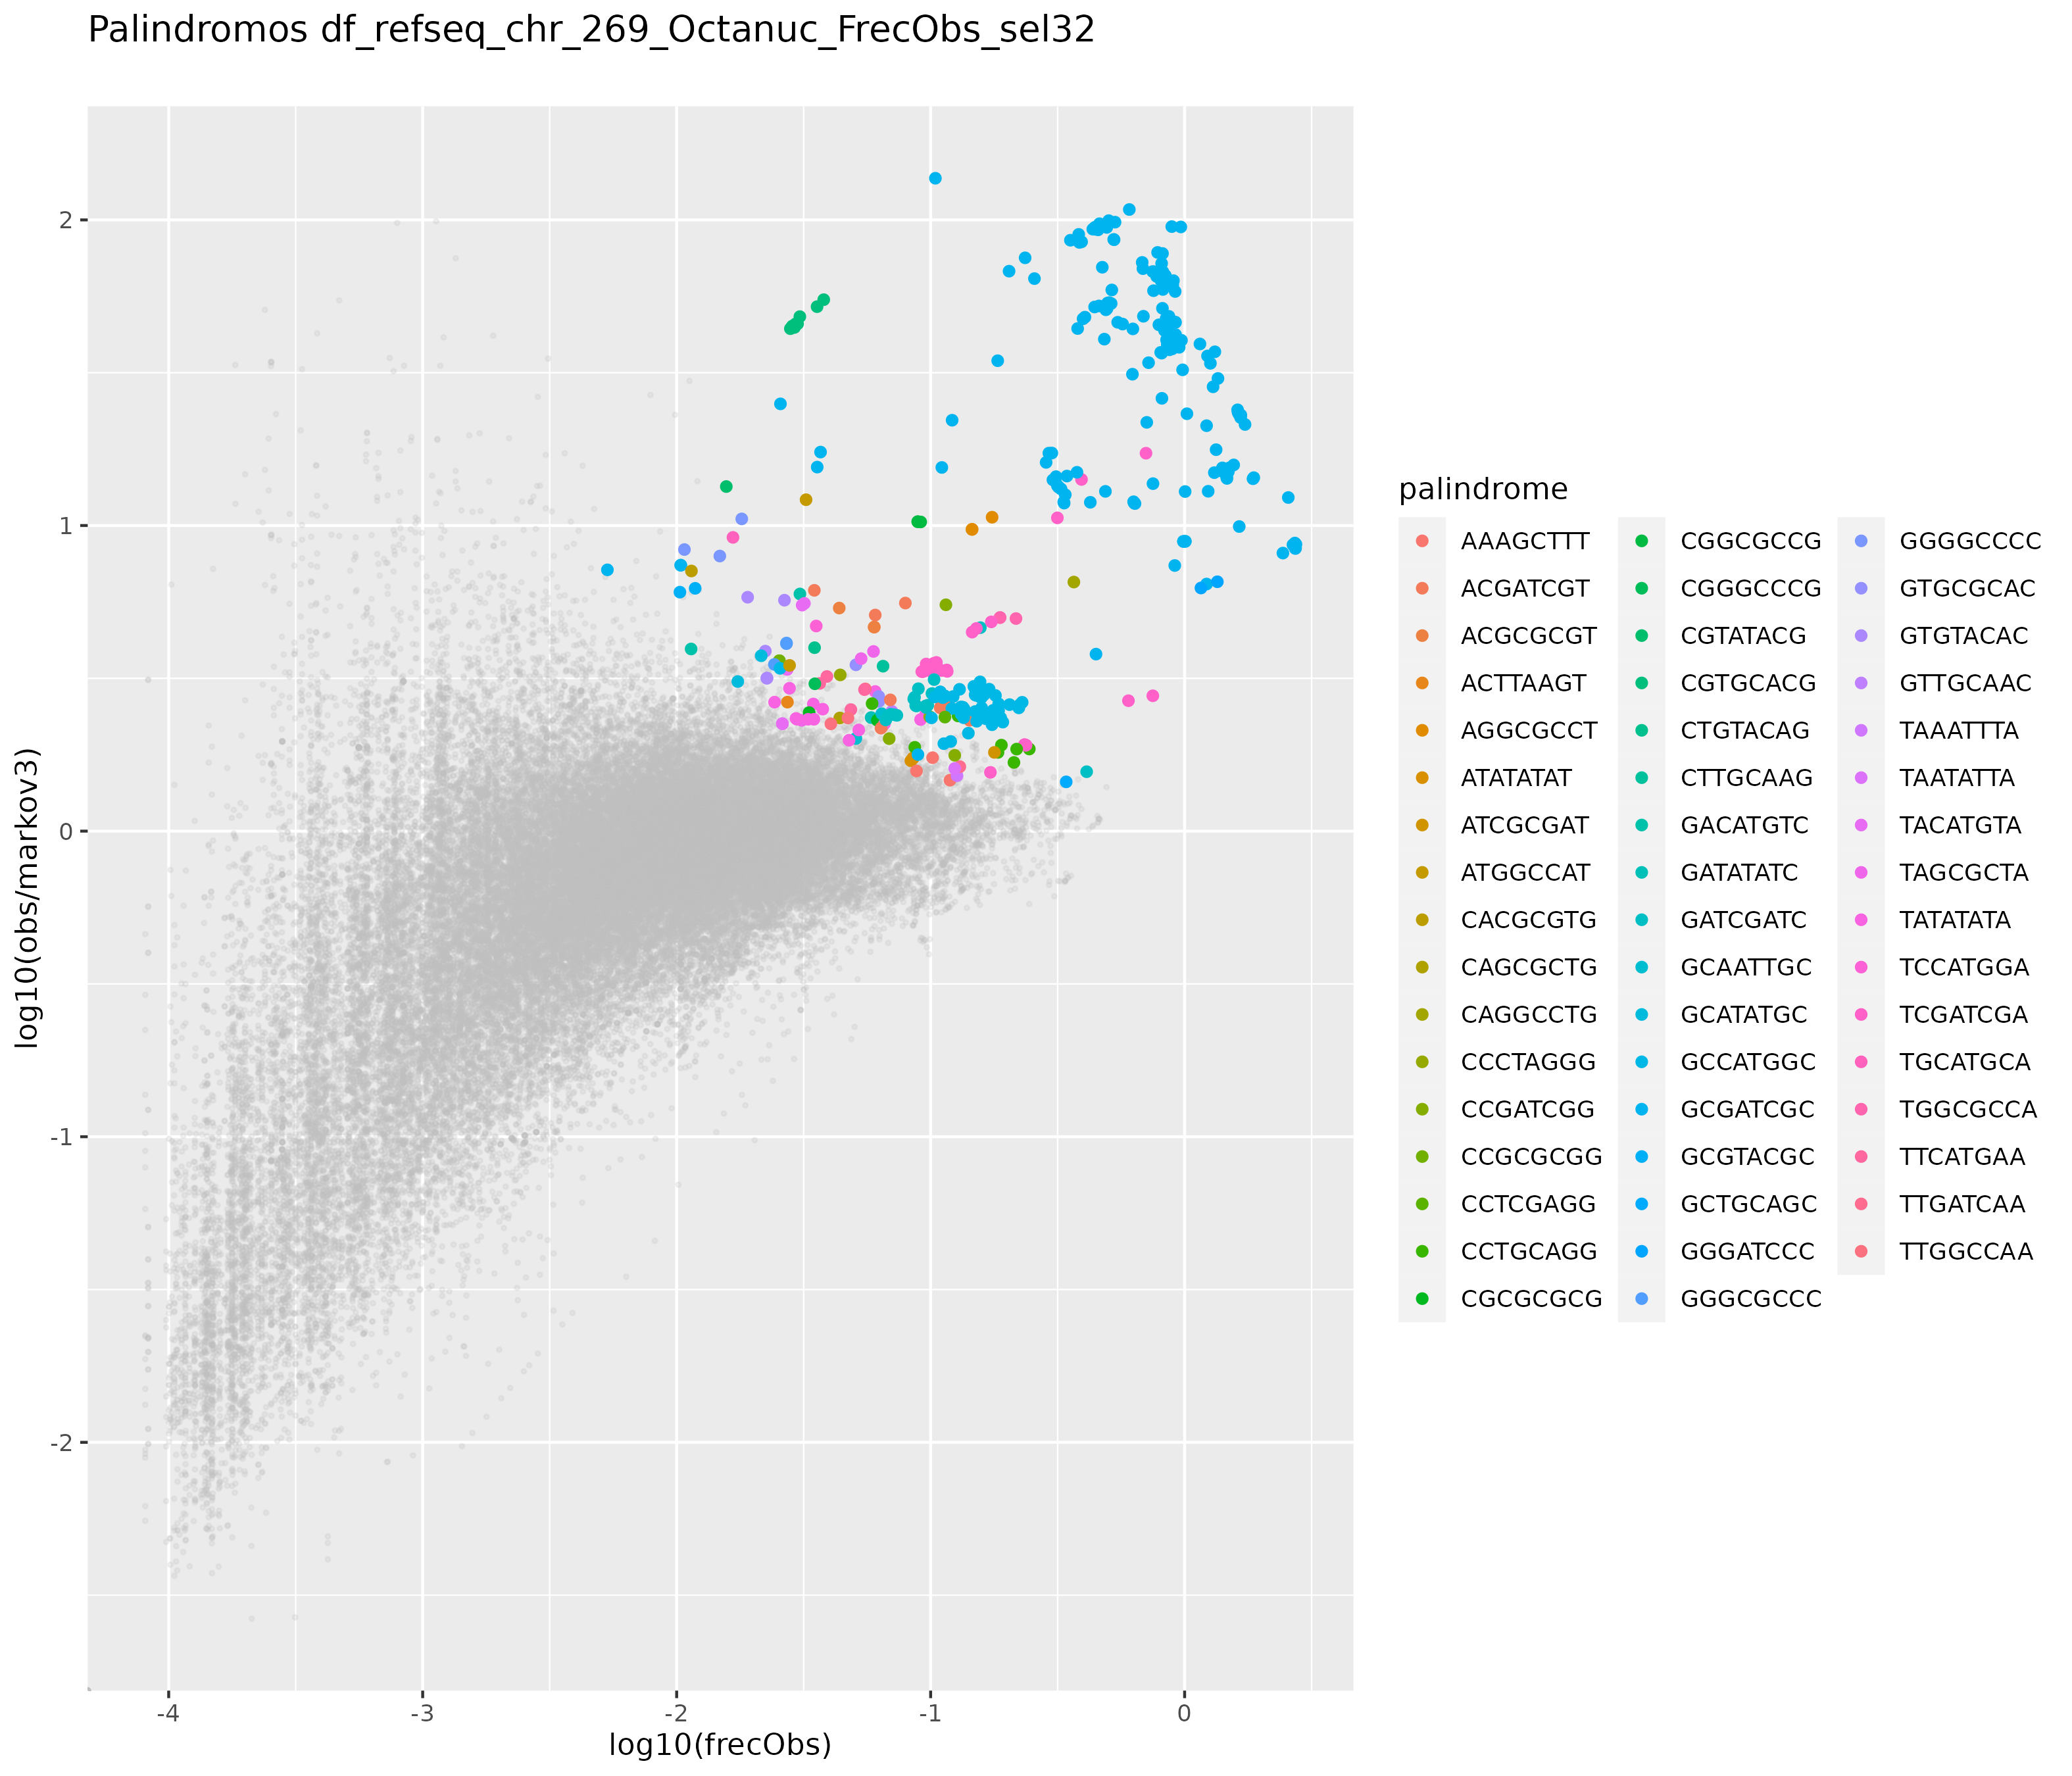
\includegraphics[width=0.8\linewidth]{figures/df_refseq_chr_269_Octanuc_FrecObs_sel32_significative-palindromes} 

}

\caption{**Enriquecimiento versus abundancia de palíndromos octámeros en el conjunto de genomas complete\_chr con un $FDR \leq 1 \times 10^{-32}$.** Enriquecimiento (**O/E**) en función de la frecuencia del motivo cada 1000 nt (**FrecObs**). Cada punto representa un palíndromo octámero de un genoma.}\label{fig:FIG1}
\end{figure}

\begin{figure}

{\centering 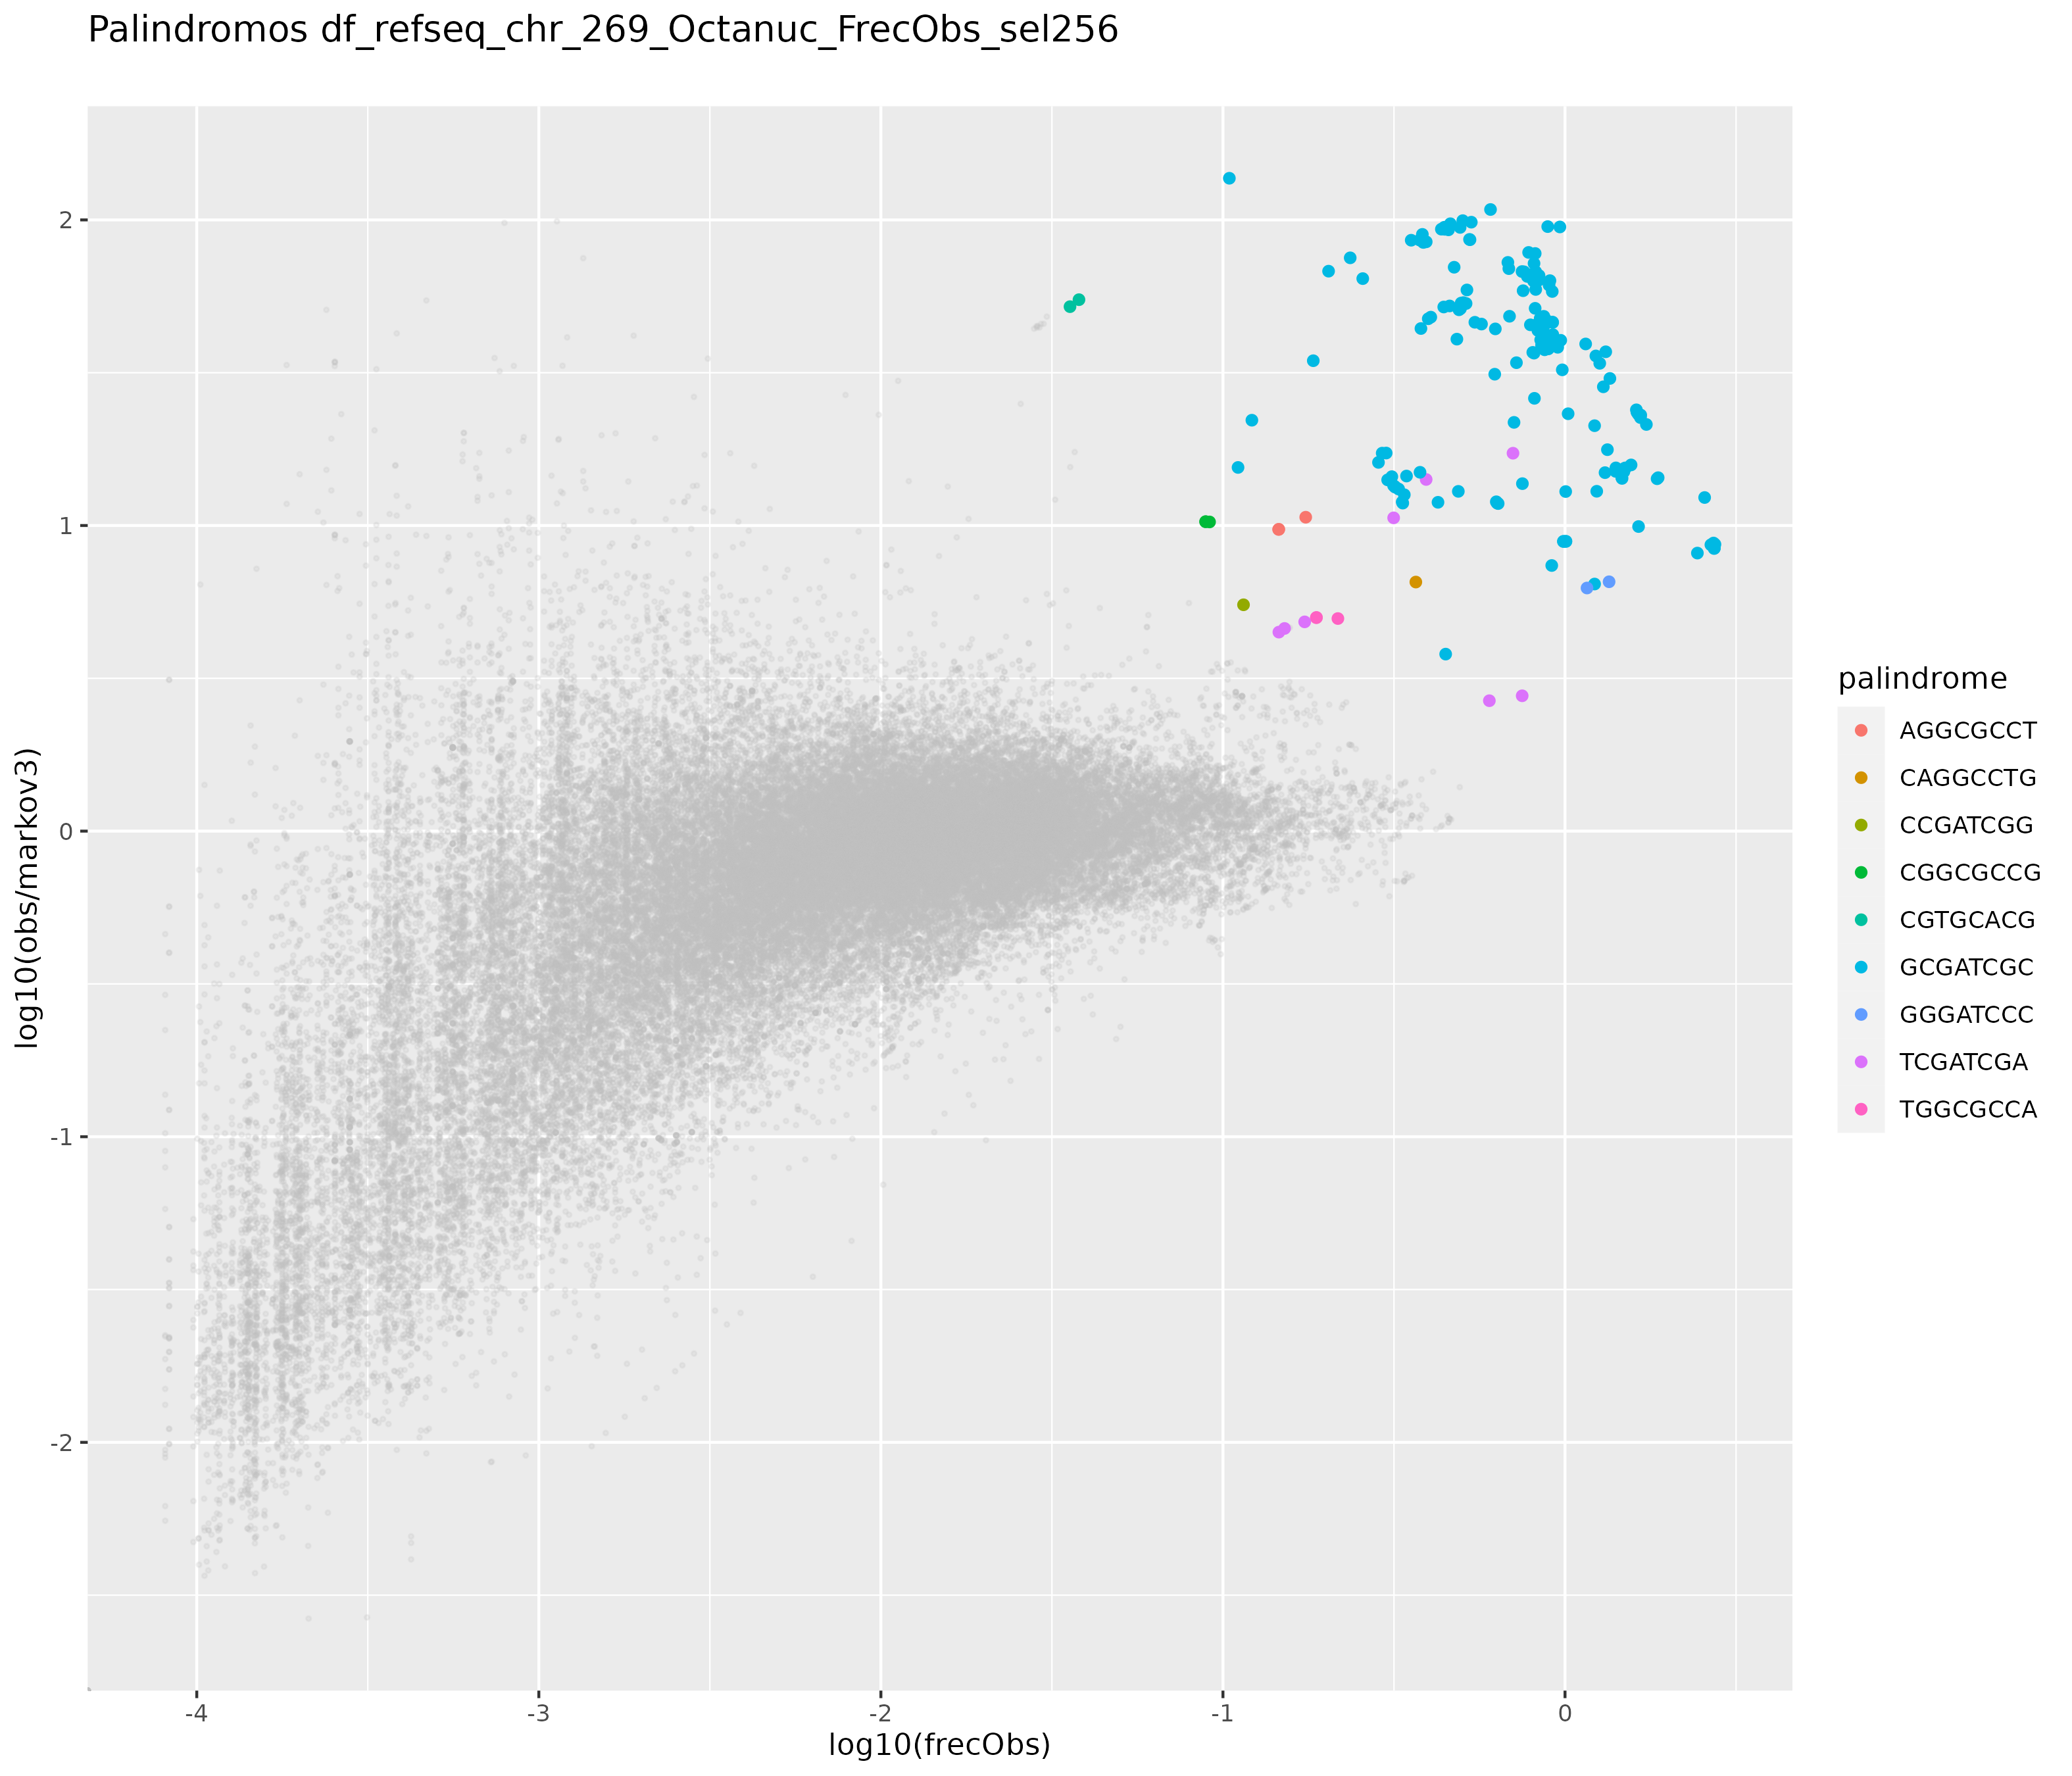
\includegraphics[width=0.8\linewidth]{figures/df_refseq_chr_269_Octanuc_FrecObs_sel256_significative-palindromes} 

}

\caption{**Enriquecimiento versus abundancia de palíndromos octámeros en el conjunto de genomas complete\_chr con un $FDR \leq 1 \times 10^{-256}$.** Enriquecimiento (**O/E**) en función de la frecuencia del motivo cada 1000 nt (**FrecObs**). Cada punto representa un palíndromo octámero de un genoma.}\label{fig:FIG2}
\end{figure}

\hypertarget{filogenia}{%
\section{Filogenia}\label{filogenia}}

Se infirieron filogenias para los dos conjuntos de genomas. Para esto usamos el software \textbf{Orthofinder} (\citet{emms2019orthofinder}), el cual utiliza \textbf{FastME} para inferir la filogenia (\citet{lefort2015fastme}). \textbf{FastME} proporciona algoritmos de distancia para inferir filogenias. FastME se basa en una evolución mínima equilibrada, que es el principio mismo de Neighbor Joining (NJ).

El software se corrió en la línea de comandos de la siguiente manera:

\begin{Shaded}
\begin{Highlighting}[]
\ExtensionTok{orthofinder}\NormalTok{ –f genomas/ }
\end{Highlighting}
\end{Shaded}

\hypertarget{anotaciuxf3n-de-la-filogenia}{%
\subsection{Anotación de la filogenia}\label{anotaciuxf3n-de-la-filogenia}}

Para tener una forma de más visual de entender la distribución de los palíndromos en los genomas, anotamos las filogenias de acuerdo a su abundancia. Se anotaron 4 filogenias según la significancia (\textbf{sel32}, \textbf{sel64}, \textbf{sel128} y \textbf{sel256}) para los 2 conjuntos de genomas. Además, esta anotación se hizo para la abundancia de acuerdo a la Frecuencia Observada por cada 1000 nucleotidos (\(FrecObs\)) (Figura \ref{fig:FIG3}) y a la tasa de Observados sobre esperados (\(OE\)) (Figura \ref{fig:FIG4}).

La anotación de las filogenias consistió en agregarles un heatmap que mostrara la abundancia de cada palíndromo y un diagrama de barras que indicara aquel palíndromo con mayor abundancia.

\begin{figure}

{\centering 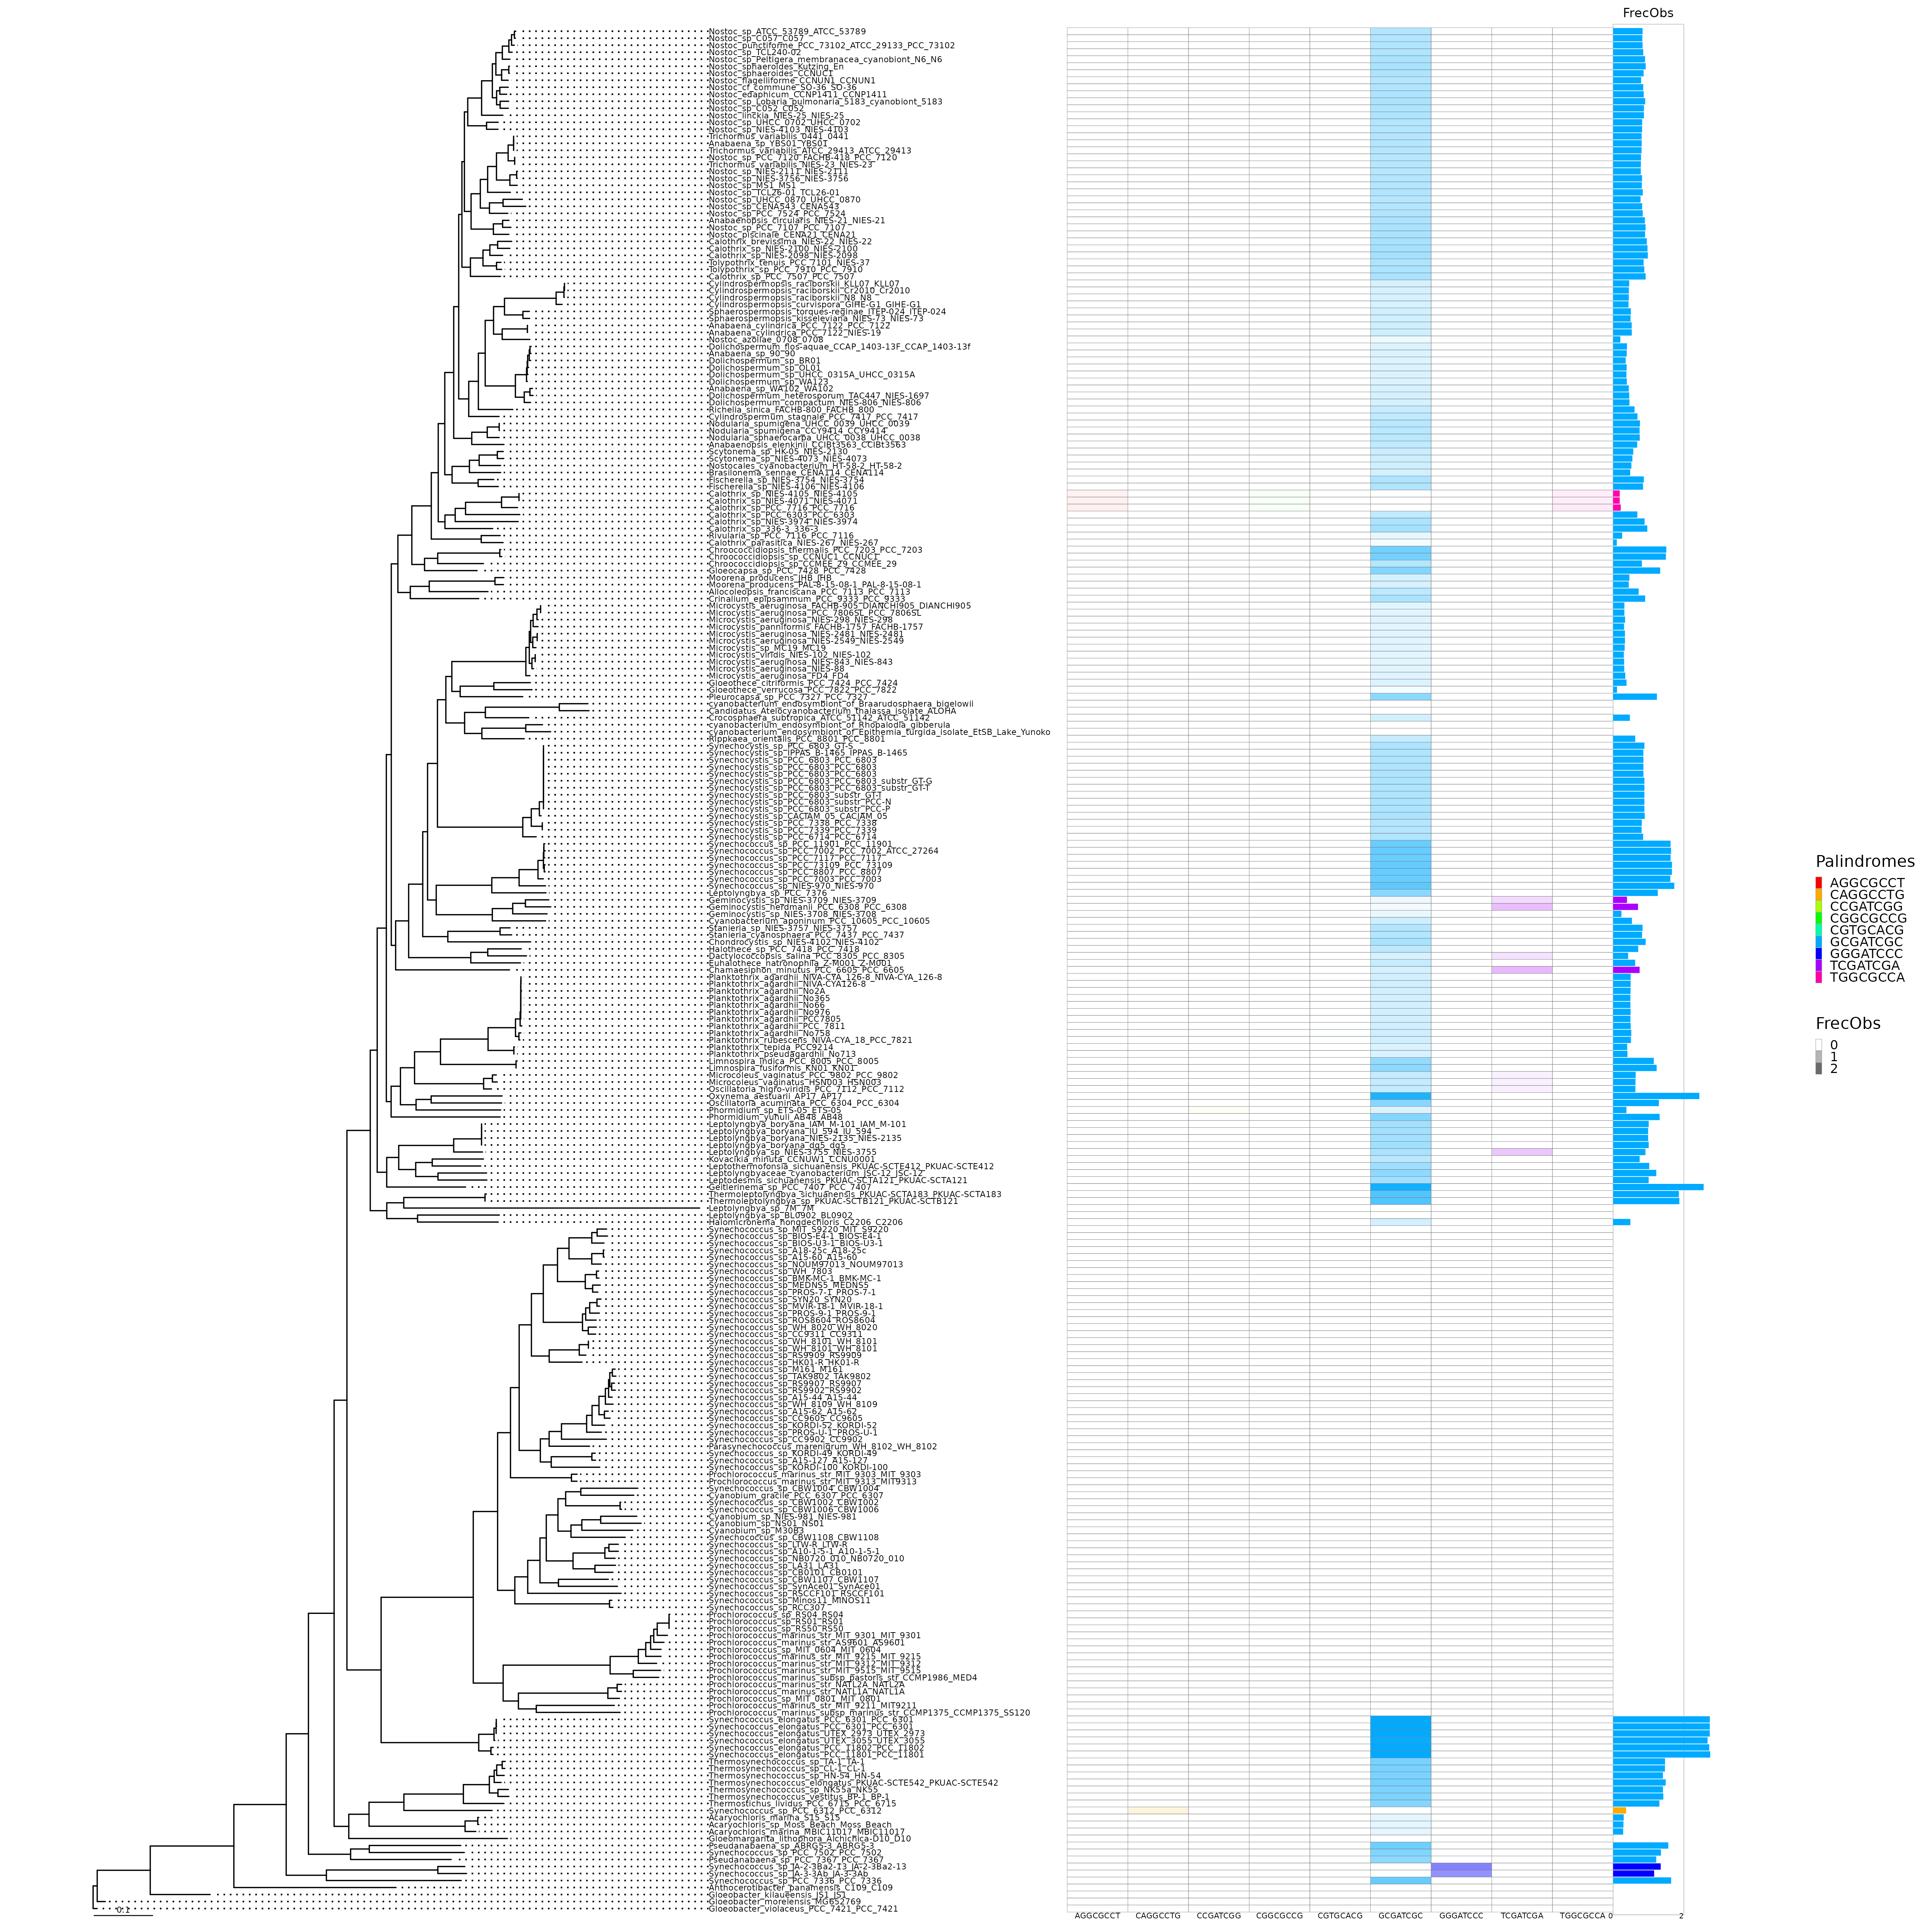
\includegraphics[width=75in]{figures/refseq_chr_269_Octanuc_FrecObs_sel256_filogenia_HIG} 

}

\caption{**Filogenia del conjunto de genomas *complete\_chr* anotada de acuerdo a la Frecuencia observada cada 1000 nt (FrecObs).** La abundancia visualizada en esta filogenia es de acuerdo al conjunto **sel256**, es decir conteos con un $FDR \leq 1 \times 10^{-256}$. La filogenia muestra 269 especies, frente a la filogenia se muestra un heatmap que indica la abundancia de cada palíndromo. Frente al Heatmap se muestra un Diagrama de barras el cual indíca el palindromo mas abundante de entre todos.}\label{fig:FIG3}
\end{figure}

\begin{figure}

{\centering 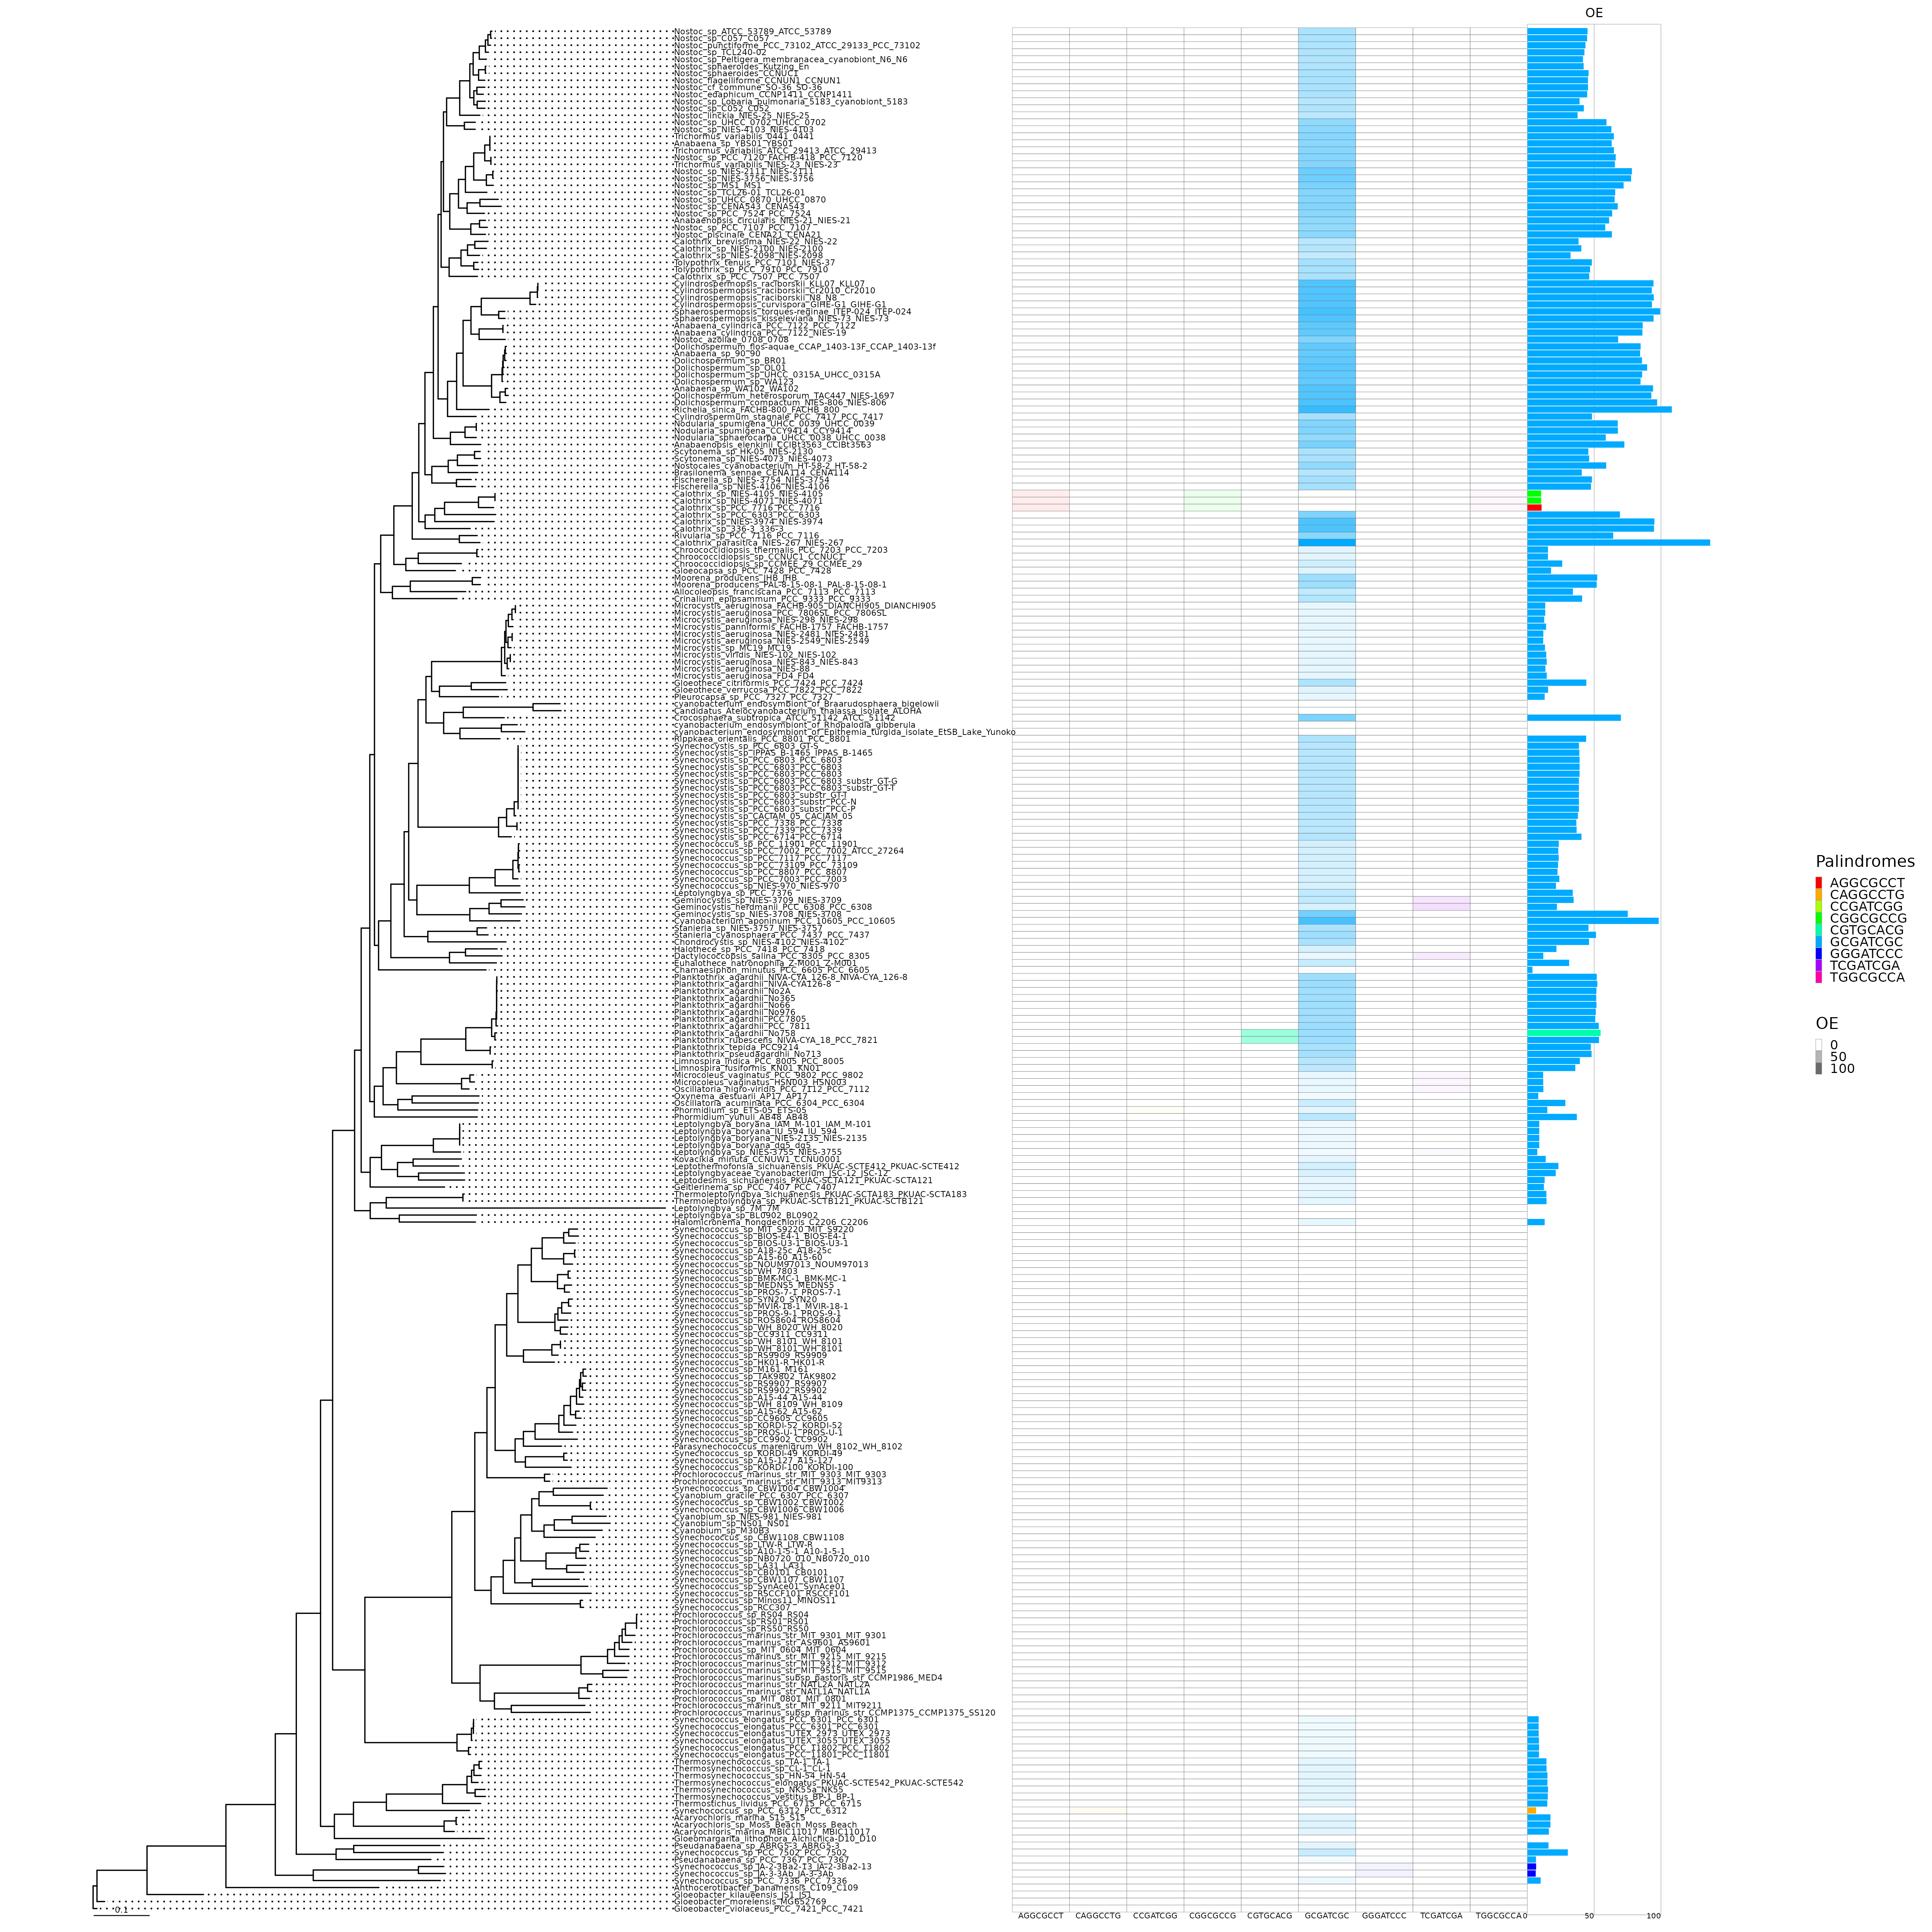
\includegraphics[width=75in]{figures/refseq_chr_269_Octanuc_OE_sel256_filogenia_HIG} 

}

\caption{**Filogenia del conjunto de genomas *complete\_chr* anotada de acuerdo a la tasa de observados sobre esperados (OE).** La abundancia visualizada en esta filogenia es de acuerdo al conjunto **sel256**, es decir conteos con un $FDR \leq 1 \times 10^{-256}$. La filogenia muestra 269 especies, frente a la filogenia se muestra un heatmap que indica la abundancia de cada palíndromo. Frente al Heatmap se muestra un Diagrama de barras el cual indíca el palindromo mas abundante de entre todos.}\label{fig:FIG4}
\end{figure}

\hypertarget{identificaciuxf3n-de-casos-relevantes}{%
\section{Identificación de casos relevantes}\label{identificaciuxf3n-de-casos-relevantes}}

De acuerdo a las filogenias anotadas, se buscaron aquellos casos en los que HIP1 o algún otro palíndromo se hubiera ganado o perdido abruptamente y en su lugar hubiese otro palíndromo abundante. Además, se buscó que en aquellos casos, las ramas en la filogenia no fueran tan largas. Esto se hizo de manera visual revisando el diagrama de barras que mostraba el palíndromo más abundante para cada especie. En total hubo 6 subclados que mostraban cambios abruptos en la abundancia de sus palíndromos (Figura \ref{fig:FIG5}).

\begin{figure}

{\centering 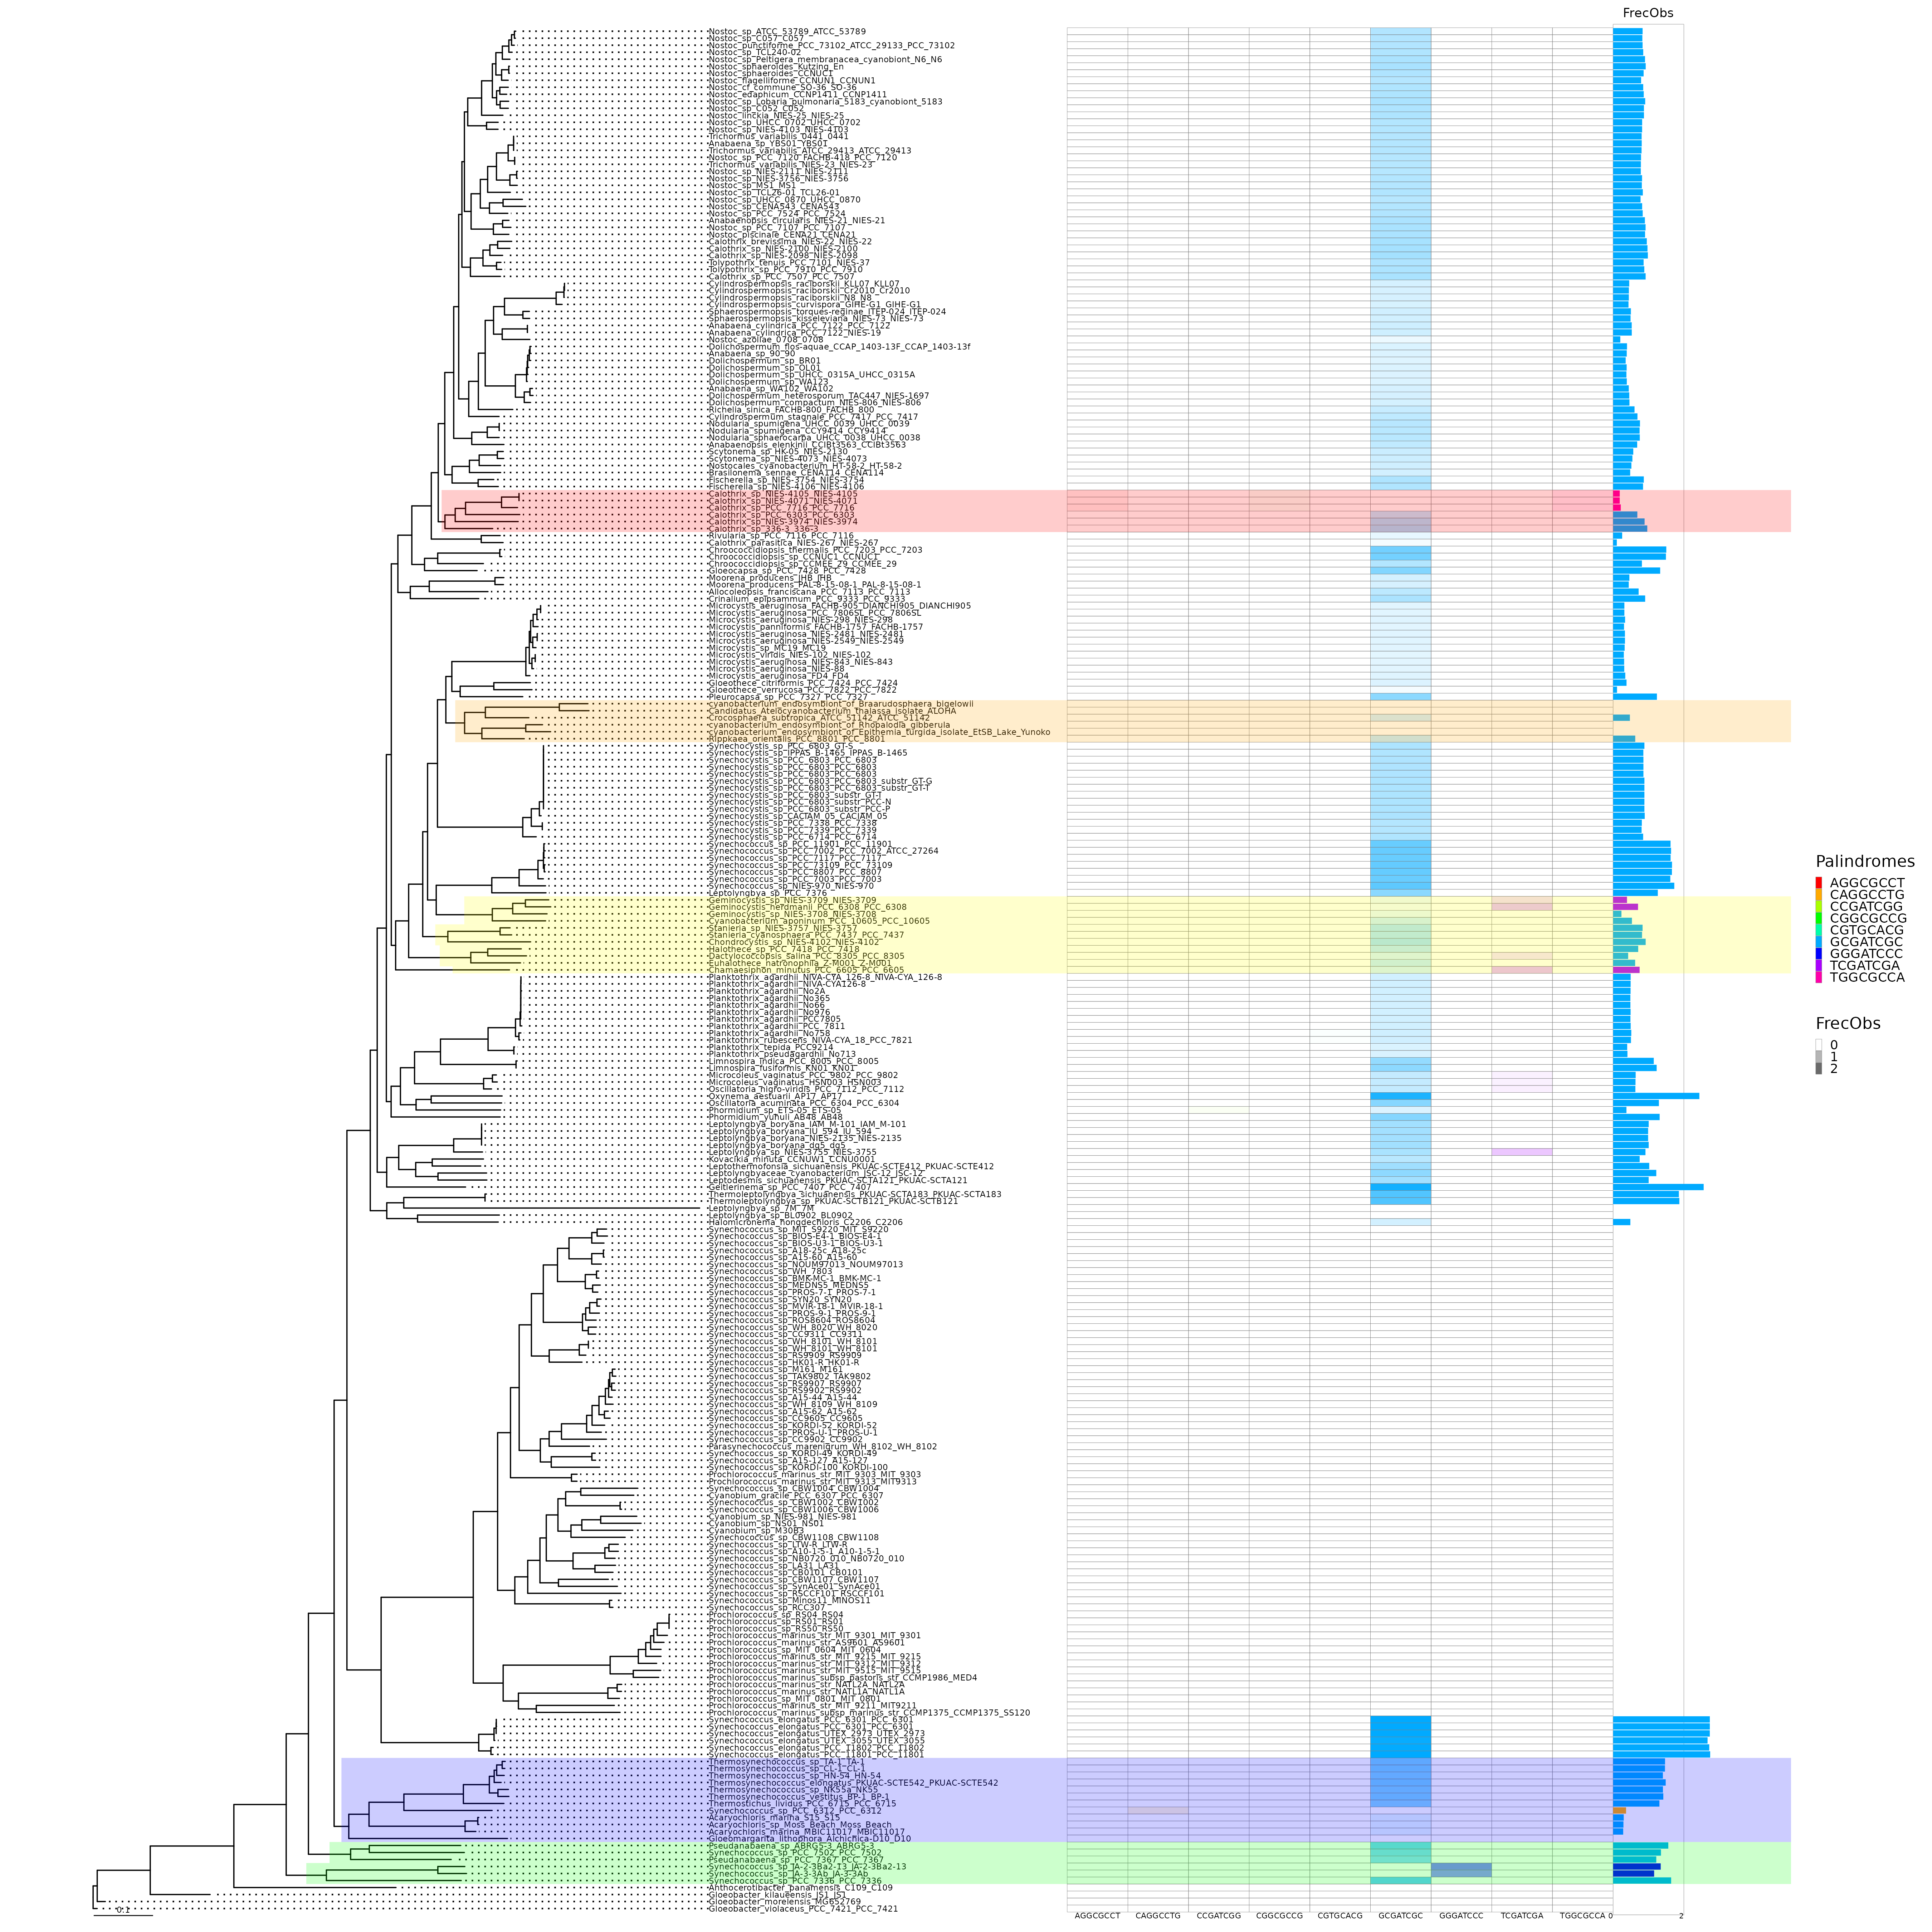
\includegraphics[width=75in]{figures/refseq_chr_269_Octanuc_FrecObs_sel256_filogenia_HIG_cases} 

}

\caption{**Casos de interés.** En la figura se muestran remarcados los casos interesantes: **clado calothrix** (rojo), **clado cyanobacterium** (naranja), **clado geminocystis** (amarillo), **clado thermosynechococcus** (azul), **clado pseudoanabaena** (verde).}\label{fig:FIG5}
\end{figure}

También se hallo un caso interesante en el conjunto \textbf{pico} (\textbf{clado A18-40}) el cual sirvió como punto de partida para analisis posteriores. En este caso se muestra que la especie Synechococcus A18-40 muestra una tasa OE mucho mayor comparada con las demás especies del clado (Figura \ref{fig:FIG6}).

\begin{figure}

{\centering 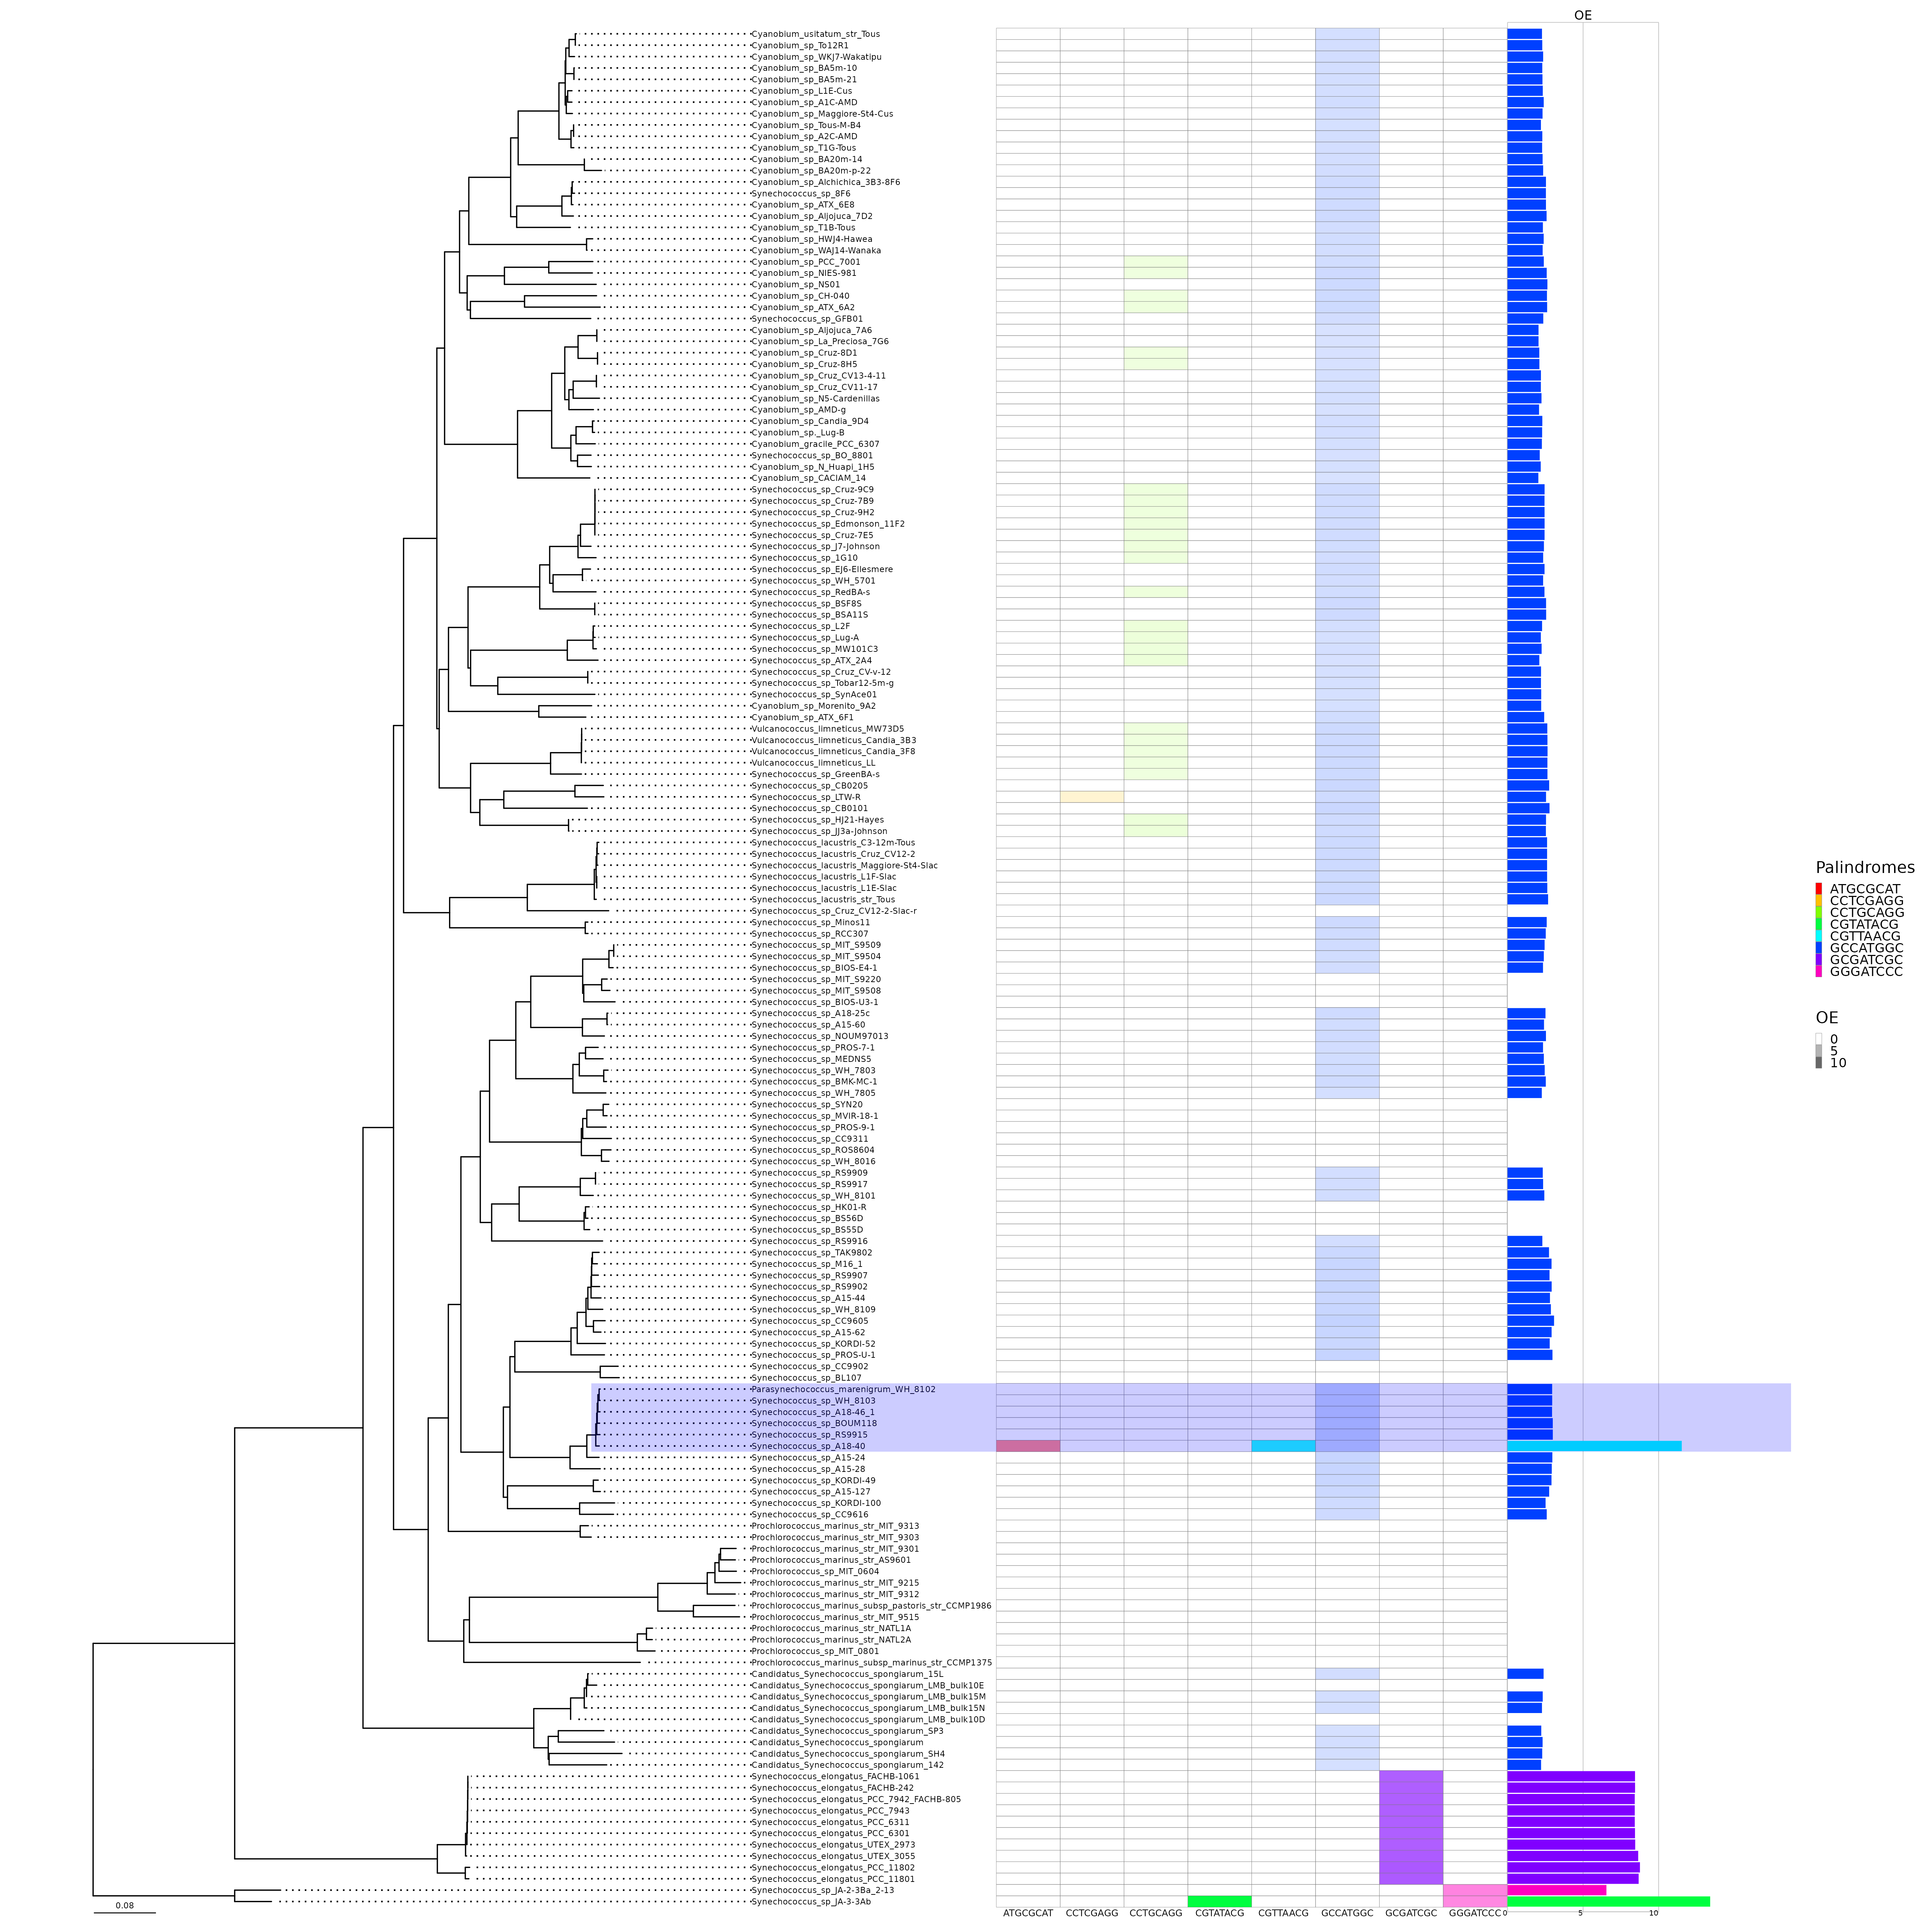
\includegraphics[width=75in]{figures/pico_165_Octanuc_OE_sel32_filogenia_HIG_cases} 

}

\caption{**Casos de interés.** En la figura se muestra remarcado el **clado A18-40** (azul).}\label{fig:FIG6}
\end{figure}

\hypertarget{reconstrucciuxf3n-ancestral-de-sitios-palindruxf3micos-en-ortuxf3logos}{%
\section{Reconstrucción Ancestral de sitios palindrómicos en ortólogos}\label{reconstrucciuxf3n-ancestral-de-sitios-palindruxf3micos-en-ortuxf3logos}}

Para tratar de entender como es que los sitios HIP1 han ido evolucionando, hicimos una reconstrucción de sitios ancestrales y posteriormente construimos varios conjuntos de redes para visualizar dicha evolución.

\hypertarget{ortuxf3logos}{%
\subsection{Ortólogos}\label{ortuxf3logos}}

Para simplificar la reconstrucción de secuencias ancestrales usamos unicamente los ortólogos. Para obtener esto usamos el pipeline \texttt{get\_homologues}:

\begin{Shaded}
\begin{Highlighting}[]
\ExtensionTok{get\_homologues.pl} \AttributeTok{{-}d}\NormalTok{ gbff }\AttributeTok{{-}t}\NormalTok{ 0 }\AttributeTok{{-}M} \AttributeTok{{-}n}\NormalTok{ PPN}
\end{Highlighting}
\end{Shaded}

Después de obtener los ortólgos filtramos:

\begin{itemize}
\tightlist
\item
  aquellos que no estuvieran en las 6 especies del clado
\item
  aquellos que tuvieran mas de una copia (parálogos)
\item
  aquellos sin sitios HIP1
\end{itemize}

\hypertarget{reconstrucciuxf3n}{%
\subsection{Reconstrucción}\label{reconstrucciuxf3n}}

Para hacer la reconstrucción usamos la pagueteria de R \texttt{phangorn}, la cual proporciona varios métodos para estimar estados de caracteres ancestrales con Máxima Parsimonia (MP) o Máxima Verosimilitud (ML). En este caso usamos ML. Adicionalmente podemos asignar los estados ancestrales según la máxima verosimilitud (``ml''):
\[P(x_r=A) = {{L(x_r=A)} \over {\sum\limits_{k\in \{A,C,G,T\}}} L(x_r= k) }\]

y el criterio de mayor probabilidad posterior (``bayes''):
\[P(x_r=A) = {{\pi_A L(x_r=A)} \over {\sum\limits_{k\in \{A,C,G,T\}}} \pi_k L(x_r= k) }\]

dónde \(L(x_r)\) es la probabilidad conjunta de los estados en las puntas y el estado en la raíz \(x_r\) y \(\pi_i\) son las frecuencias base estimadas del estado \(i\).

Toda la información de la reconstrucción fue guardada en dos tablas las cuales contienen listas de cada transicion entre cada estado. Estas tablas fueron creadas con la siguiente función:

\begin{Shaded}
\begin{Highlighting}[]
\FunctionTok{source}\NormalTok{(}\StringTok{"ASR\_Orth\_Functions/NodeAndEdges.R"}\NormalTok{)}

\FunctionTok{Create\_Transition\_Table}\NormalTok{ (}\AttributeTok{SitesTable =} \StringTok{"Clados/Callothrix\_clade/PALINDROMES/GCGATCGC/Orthologues\_Palindrome\_sites.txt"}\NormalTok{,}
                                \AttributeTok{EvolutionModel =} \StringTok{"F81"}\NormalTok{,}
                                \AttributeTok{Method =} \StringTok{"bayes"}\NormalTok{,}
                                \AttributeTok{Phylogeny =} \StringTok{"Clados/Callothrix\_clade/SpeciesTree\_rooted.txt"}\NormalTok{,}
                                \AttributeTok{OrthoPath =} \StringTok{"Clados/Callothrix\_clade/PALINDROMES/GCGATCGC/Only\_ORTHOLOGUES/"}\NormalTok{)}
\end{Highlighting}
\end{Shaded}

\hypertarget{resultados}{%
\chapter{RESULTADOS}\label{resultados}}

Acontinucación se presentan los resultados en cuatro secciones:

\begin{itemize}
\item
  La \textbf{Seccion I} muestra los analisis de la distribución de los sitios palindromicos a través de los ortólogos y marcos de lectura de las especies.
\item
  La \textbf{Sección II} muestra una serie de resultados de la reconstrucción ancestral de los sitios palindrómicos HIP1 y TGGCGCCA unicamente para el clado Calothrix.
\item
  La \textbf{Sección III} muestra una serie de resultados de la reconstrucción ancestral de los sitios palindrómicos HIP1 y TGGCGCCA unicamente para el clado Thermosynechococcus.
\item
  La \textbf{Sección IV} muestra los resultados del análisis de sitios CGTTAACG en el clado A18-40.
\item
  La \textbf{Sección V} muestra los resultados del análisis de sitios repetidos en el los clados.
\item
  La \textbf{Sección VI} muestra una serie de resultados de la reconstrucción ancestral de los sitios palindrómicos HIP1 para los clados Cyanobacterium, Geminocystis y Pseudoanabaena.
\end{itemize}

\hypertarget{secciuxf3n-i}{%
\chapter*{Sección I}\label{secciuxf3n-i}}
\addcontentsline{toc}{chapter}{Sección I}

\hypertarget{distribuciuxf3n-de-hip1-en-los-marcos-de-lectura}{%
\section{Distribución de HIP1 en los marcos de lectura}\label{distribuciuxf3n-de-hip1-en-los-marcos-de-lectura}}

Para el analisis de los sitios palindrómicos primero se hizo un conteo de lo sitios en cada especie de cada clado para luego tomar aquella especie que tuviera la mayor cantidad de sitios posibles. Esto con el fin de tener mas sitios para analizar. Aquellas especies con la mayor cantidad de sitios se muestran resaltadas en amarillo en la Tabla \ref{tab:HighestSites}.

Para ver como es la distribución de los sitios HIP1 a traves del genoma hicimos un conteo de sitios en cada marco de lectura (Tabla \ref{tab:TABMuts2}).

\hypertarget{reconstrucciuxf3n-de-sitios-ancestrales-en-ortuxf3logos-del-clado-calothrix.}{%
\chapter{Reconstrucción de sitios ancestrales en ortólogos del clado Calothrix.}\label{reconstrucciuxf3n-de-sitios-ancestrales-en-ortuxf3logos-del-clado-calothrix.}}

\hypertarget{filogenia-1}{%
\section{Filogenia}\label{filogenia-1}}

Este análisis se centra en el subclado Calothrix el cual está compuesto de 6 especies. La importancia de este clado radica en que 3 de las especies (\textbf{Calothrix sp. 336/3}, \textbf{Calothrix sp. NIES 3974} y \textbf{Calothrix sp. PCC 6303}) de este clado contienen alta abundancia de sitios \textbf{GCGATCGC} mientras que las otras 3 especies (\textbf{Calothrix PCC 7716}, \textbf{Calothrix sp. NIES 4071} y \textbf{Calothrix sp. NIES 4105}) tienen muy baja o nula abundancia de sitios. Sin mencionar que, estas últimas tres especies muestran una abundancia significante de otro palíndromo, el cual se encuentra en muy baja (o nula) abundancia en las otras tres especies (Figura \ref{fig:FIG1}). Entendido esto, se creó una filogenia con las 6 especies y una adicional (\textbf{Calothrix parasitica NIES 267}) como grupo externo. Esto último para evitar un sesgo en los resultados (Figura \ref{fig:FIG2}).

\begin{figure}

{\centering 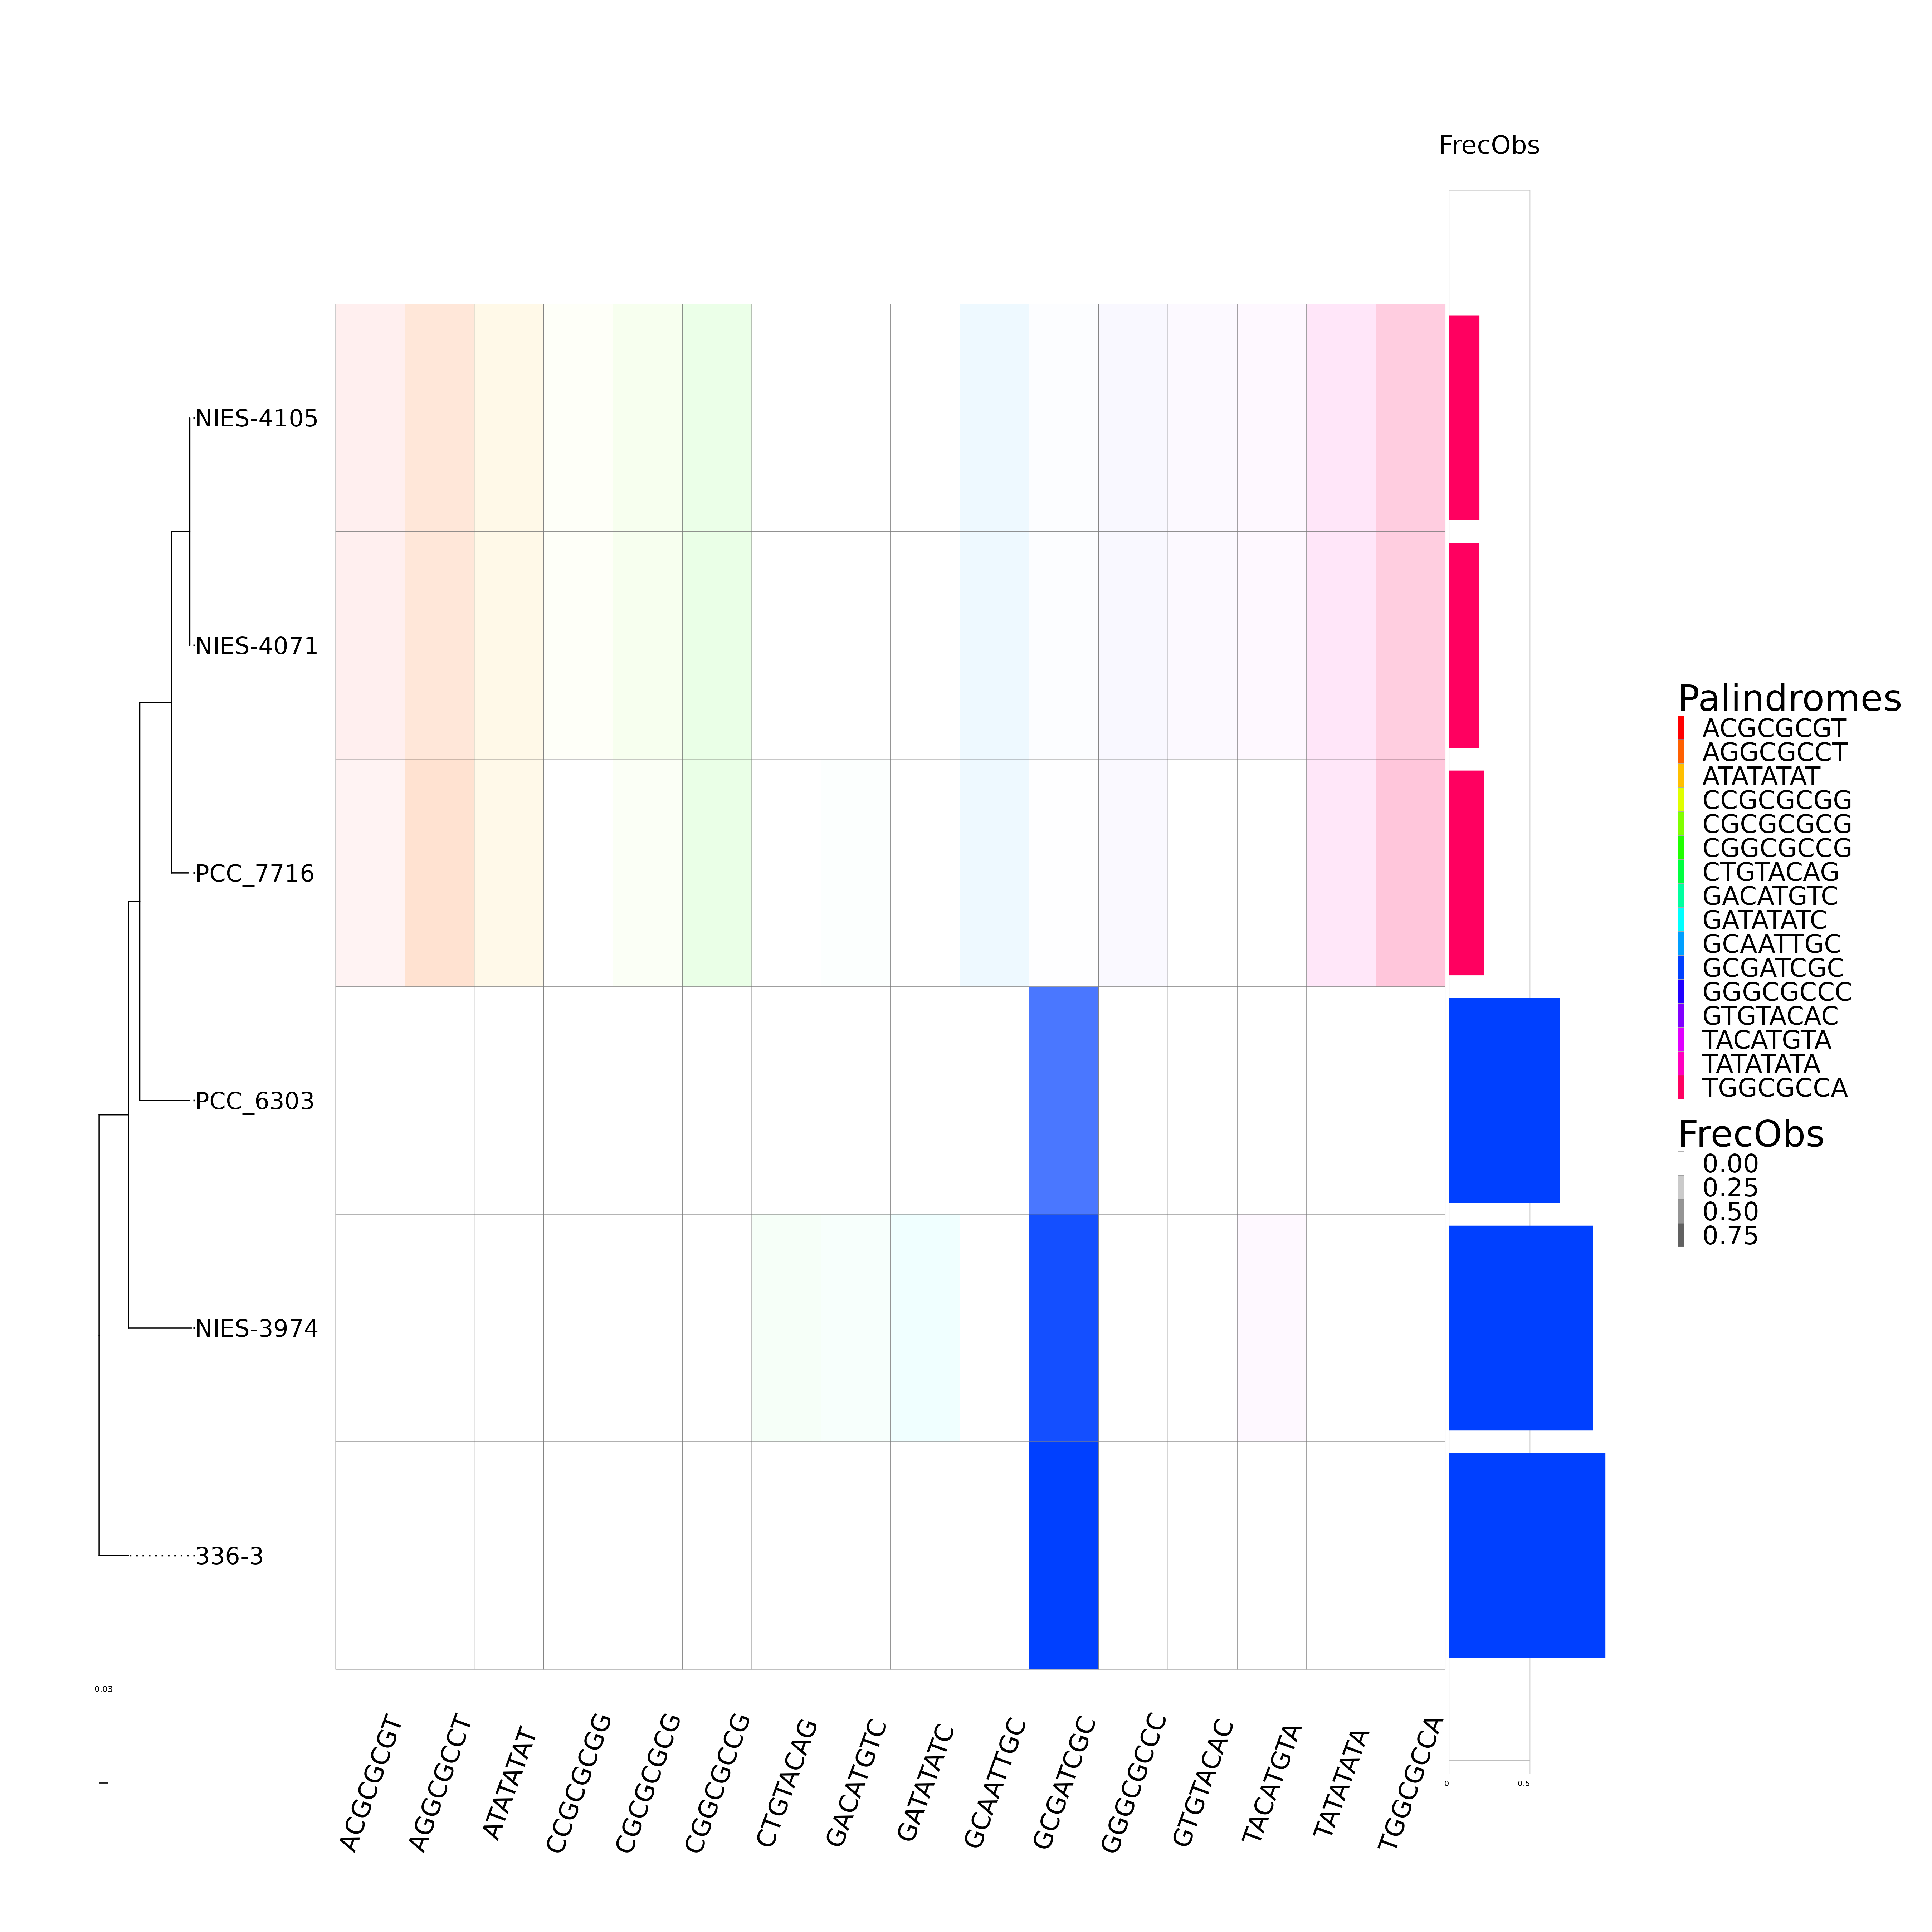
\includegraphics[width=0.8\linewidth]{Clados/Callothrix_clade/figures/Calothrix_Octanuc_FrecObs_sel32_filogenia_HIG} 

}

\caption{**Filogenia anotada del clado Calothrix.** En esta figura podemos ver la filogenia del clado calothrix, un heatmap que indica la frecuencia Observada por cada 1000 nts de cada octámero palindrómico en cada una de las especies y un barplot que muestra aquel octamero mas abundante.}\label{fig:FIG1}
\end{figure}

\begin{figure}

{\centering 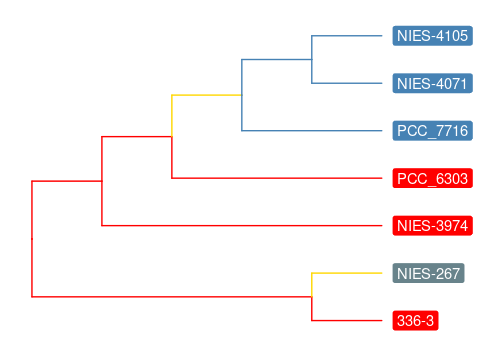
\includegraphics[width=0.8\linewidth]{ENG_files/figure-latex/FIG2-1} 

}

\caption{**Filogenia del clado Calothrix.** En esta figura podemos ver la filogenia del clado calothrix. En azul vemos el subclado que contiene abundancia de sitios GCGATCGC y en rojo el subclado con abundancia de sitios TGGCGCCA. En amarillo se muestra la transición del nodo 9 al 10 la cual es de interes ya que es el momento en la que las abundancias de los palíndromos cambian. En gris se muestra a la especie **Calothrix parasitica NIES 267** como grupo externo.}\label{fig:FIG2}
\end{figure}

\hypertarget{ortuxf3logos-1}{%
\section{Ortólogos}\label{ortuxf3logos-1}}

Los sitios para este análisis se obtuvieron de los ortólogos entre las 7 especies (subclado + el grupo externo). Posteriormente se filtraron todos aquellos ortólogos que no eran de utilidad. Es decir, ortólogos sin sitios y parálogos. Finalmente, dependiendo la especie a revisar, estos ortólogos se filtraban para realizar una alineación múltiple y buscar los sitios palindrómicos.

\hypertarget{buxfasqueda-de-sitios-gcgatcgc}{%
\section{Búsqueda de sitios GCGATCGC}\label{buxfasqueda-de-sitios-gcgatcgc}}

Para hacer esto primero filtramos todos los ortólogos que tuvieran al menos sitio \textbf{GCGATCGC} en una de las 3 especies con alta abundancia (\textbf{Calothrix sp. 336/3}, \textbf{Calothrix sp. NIES 3974} o \textbf{Calothrix sp. PCC 6303} remarcadas en el subclado azul de la filogenia) (Figura \ref{fig:FIG2}). En un inicio esto se hizo para partir del conjunto con el mayor número de sitios posibles y así poder tener una mayor cantidad de datos. Sin embargo, después de revisar la distribución de los sitios en todas las especies. Se decidió, hacer un análisis para cada una de las especies como referencia. Además, los sitios hallados también se clasificaron de acuerdo al marco de lectura en el que estaban situados. Por lo tanto, se crearon 4 conjuntos dependiendo la especie en donde se buscaron y 3 subconjuntos para cada marco de lectura.

El primer conjunto corresponde a los sitios hallados en la especie \textbf{Calothrix sp. 336/3} (\textbf{336-3}) el cual contiene \textbf{2407} sitios y corresponde al \textbf{58\%} de los sitios totales entre las tres especies antes mencionadas (Figura \ref{fig:FIG3}A). El segundo conjunto corresponde a los sitios hallados cuando se usó a \textbf{Calothrix sp. NIES 3974} (\textbf{NIES-3974}) como referencia, contiene \textbf{2370} sitios y corresponde al \textbf{57\%} de los sitios (Figura \ref{fig:FIG3}B). El tercer conjunto tiene a \textbf{Calothrix sp. PCC 6303} (\textbf{PCC\_6303}) como referencia y contiene \textbf{1887} sitios que corresponden al \textbf{46\%} de los sitios totales (Figura \ref{fig:FIG3}C). Finalmente se usó un conjunto de sitios únicos entre las tres especies el cual contiene \textbf{2447} sitios que corresponden al \textbf{59\%} de los sitios totales (Figura \ref{fig:FIG3}D).

\begin{figure}

{\centering 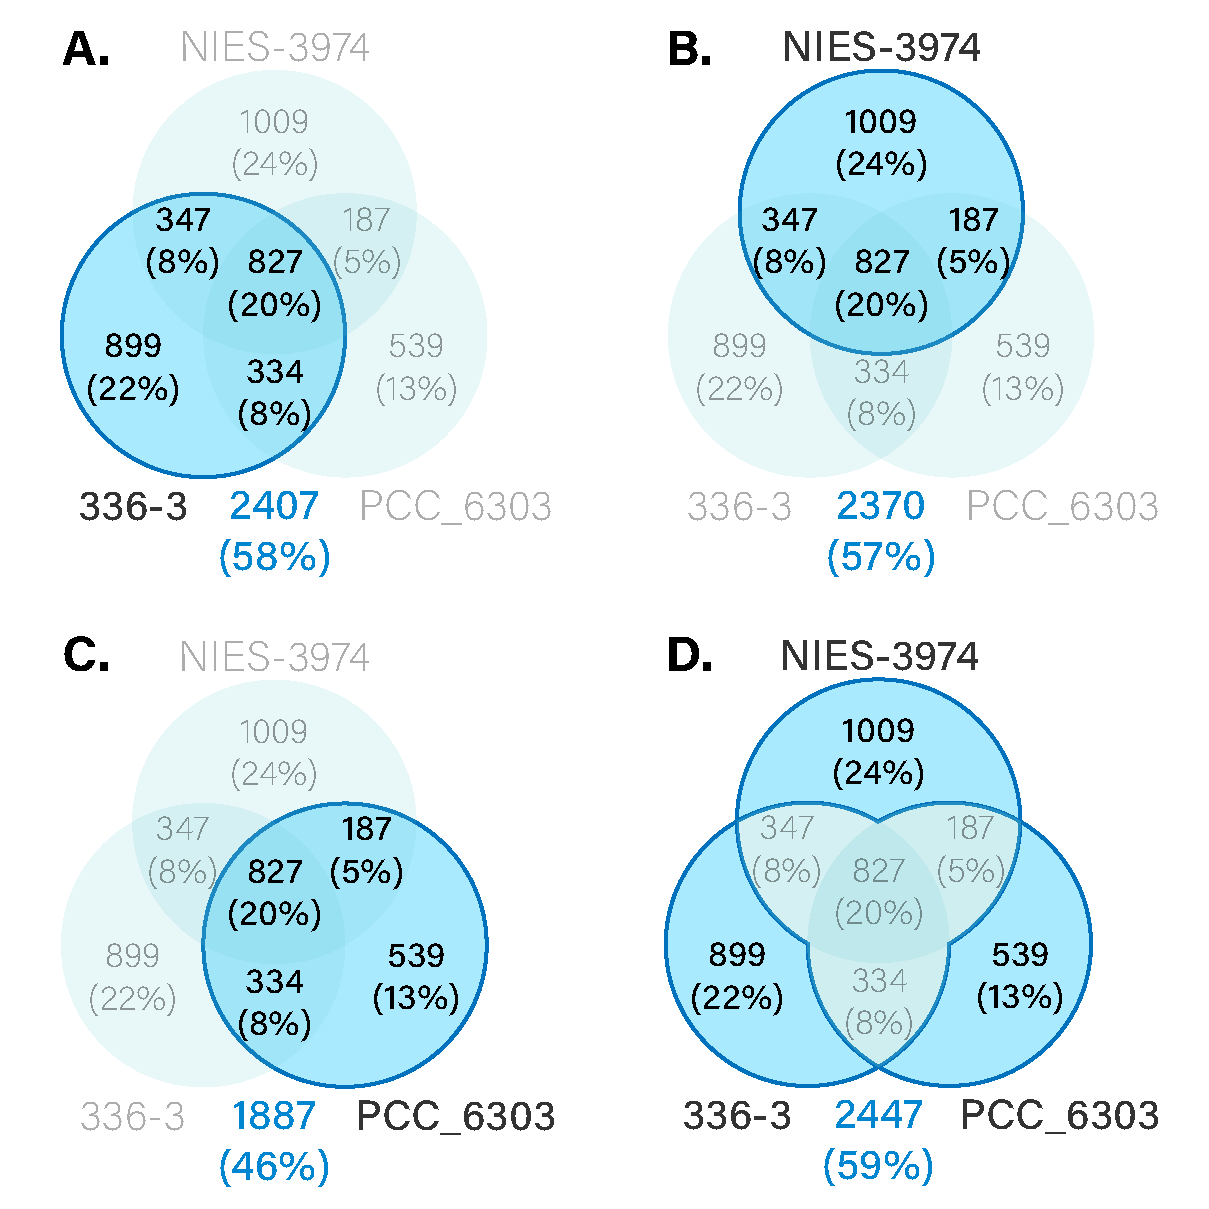
\includegraphics[width=0.8\linewidth]{Clados/Calothrix_B/figures/All_venn_calothrix} 

}

\caption{**Conjuntos de sitios.** En esta figura podemos ver los 4 conjuntos de sitios de acuerdo a la especie de referencia. El texto en azul se muestra la cantidad de sitios del conjunto y el porcentaje de los sitios totales que representa.}\label{fig:FIG3}
\end{figure}

Una vez obtenidos los conjuntos de sitios, se hizo una reconstrucción ancestral para cada conjunto, se cuantificaron todas las sustituciones para cada transición entre cada nodo de la filogenia y se clasificaron de acuerdo a como cambiaba el aminoácido de un nodo al siguiente.

\hypertarget{transiciones-entre-los-nodos}{%
\section{Transiciones entre los nodos}\label{transiciones-entre-los-nodos}}

Es importante resaltar que debido a que los sitios \textbf{GCGATCGC} contienen únicamente 8 nucleótidos, se agregaron nucleótidos rio abajo o arriba del sitio, esto dependiendo el marco de lectura. Para el marco de lectura 1 se agregó un nucleótido al final para completar el 3er codón. Para el marco de lectura 2 se agregó un nucleótido al inicio para completar el primer codón. Finalmente, para el marco de lectura 3 se agregaron 2 nucleótidos al inicio y dos al final de la secuencia para completar el 1er y el 4to codón. Esto se hizo para poder tener una secuencia de AA que abarcara todo el sitio. Sin embargo, agregar estos nucleótidos planteó el agregar un tipo de transiciones particulares en las que, si bien el aminoácido cambia de un nodo a otro, dicho cambio se da sin alterar el sitio palindrómico en sí. Esto es porque la mutación puede caer en los nucleótidos que se agregaron para completar los codones y no en el sitio en sí.

Por lo tanto, los cambios entre un nodo y el siguiente pueden ser de 7 tipos y se explican a continuación.

\begin{itemize}
\item
  \textbf{Conservative.} La secuencia de AA cambió en la transición, pero tiene similitud de acuerdo al score de BLOSUM62.
\item
  \textbf{ConservativeNoSiteMut.} La secuencia de AA cambió en la transición, pero tiene similitud de acuerdo al score de BLOSUM62. Sin embargo, a pesar de este cambio, el sitio GCGATCGC no sufrió mutaciones.
\item
  \textbf{Deletion.} La secuencia de AA tuvo una o más deleciones en la transición.
\item
  \textbf{NoMutation.} La secuencia de AA no sufrió mutaciones. Es decir, la secuencia pasó sin cambios al siguiente nodo.
\item
  \textbf{NoSynonym.} La secuencia de AA cambió en la transición
\item
  \textbf{NoSynonymNoSiteMut.} La secuencia de AA cambió en la transición. Sin embargo, el sitio GCGATCGC no sufrió mutaciones.)
\item
  \textbf{Synonym.} El sitio sufrió mutaciones. Sin embargo, la secuencia de AA no cambió en la transición.
\end{itemize}

\hypertarget{filogenias-anotadas}{%
\section{Filogenias anotadas}\label{filogenias-anotadas}}

Una vez cuantificadas todas las mutaciones de las transiciones se anotó una filogenia para visualizar la frecuencia del tipo de cambios que se daban en cada nodo. Esta anotación se hizo para cada conjunto de sitios y cada marco de lectura. Cada conjunto se muestra en una sola figura la cual contiene 3 filogenia con diagramas de pie en cada nodo. Dicho diagrama corresponde a las proporciones de todos los tipos de cambio que se dieron en la transición desde el nodo anterior al siguiente (Figura \ref{fig:EXA}). Por lo tanto, las proporciones que se muestran en los diagramas de cada nodo corresponden a lo que sucedió con la secuencia de AA desde el nodo parental hacia el nodo en el que se encuentra el diagrama. La filogenia también muestra un diagrama de venn que muestra el conjunto de sitios usado (de acuerdo a la especie de referencia).

\hypertarget{condiciones-de-interuxe9s}{%
\section{Condiciones de interés}\label{condiciones-de-interuxe9s}}

Dado que una de las preguntas esenciales sobre los sitios \textbf{GCGATCGC} es como es que se pierden (o ganan), separamos los resultados en 3 conjuntos los cuales debían cumplir ciertas condiciones de interés.

El primer conjunto de resultados (\textbf{Ancestor}) muestra solo aquellos sitios en los que en la transición partió de un sitio \textbf{GCGATCGC}. En dicha transición el sitio pudo haberse conservado, cambiado o eliminado en el siguiente nodo.

El segundo conjunto (\textbf{Actual}) muestra solo aquellos sitios en los que la transición condujo a un sitio \textbf{GCGATCGC} a partir de un sitio que no lo era anteriormente. Es decir, aquellas transiciones que partieron de \textbf{GCGATCGC} y concluyeron en \textbf{GCGATCGC} (no tuvieron cambios) no se cuentan en este conjunto

El tercer conjunto (\textbf{All}) muestra todas las transiciones que se dieron en todos los sitios de la especie de referencia. Este conjunto muestra lo que pasa en cada transición entre cada nodo sin importar si se parte de un sitio \textbf{GCGATCGC} o si se llega al mismo.

Un ejemplo de lo que pasa en las figuras se muestra en las figuras \ref{fig:FIG4} y \ref{fig:EXA}.

\begin{figure}

{\centering 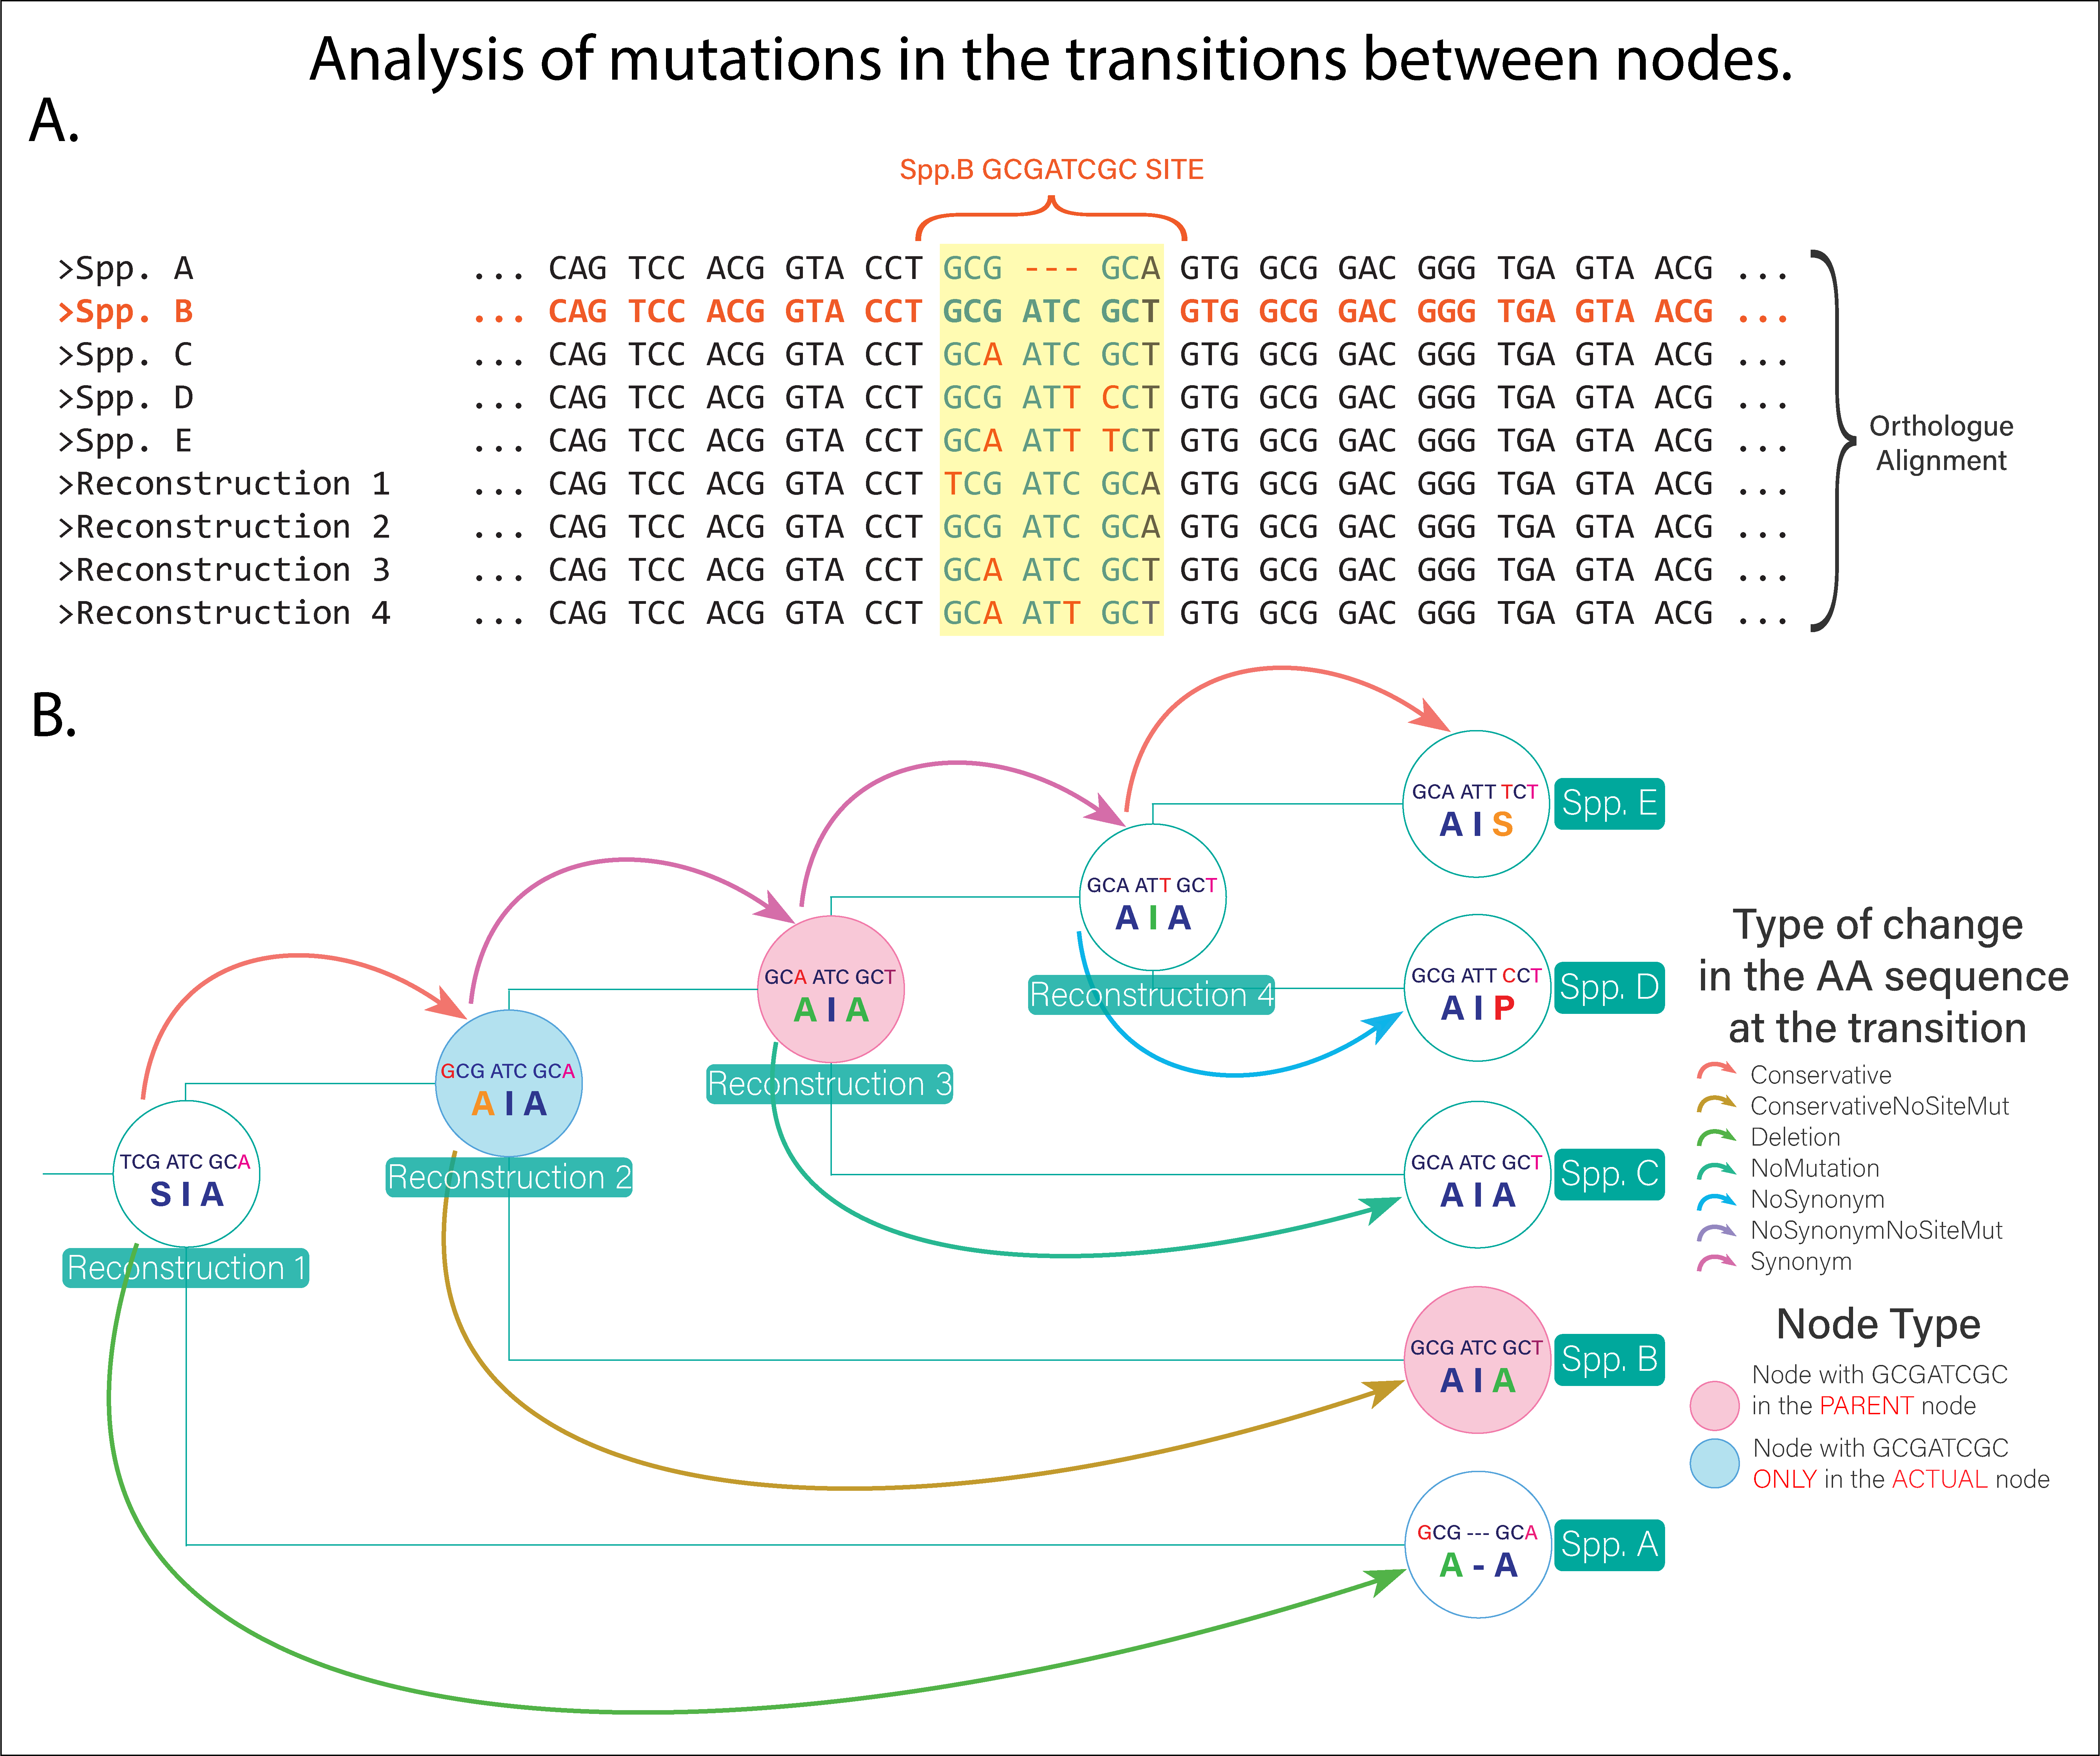
\includegraphics[width=1\linewidth]{Clados/Calothrix_B/figures/Reconstruction_explanation} 

}

\caption{**Ejemplo de como se leen los diagramas de pie.** En esta figura podemos observar como es que se contruyen los diagramas de pie a lo largo de los nodos. Cada diagrama representa las proporciones de tipos de cambio que sufrieron aminoacidos en cada transición.}\label{fig:FIG4}
\end{figure}

\begin{figure}

{\centering \includegraphics[width=1\linewidth]{Clados/Calothrix_B/figures/transition example} 

}

\caption{**Proceso para anotar las filogenias de acuerdo a las transiciones.** En la Figura A se muestra (remarcado en un cuadro amarillo) el sitio GCGATCGC alineado a lo largo de las especies y las recosntrucciones. En la Figura B se muestra la reconstrucción acomodada en la filogenia. Las flechas de colores indican el tipo de cambio que sufrió el aminoacido en la transición.}\label{fig:EXA}
\end{figure}

\hypertarget{conjunto-ancestor}{%
\section{Conjunto Ancestor}\label{conjunto-ancestor}}

En las \textbf{figuras 5 a 8} se muestran los resultados del conjunto Ancestor, es decir transiciones que partieron de un sitio \textbf{GCGATCGC}. Se muestran 8 figuras, una para cada conjunto de sitios de acuerdo con la especie de referencia: \textbf{336-3}, \textbf{NIES-3974}, \textbf{PCC\_6303} y sitios únicos entre las tres especies (\textbf{SUBCLADE}).

Por ejemplo, en la Figura \ref{fig:FIG5} la cual corresponde al conjunto de sitios cuando usamos a la especie \textbf{Calothrix sp. 336/3} como referencia, podemos ver que en el \textbf{marco de lectura 1} en la transición del \textbf{nodo 9 al 10} (rama remarcada en amarillo) hubo \textbf{504} sitios \textbf{GCGATCGC} en el \textbf{nodo 9} que dejaron de serlo en el \textbf{nodo 10}. Esto principalmente a través de cambios sinónimos o conservativos en la secuencia de aminoácidos. Para los \textbf{marcos de lectura 2 y 3} parece ser que los sitios \textbf{GCGATCGC} también se perdieron de la misma manera en dicha transición. En general para los otros conjuntos (\textbf{figuras} \ref{fig:FIG6},\ref{fig:FIG7} y\ref{fig:FIG8}) podemos ver más o menos el mismo comportamiento en la transición del nodo 9 al 10. Los sitios GCGATCGC se pierden principalmente a través de cambios sinónimos y cambios conservativos. Es decir, parece ser que dichos sitios se eliminan de manera neutral.

\begin{figure}

{\centering 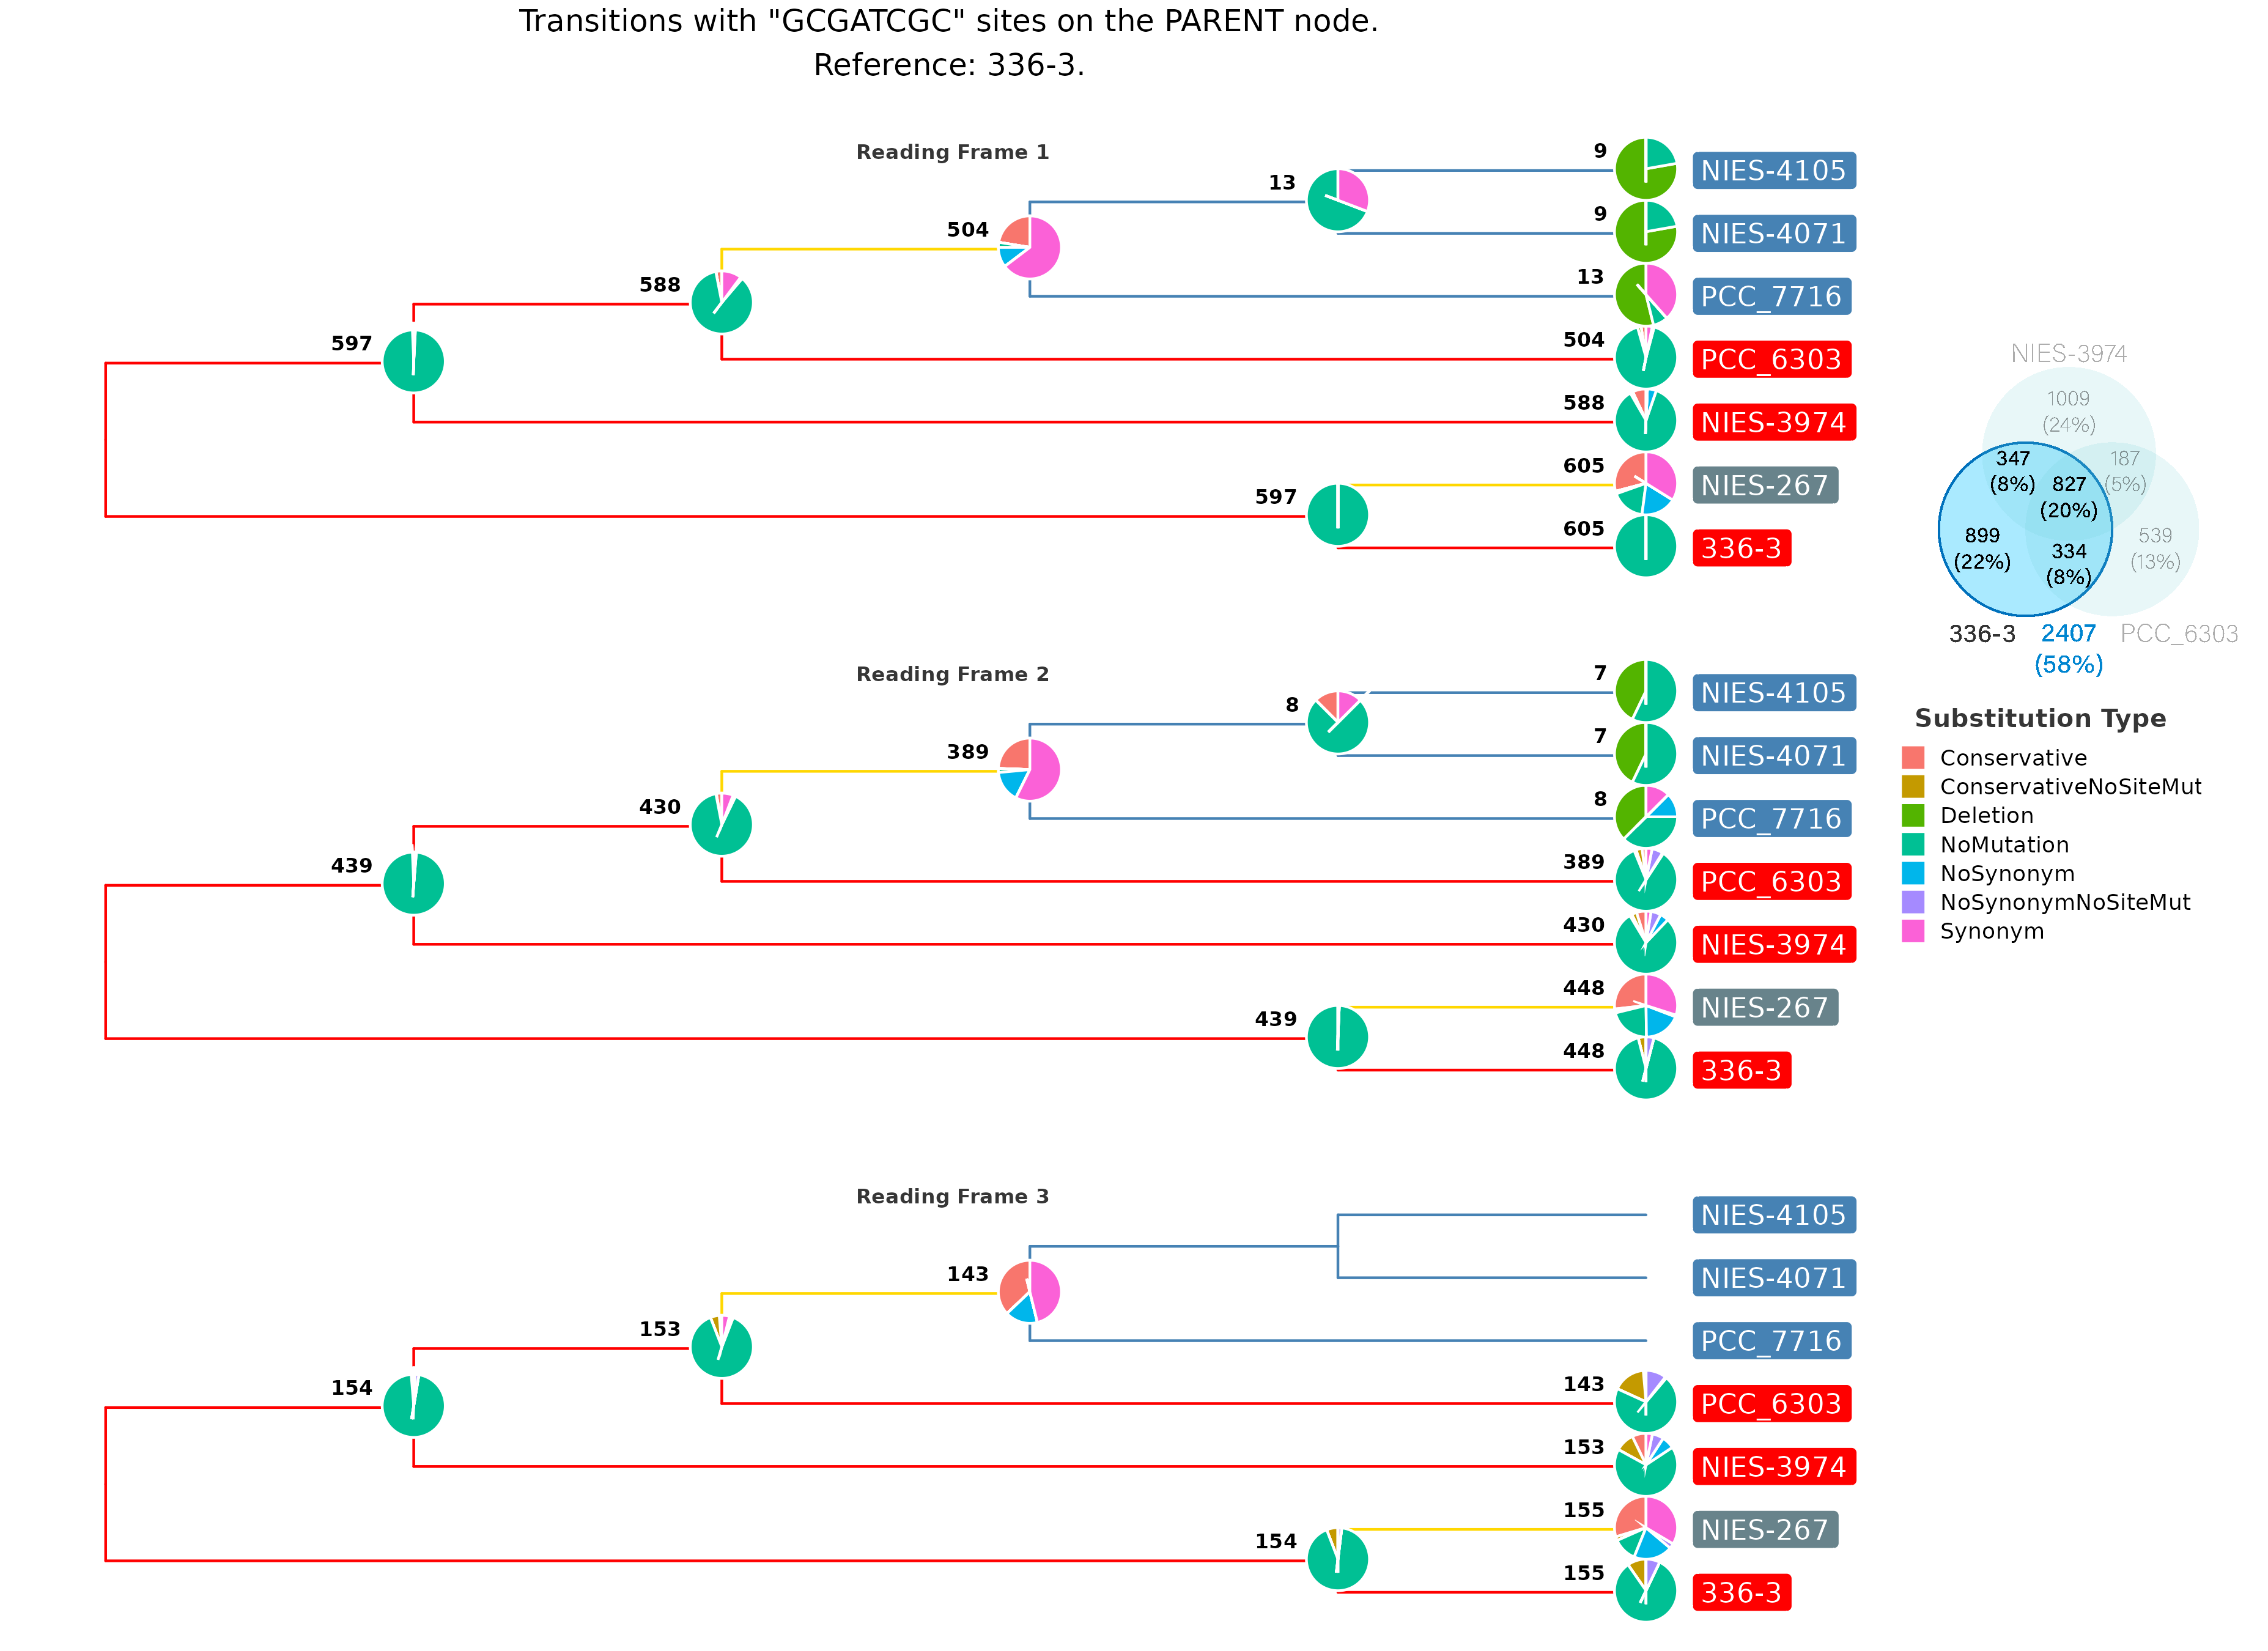
\includegraphics[width=1.2\linewidth]{Clados/Calothrix_B/figures/A/GCGATCGC/Ancestor/336-3_Ancestor_A_tree} 

}

\caption{**Conjuntos de sitios de la especie 336-3 en el conjunto ANCESTOR.** En esta figura podemos ver la filogenia anotada para los sitios de la especie 336-3, en cada nodo hay un diagrama de pie que muestra la proporcion de tipos de cambios en los aminoacidos que hubo en cada transición. Éstas proporciones se muestran para los tres marcos de lectura.}\label{fig:FIG5}
\end{figure}

\begin{figure}

{\centering 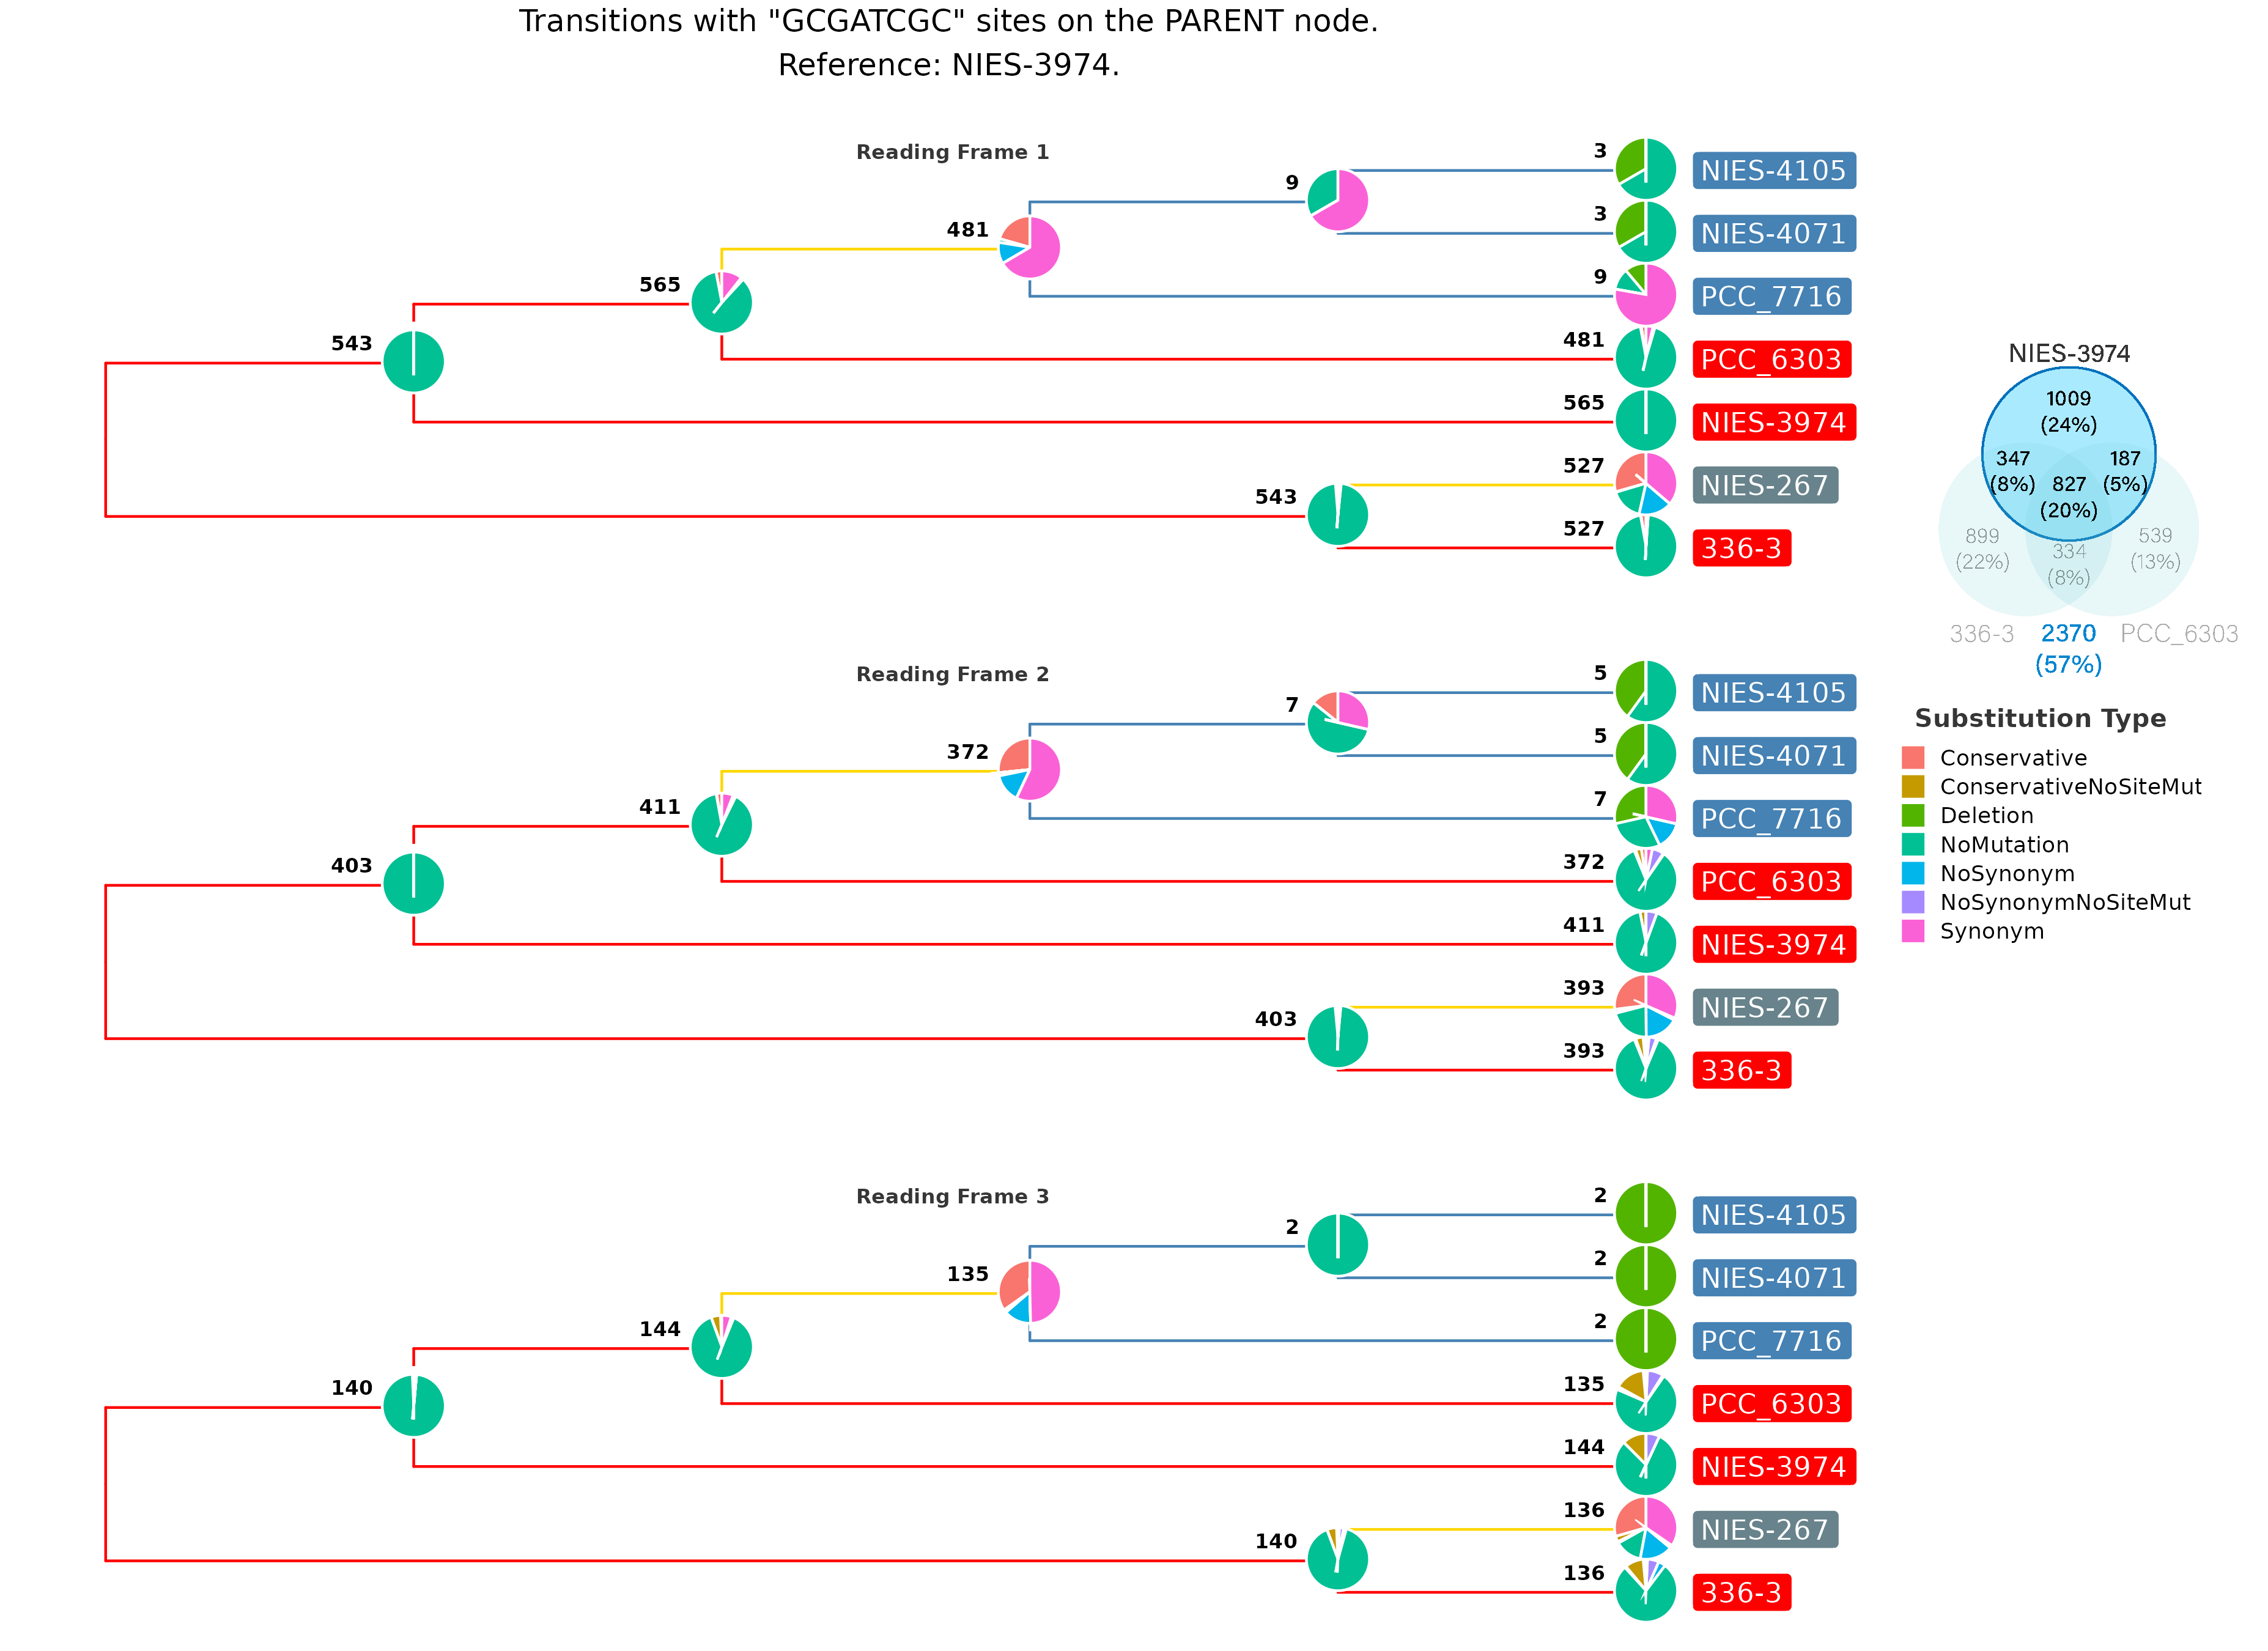
\includegraphics[width=1.2\linewidth]{Clados/Calothrix_B/figures/A/GCGATCGC/Ancestor/NIES-3974_Ancestor_A_tree} 

}

\caption{**Conjuntos de sitios de la especie NIES-3974 en el conjunto ANCESTOR.** En esta figura podemos ver la filogenia anotada para los sitios de la especie NIES-3974, en cada nodo hay un diagrama de pie que muestra la proporcion de tipos de cambios en los aminoacidos que hubo en cada transición. Éstas proporciones se muestran para los tres marcos de lectura.}\label{fig:FIG6}
\end{figure}

\begin{figure}

{\centering 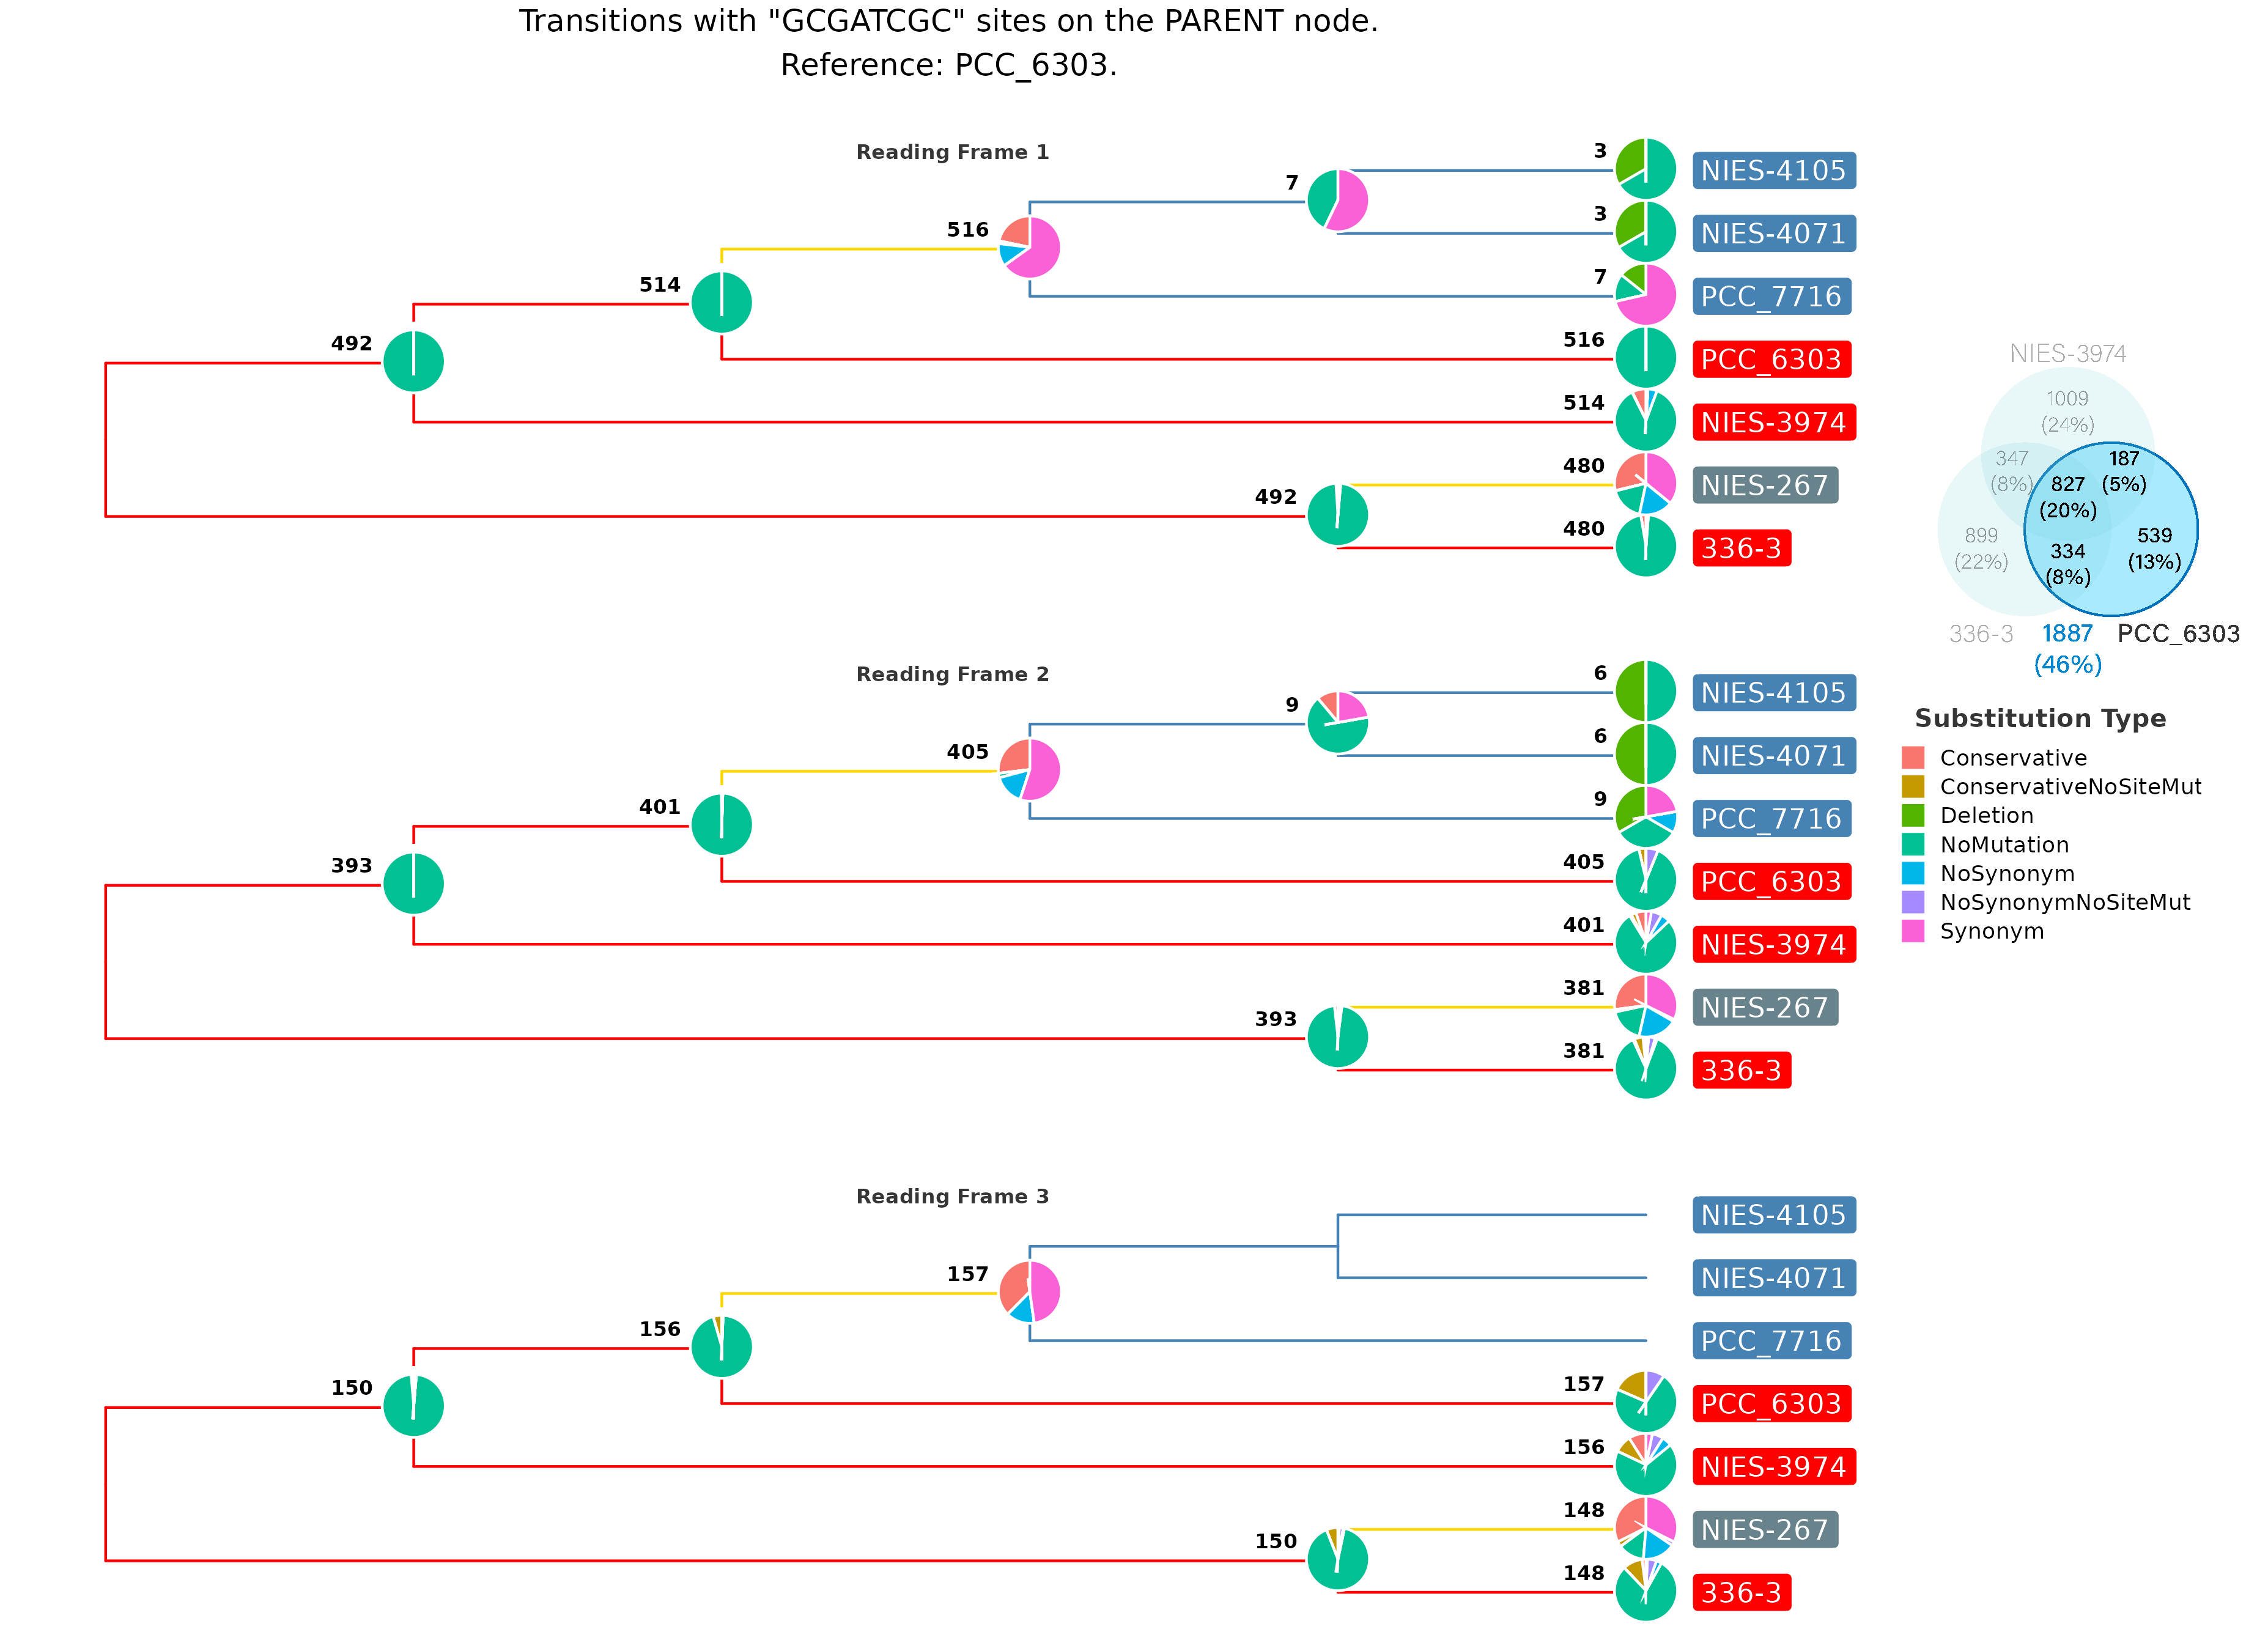
\includegraphics[width=1.2\linewidth]{Clados/Calothrix_B/figures/A/GCGATCGC/Ancestor/PCC_6303_Ancestral_A_tree} 

}

\caption{**Conjuntos de sitios de la especie PCC\_6303 en el conjunto ANCESTOR.** En esta figura podemos ver la filogenia anotada para los sitios de la especie PCC\_6303, en cada nodo hay un diagrama de pie que muestra la proporcion de tipos de cambios en los aminoacidos que hubo en cada transición. Éstas proporciones se muestran para los tres marcos de lectura.}\label{fig:FIG7}
\end{figure}

\begin{figure}

{\centering 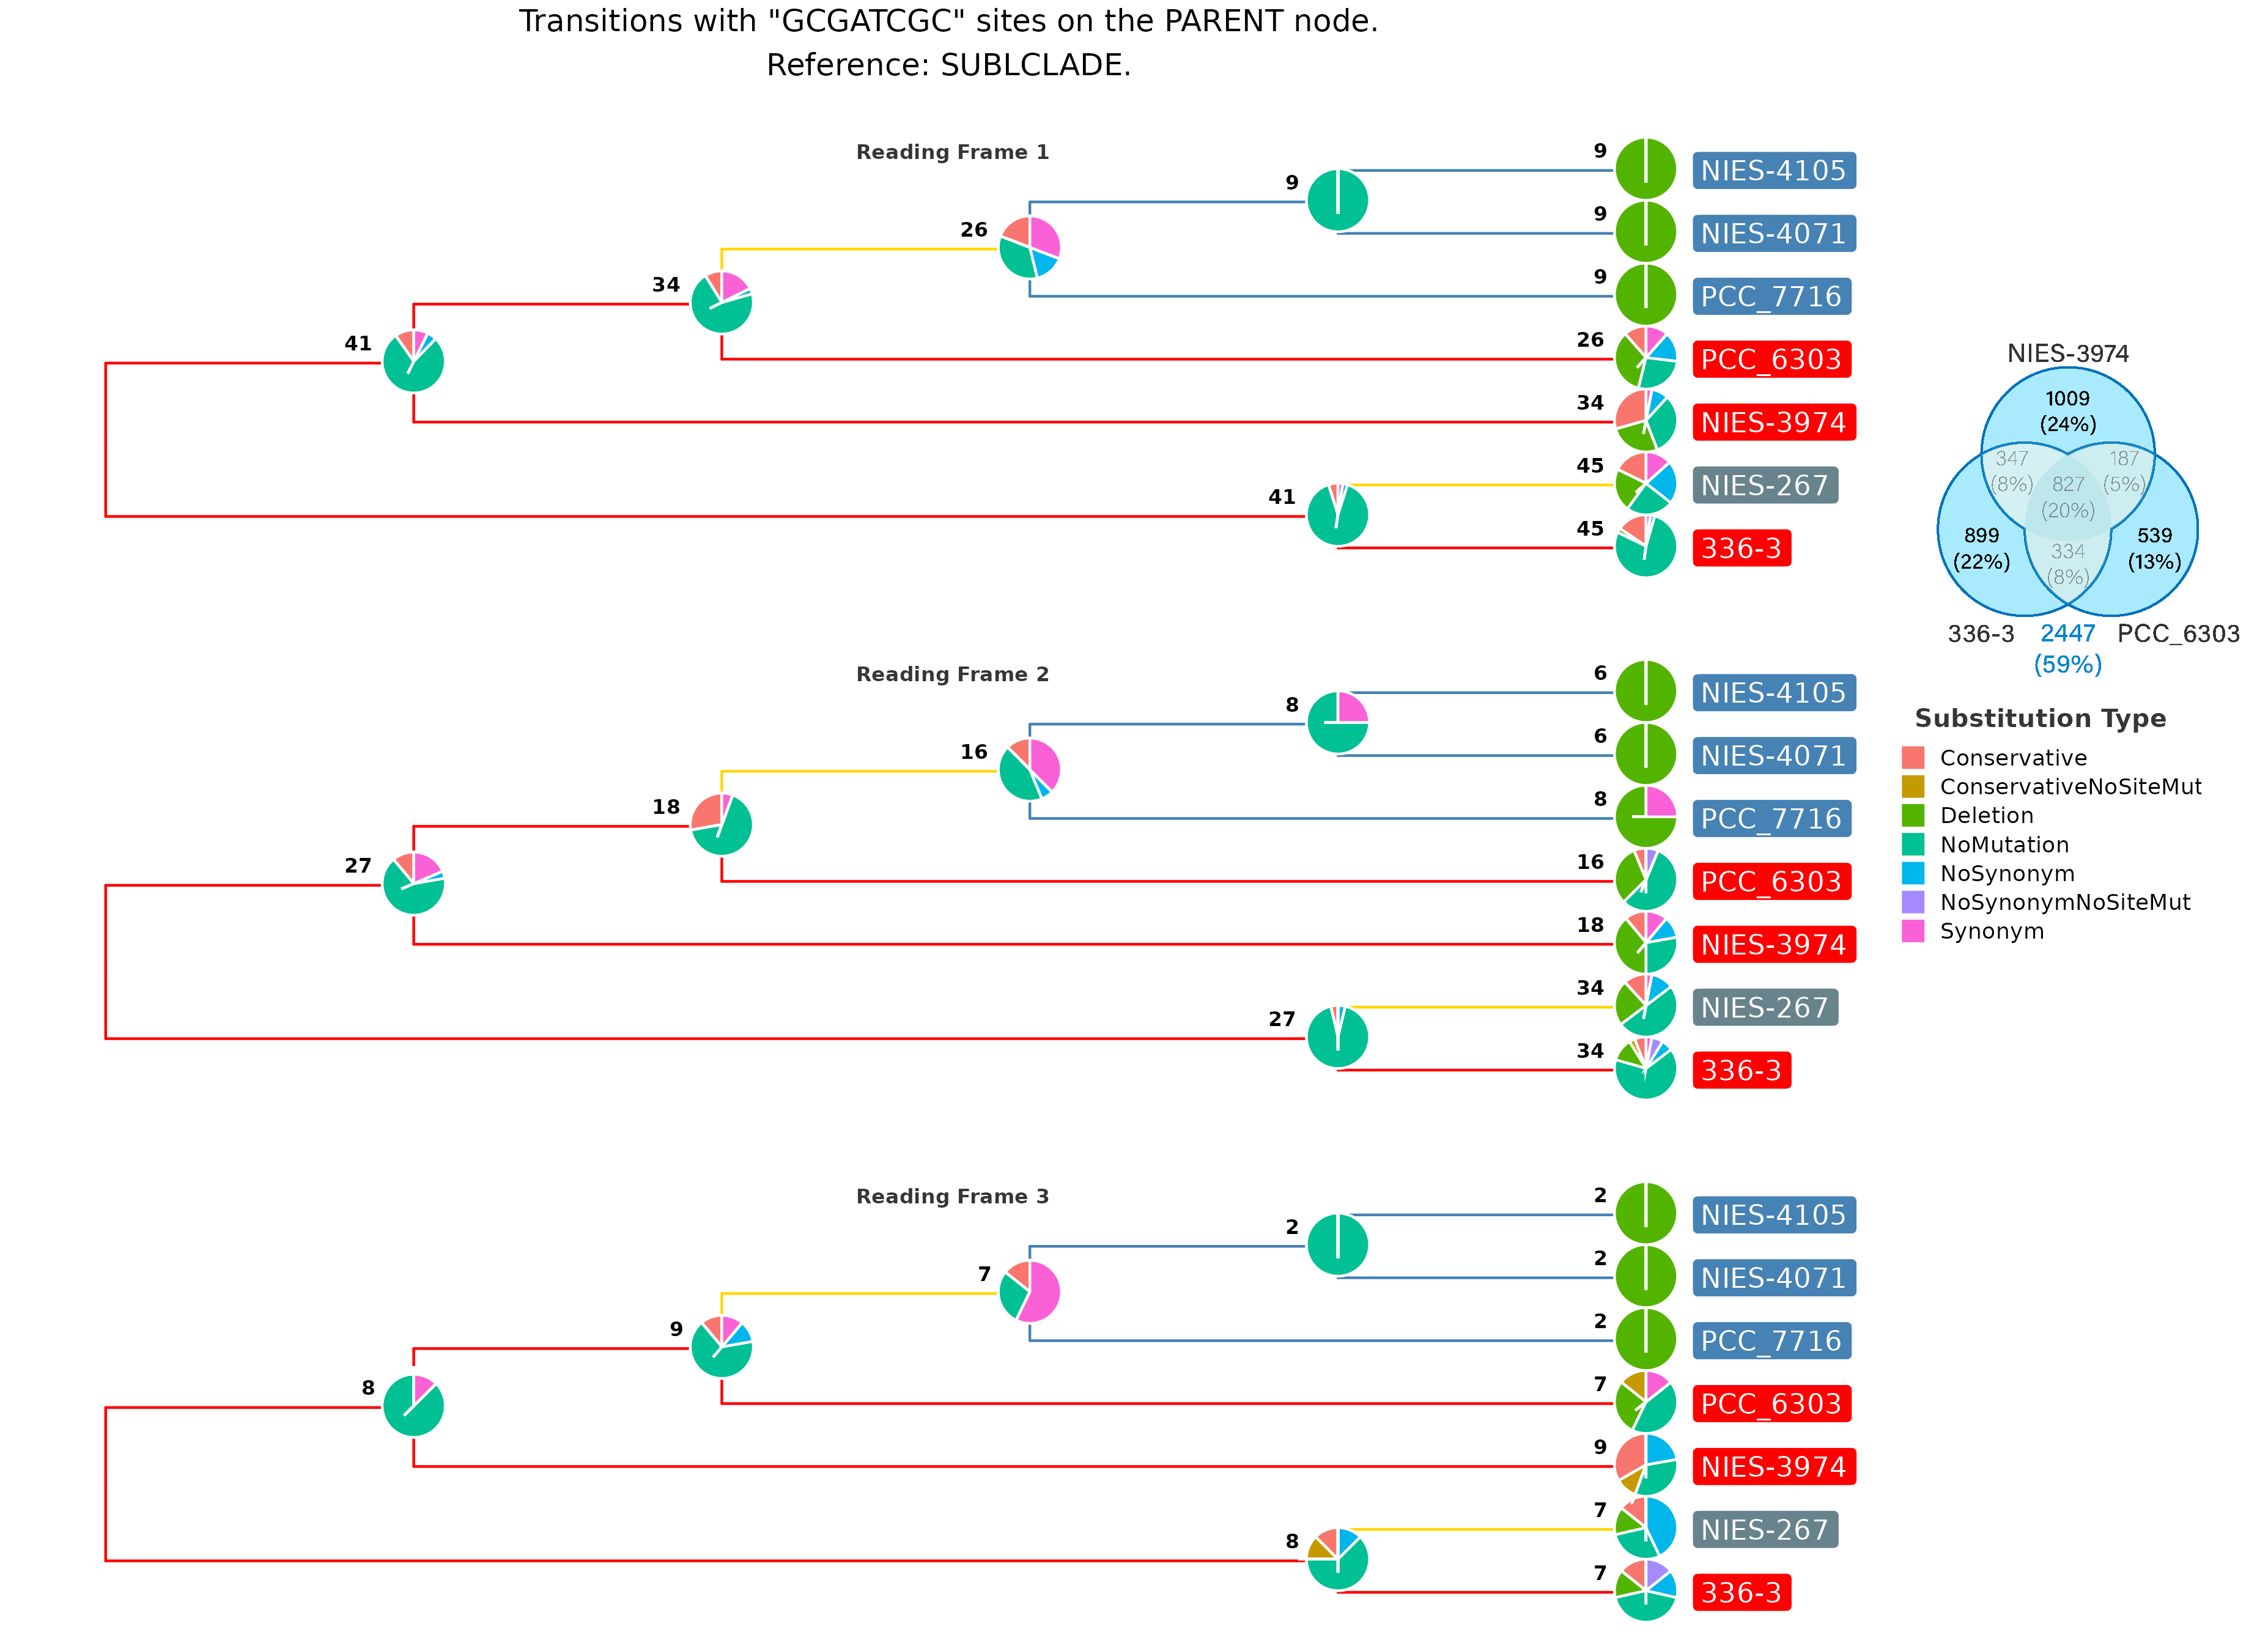
\includegraphics[width=1.2\linewidth]{Clados/Calothrix_B/figures/A/GCGATCGC/Ancestor/SUBCLADE_Ancestor_A_tree} 

}

\caption{**Conjuntos de sitios unicos entre las 3 especies en el conjunto ANCESTOR.** En esta figura podemos ver la filogenia anotada para todos los sitios unicos entre las 3 especies. En cada nodo hay un diagrama de pie que muestra la proporcion de tipos de cambios en los aminoacidos que hubo en cada transición. Éstas proporciones se muestran para los tres marcos de lectura.}\label{fig:FIG8}
\end{figure}

\hypertarget{conjunto-actual}{%
\section{Conjunto Actual}\label{conjunto-actual}}

En las *\textbf{figuras 9 a 12} se muestran los resultados del conjunto Actual, es decir transiciones que partieron de un sitio que no era \textbf{GCGATCGC} y se convirtieron en \textbf{GCGATCGC}.

En la Figura \ref{fig:FIG9} podemos ver por ejemplo que la especie \textbf{336-3} en el marco de lectura uno ganó \textbf{685} sitios \textbf{GCGATCGC} a partir de sitios que anteriormente no lo eran, esto principalmente a través de cambios no sinónimos y en menor medida a través de cambios sinónimos. Esto se observa también en los demás conjuntos (\textbf{figuras} \ref{fig:FIG10},\ref{fig:FIG11} y\ref{fig:FIG12}). Es decir en estos sitios hay una tendencia a crear esta secuencia de nucléotidos.

\begin{figure}

{\centering 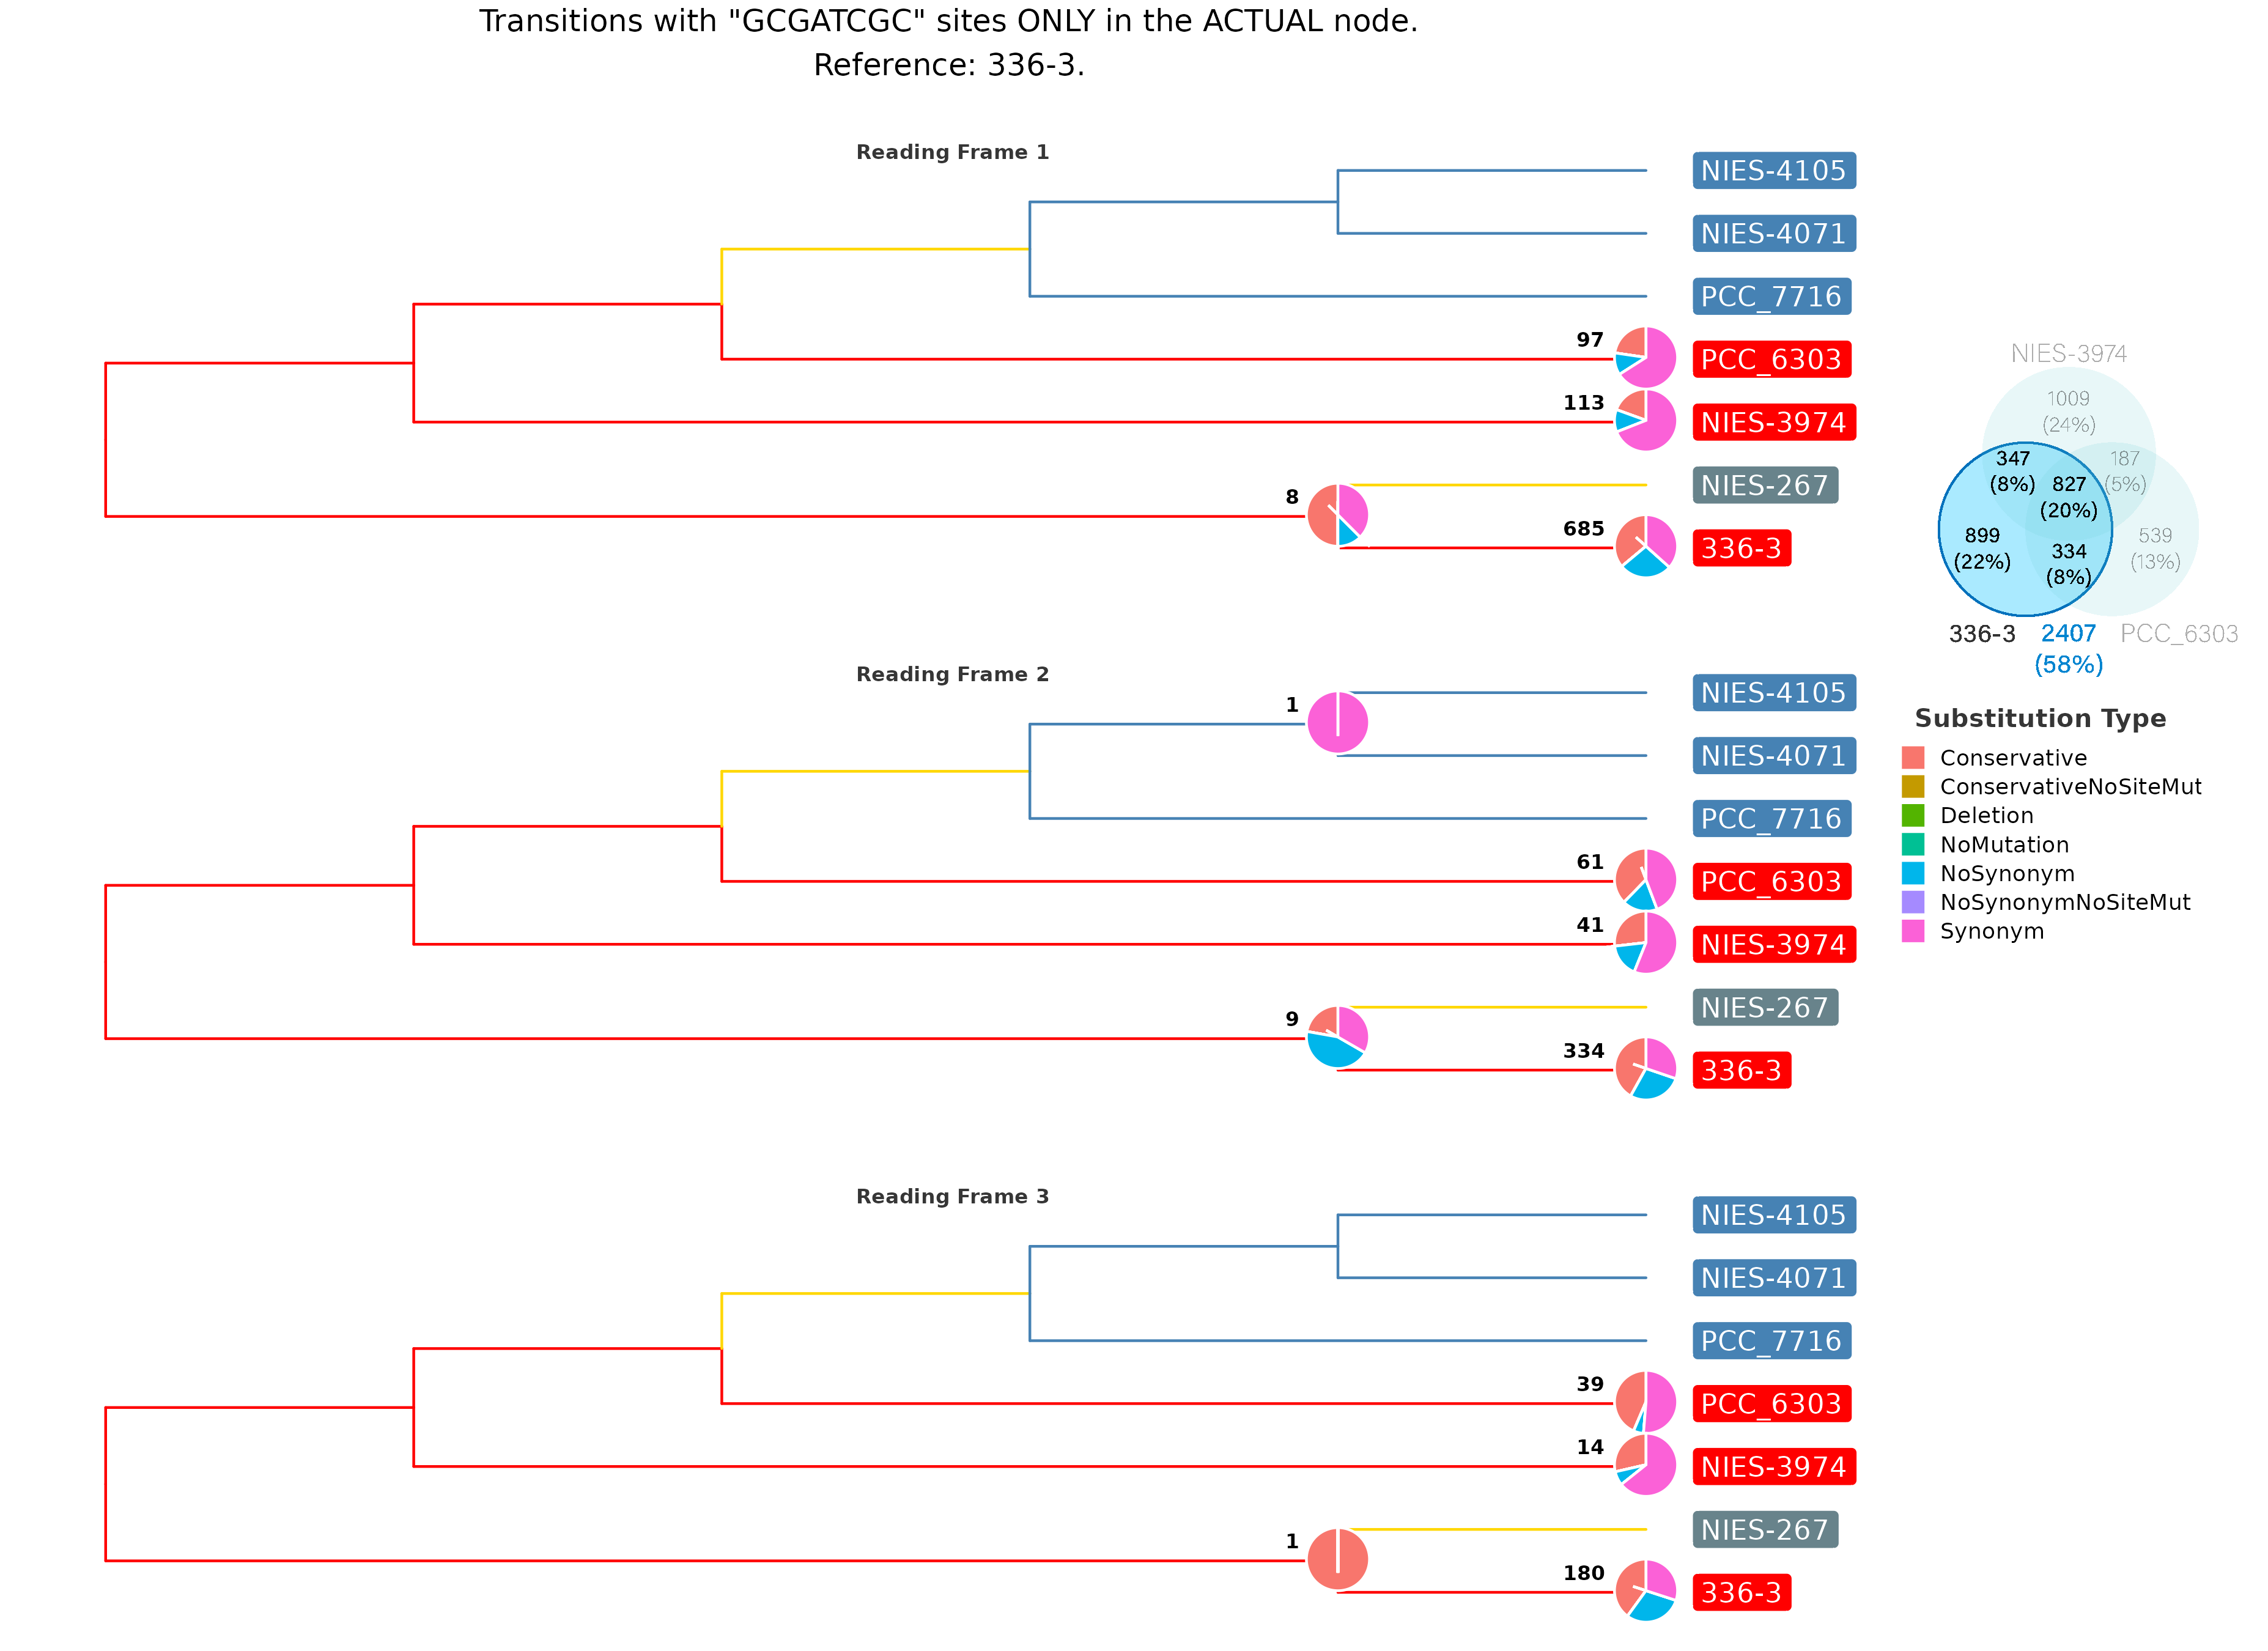
\includegraphics[width=1.2\linewidth]{Clados/Calothrix_B/figures/A/GCGATCGC/Actual/336-3_Actual_A_tree} 

}

\caption{**Conjuntos de sitios de la especie 336-3 en el conjunto ACTUAL.** En esta figura podemos ver la filogenia anotada para los sitios de la especie 336-3, en cada nodo hay un diagrama de pie que muestra la proporcion de tipos de cambios en los aminoacidos que hubo en cada transición. Éstas proporciones se muestran para los tres marcos de lectura.}\label{fig:FIG9}
\end{figure}

\begin{figure}

{\centering 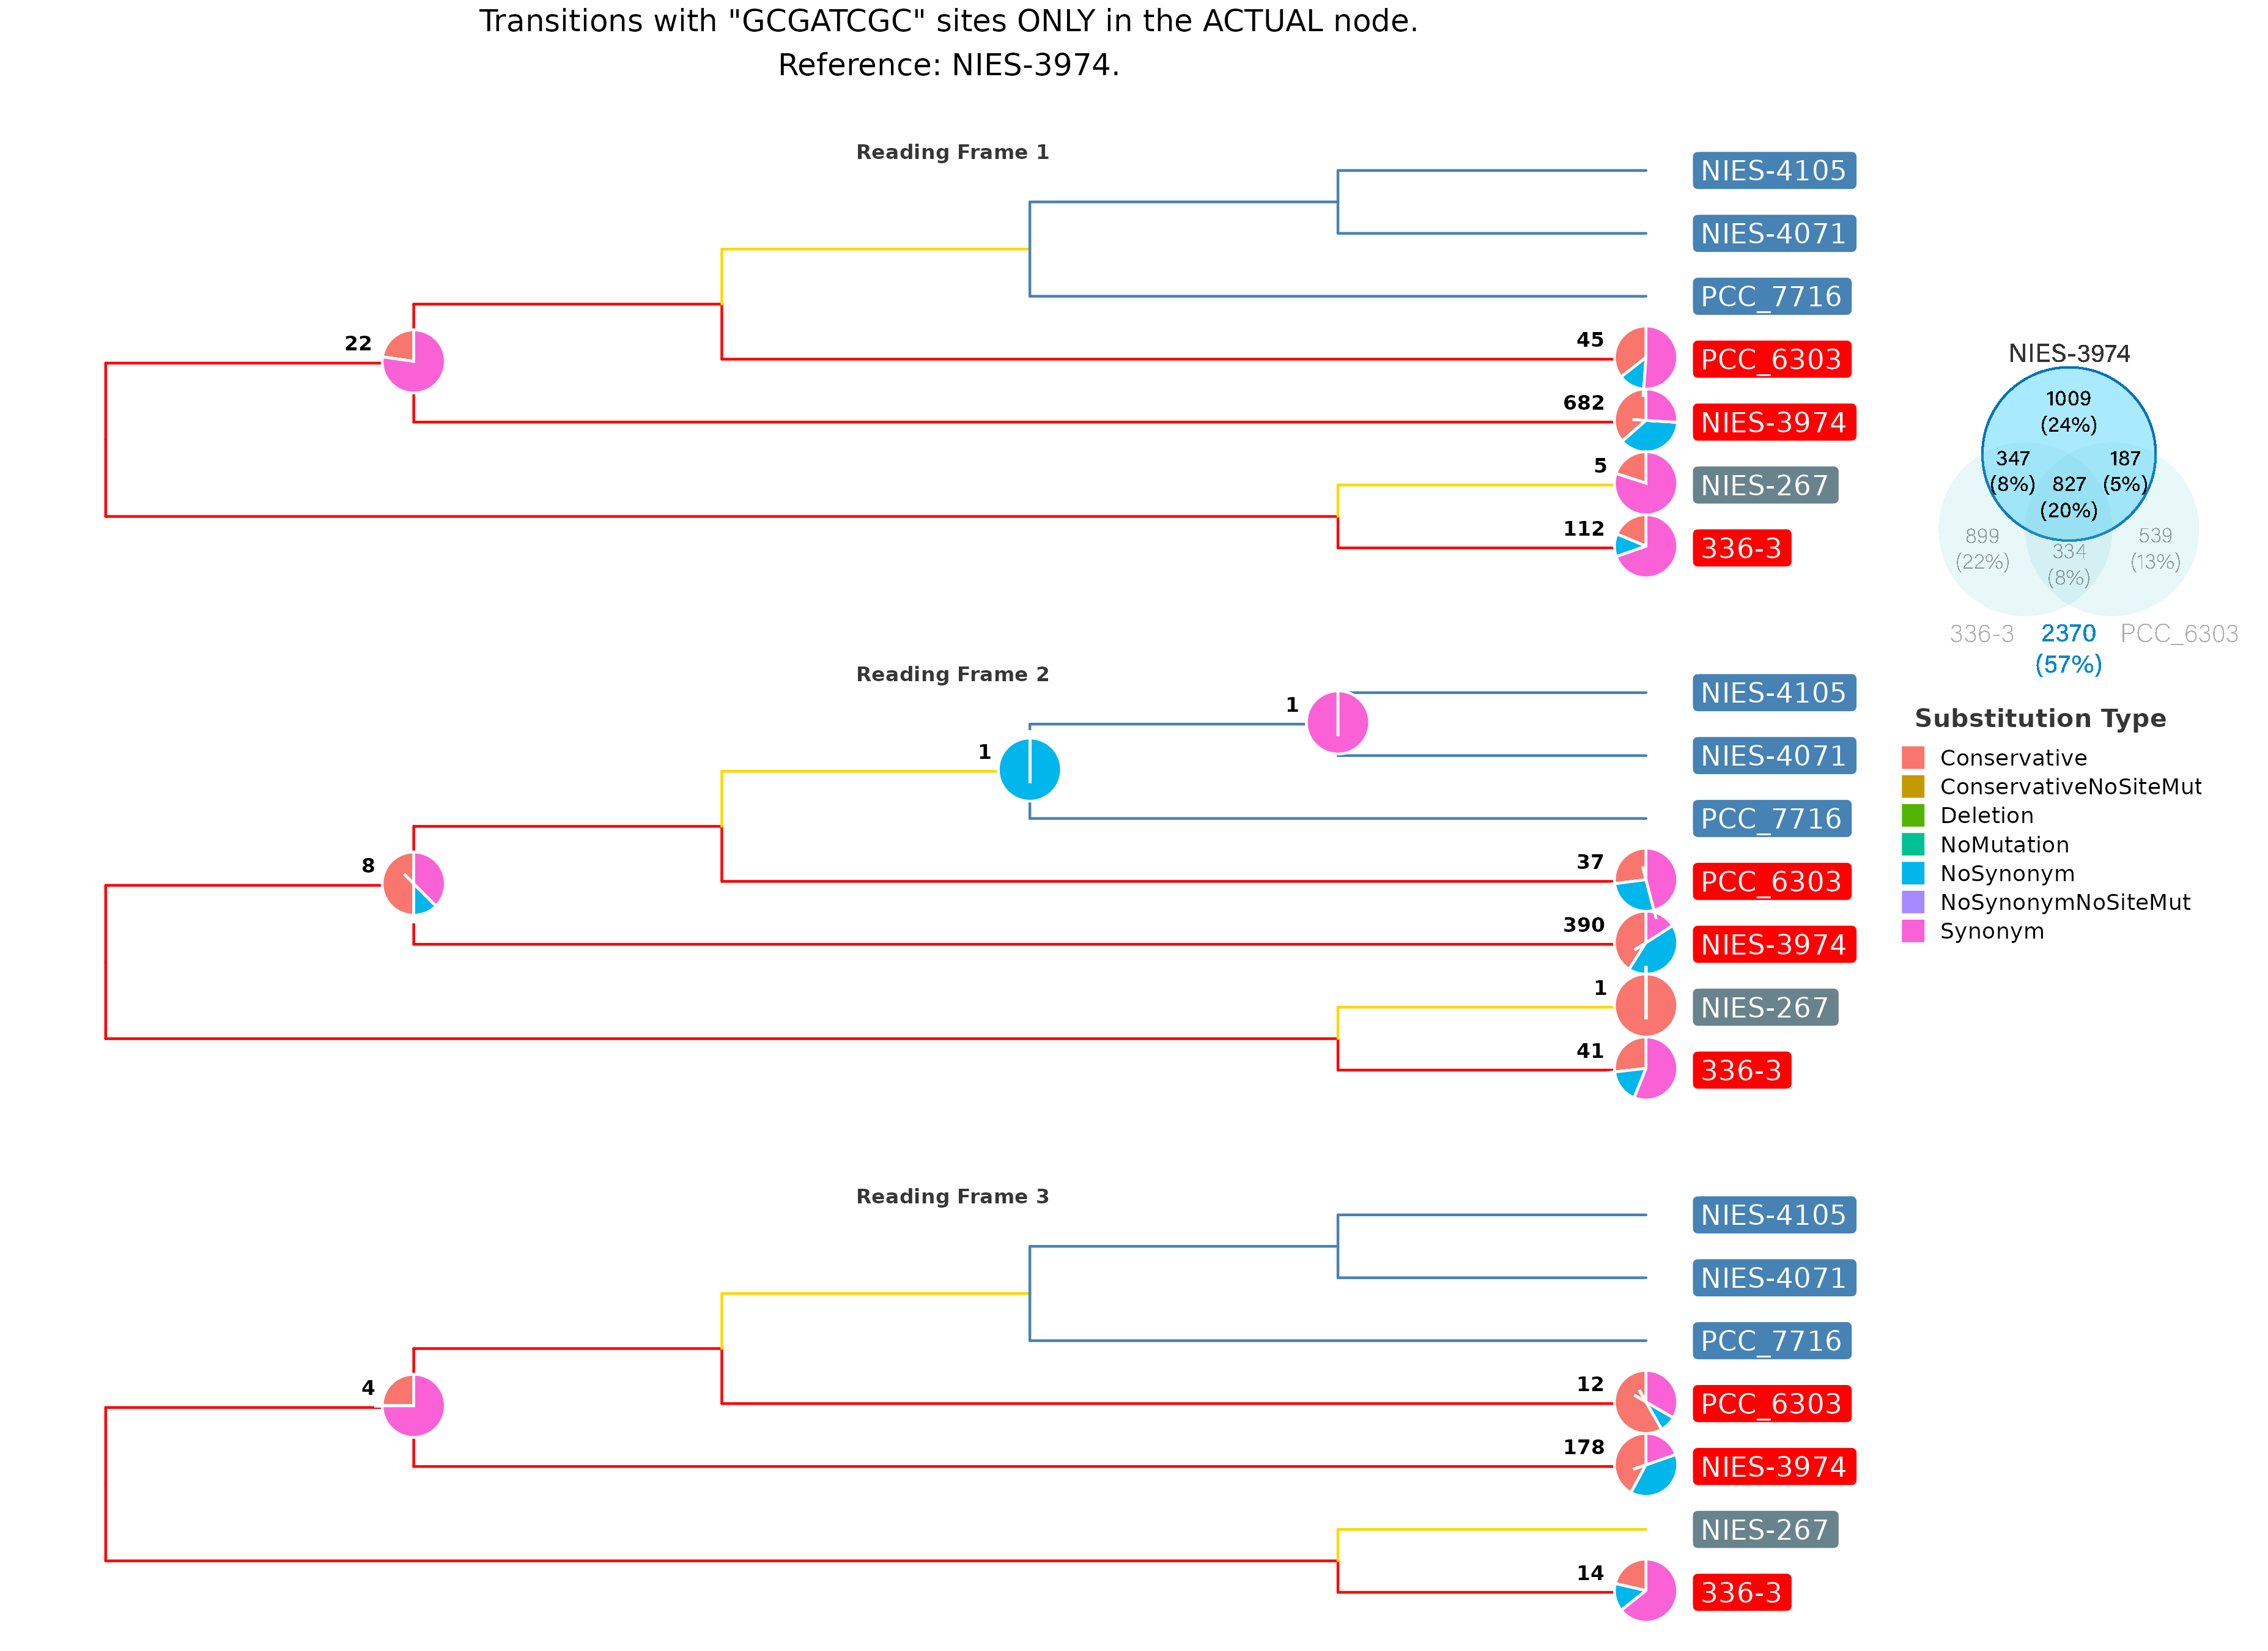
\includegraphics[width=1.2\linewidth]{Clados/Calothrix_B/figures/A/GCGATCGC/Actual/NIES-3974_Actual_A_tree} 

}

\caption{**Conjuntos de sitios de la especie NIES-3974 en el conjunto ACTUAL.** En esta figura podemos ver la filogenia anotada para los sitios de la especie NIES-3974, en cada nodo hay un diagrama de pie que muestra la proporcion de tipos de cambios en los aminoacidos que hubo en cada transición. Éstas proporciones se muestran para los tres marcos de lectura.}\label{fig:FIG10}
\end{figure}

\begin{figure}

{\centering 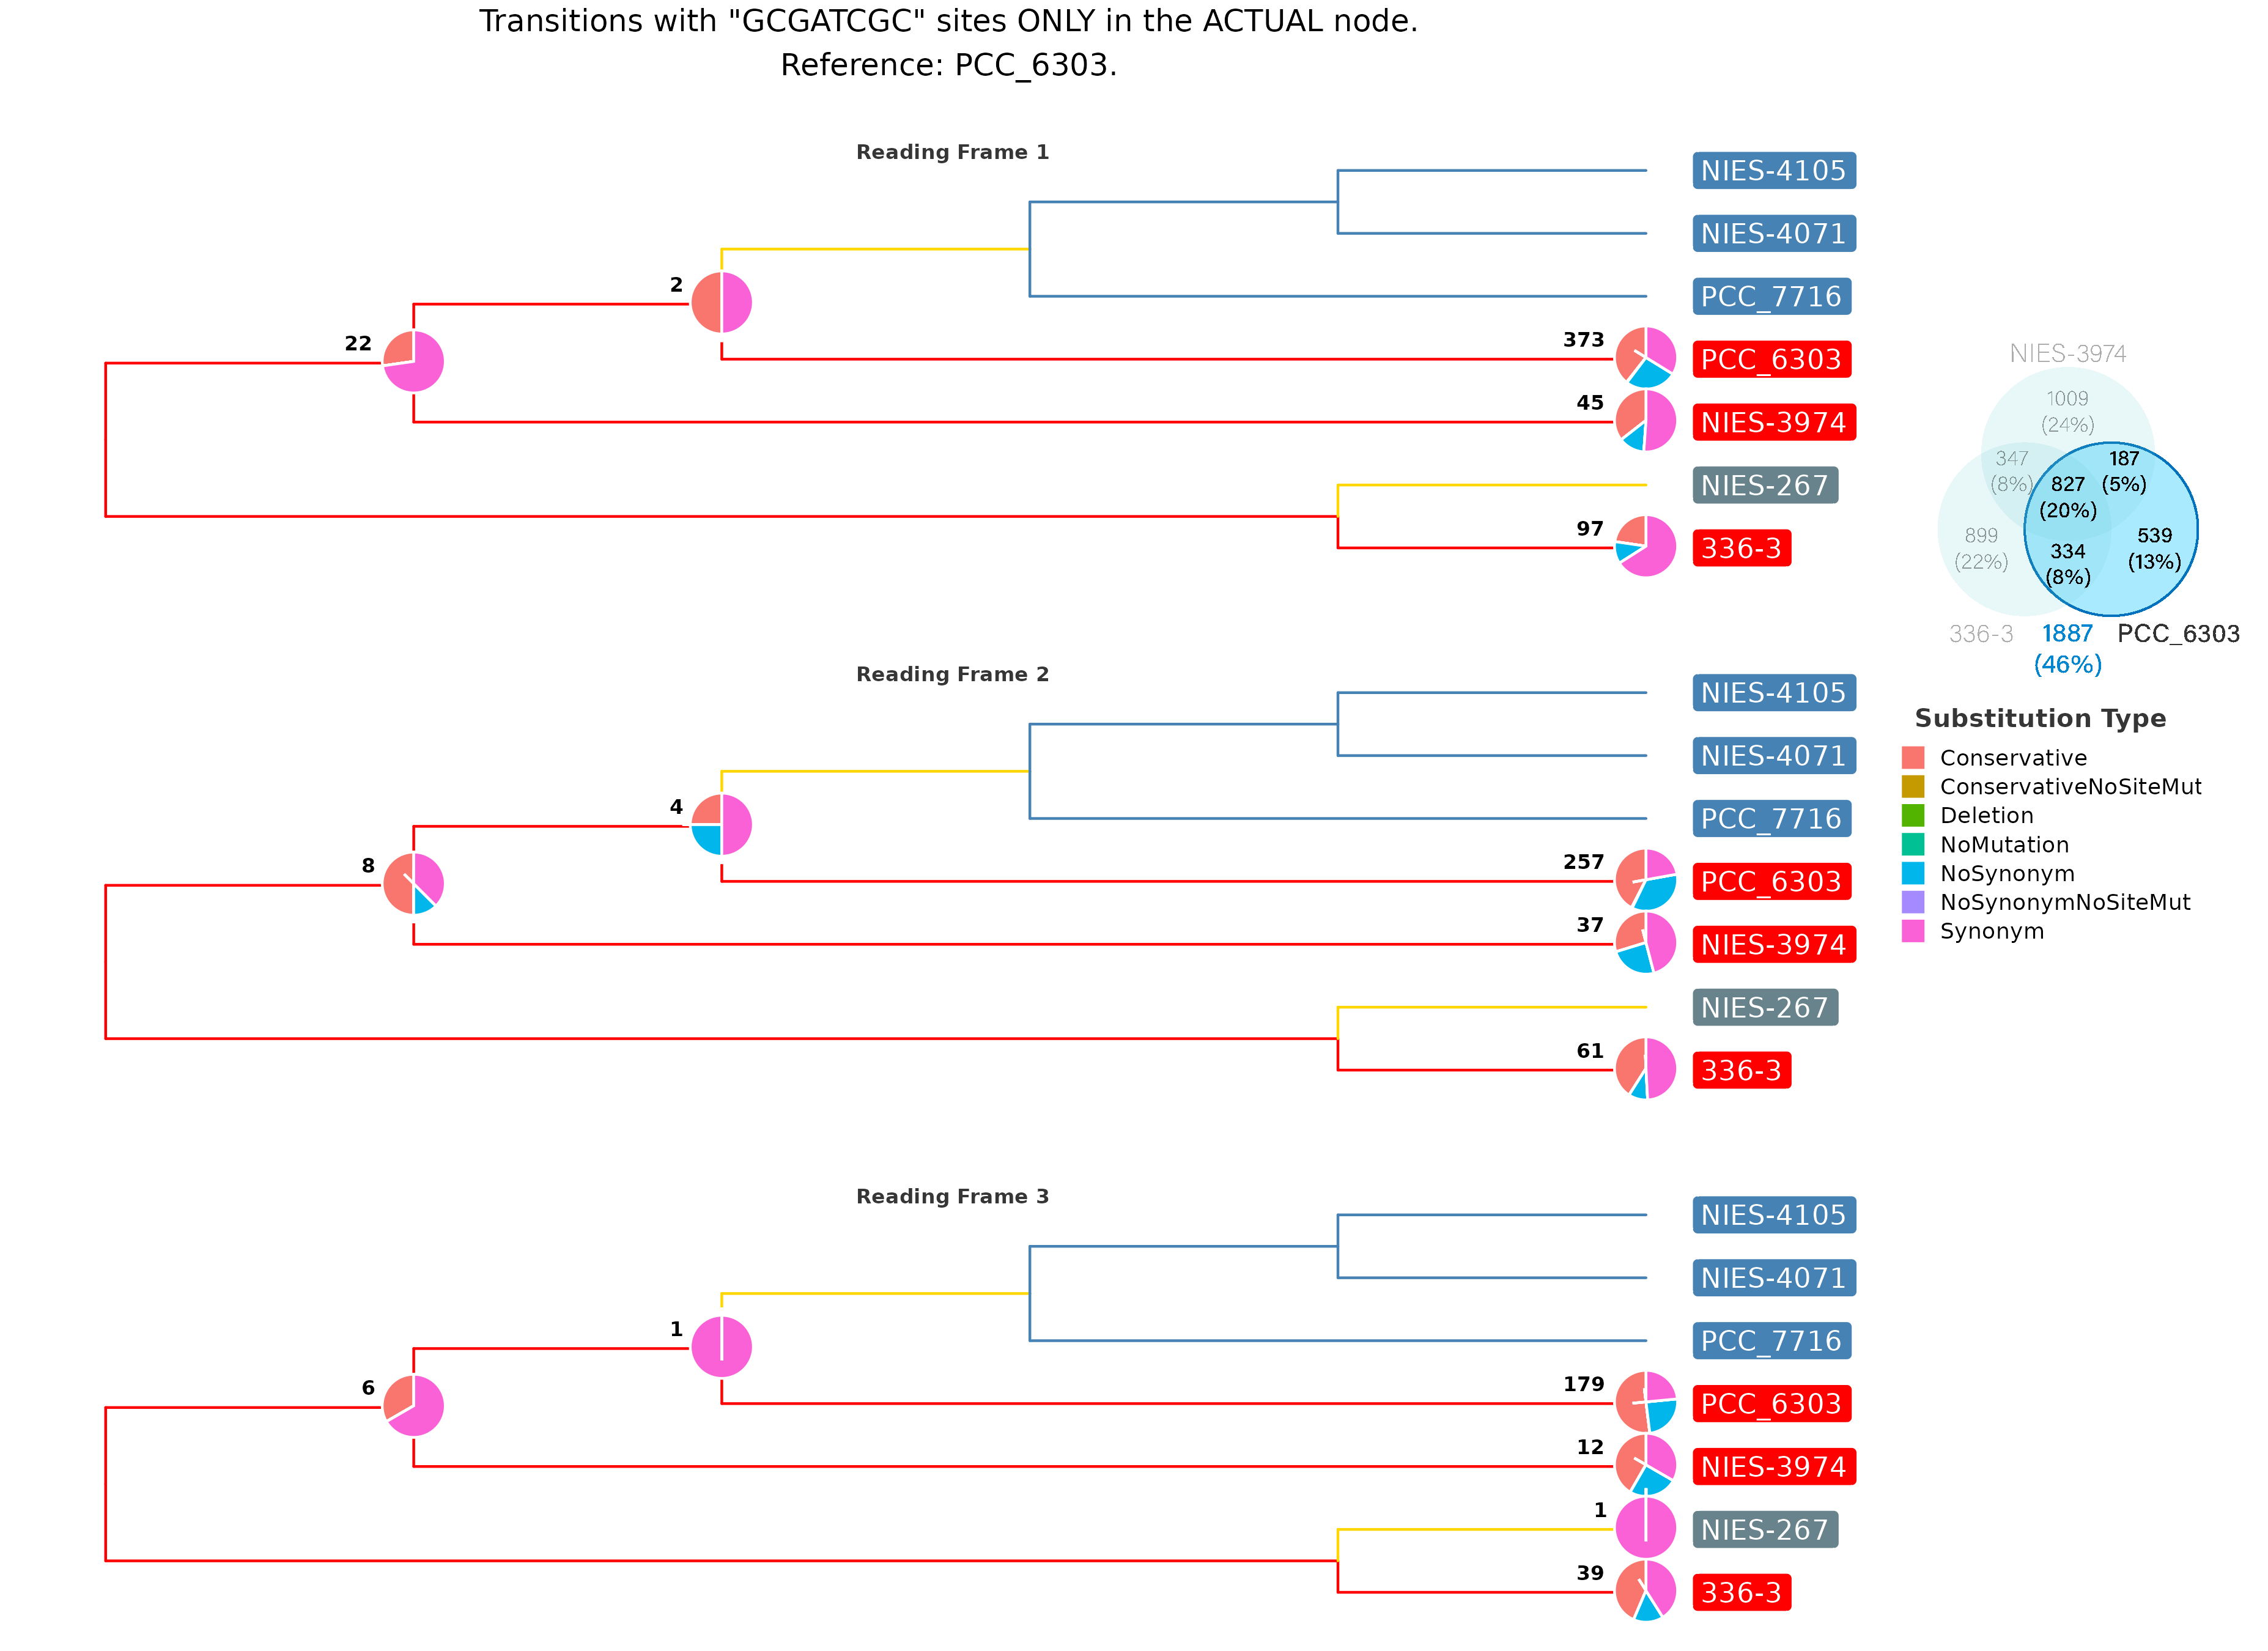
\includegraphics[width=1.2\linewidth]{Clados/Calothrix_B/figures/A/GCGATCGC/Actual/PCC_6303_Actual_A_tree} 

}

\caption{**Conjuntos de sitios de la especie PCC\_6303 en el conjunto ACTUAL.** En esta figura podemos ver la filogenia anotada para los sitios de la especie PCC\_6303, en cada nodo hay un diagrama de pie que muestra la proporcion de tipos de cambios en los aminoacidos que hubo en cada transición. Éstas proporciones se muestran para los tres marcos de lectura.}\label{fig:FIG11}
\end{figure}

\begin{figure}

{\centering 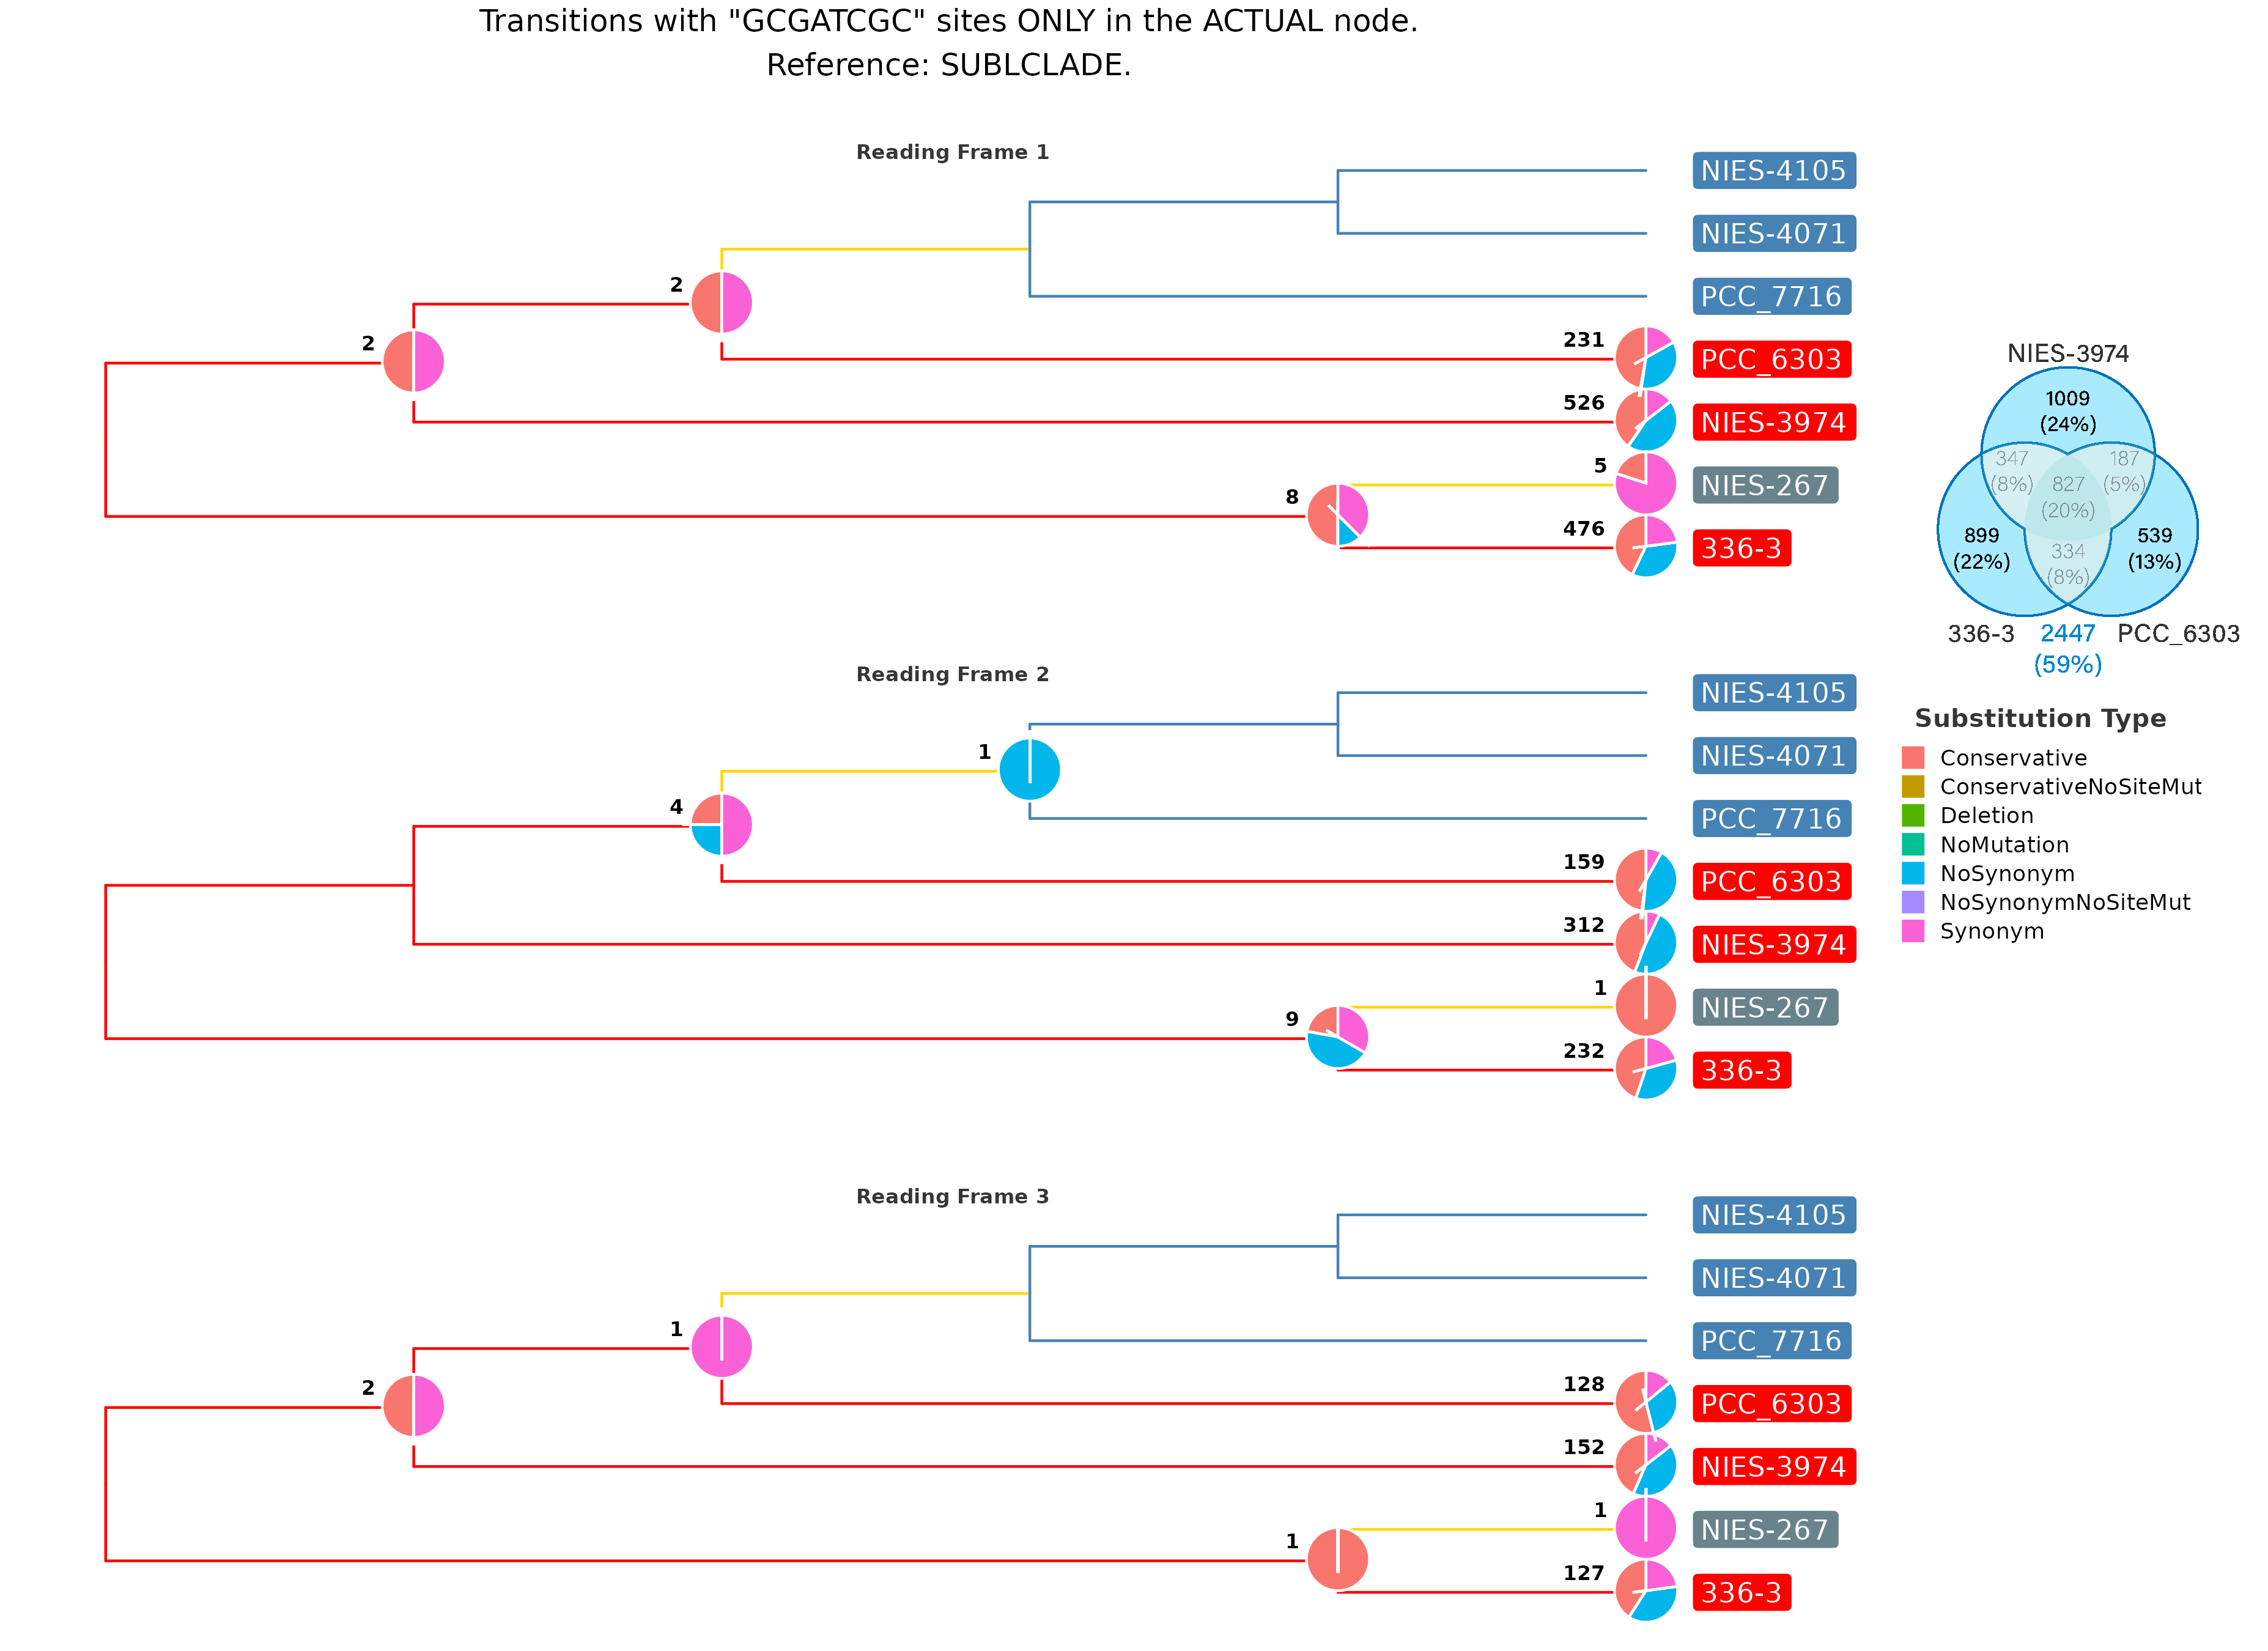
\includegraphics[width=1.2\linewidth]{Clados/Calothrix_B/figures/A/GCGATCGC/Actual/SUBCLADE_Actual_A_tree} 

}

\caption{**Conjuntos de sitios unicos entre las 3 especies en el conjunto ACTUAL.** En esta figura podemos ver la filogenia anotada para todos los sitios unicos entre las 3 especies. En cada nodo hay un diagrama de pie que muestra la proporcion de tipos de cambios en los aminoacidos que hubo en cada transición. Éstas proporciones se muestran para los tres marcos de lectura.}\label{fig:FIG12}
\end{figure}

\hypertarget{conjunto-all}{%
\section{Conjunto All}\label{conjunto-all}}

En las \textbf{figuras 13 a 16} se muestran los resultados del conjunto \textbf{All}, es decir todas las transiciones que ocurrieron en los sitios de la especie de referencia.

Por ejemplo, en la Figura \ref{fig:FIG13} podemos ver que en el marco de lectura hubo 1290 sitios GCGATCGC los cuales son sitios de la especie 336-3. Lo interesante de esta figura es que podemos ver que en la transición entre los nodos 9 y 10 parece ser que la mayoria de cambios son no sinónimos, y posteriormente la mayoría se conservan. Esta tendencia se observa en los demás conjuntos (\textbf{figuras} \ref{fig:FIG14},\ref{fig:FIG15} y\ref{fig:FIG16}) por lo tanto parece ser que la secuencia de aminoacidos tiende a conservarse.

\begin{figure}

{\centering 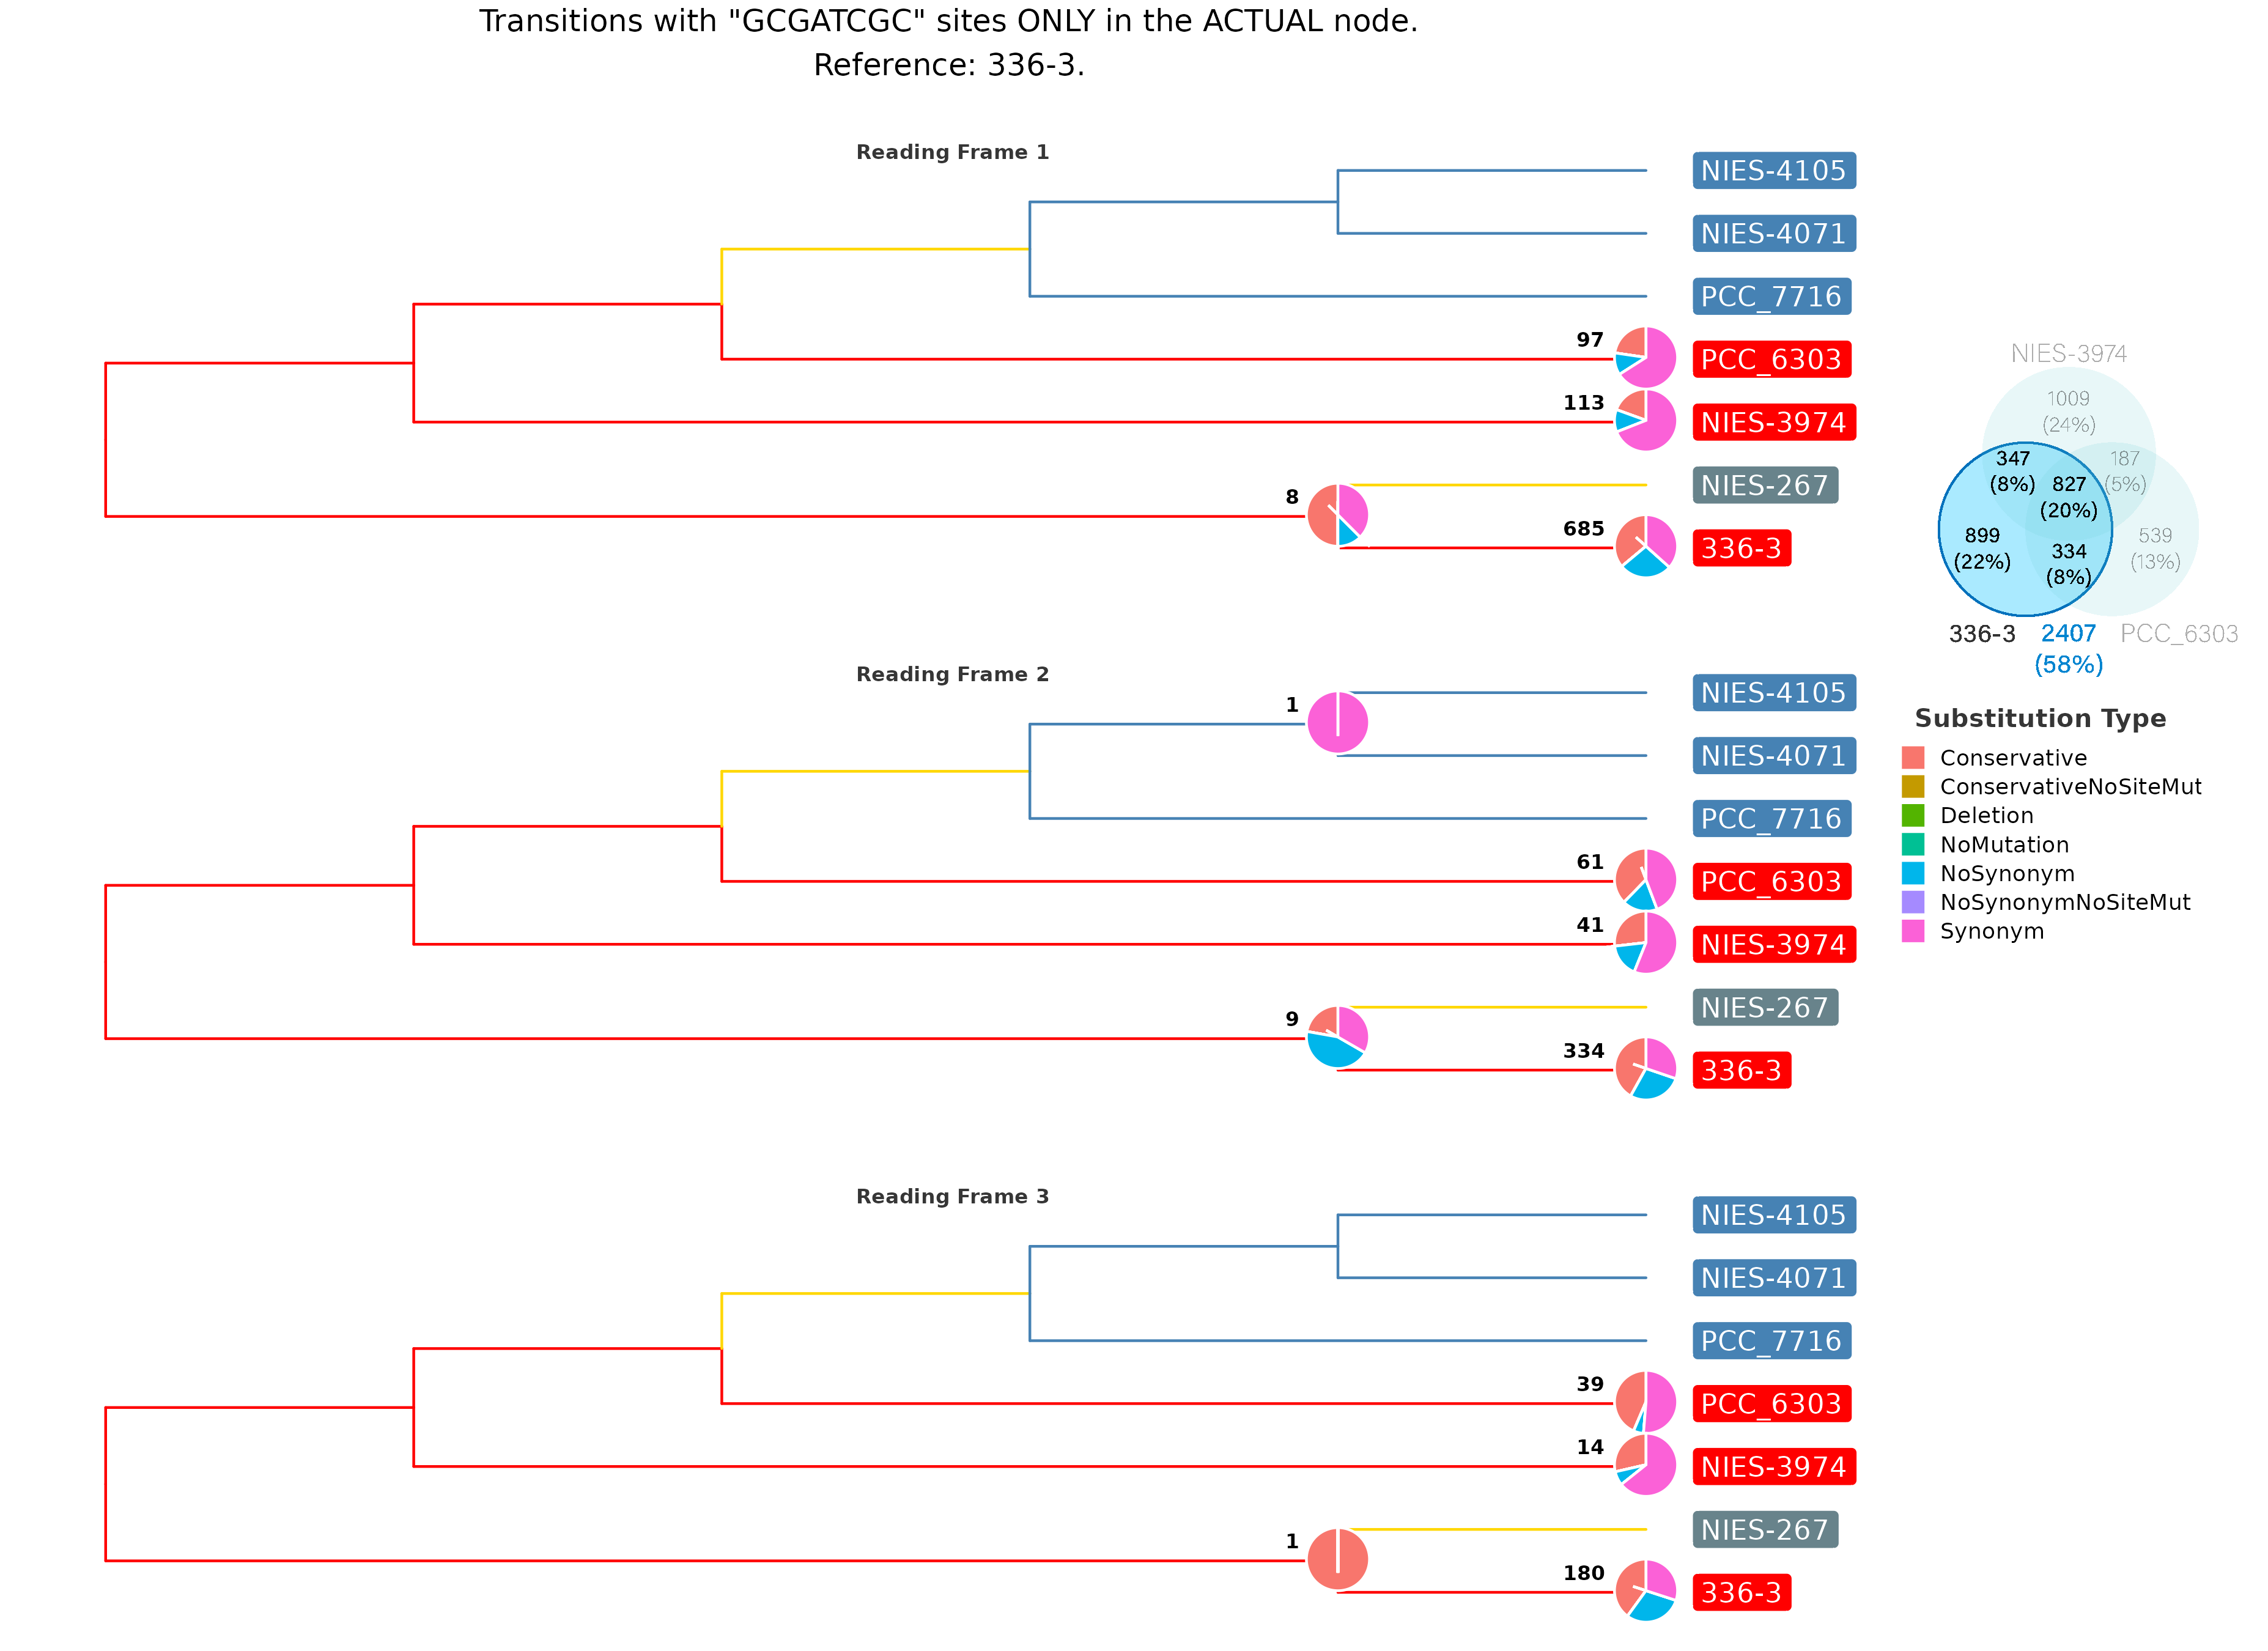
\includegraphics[width=1.2\linewidth]{Clados/Calothrix_B/figures/A/GCGATCGC/Actual/336-3_Actual_A_tree} 

}

\caption{**Conjuntos de sitios de la especie 336-3 en el conjunto ALL.** En esta figura podemos ver la filogenia anotada para los sitios de la especie 336-3, en cada nodo hay un diagrama de pie que muestra la proporcion de tipos de cambios en los aminoacidos que hubo en cada transición. Éstas proporciones se muestran para los tres marcos de lectura.}\label{fig:FIG13}
\end{figure}

\begin{figure}

{\centering 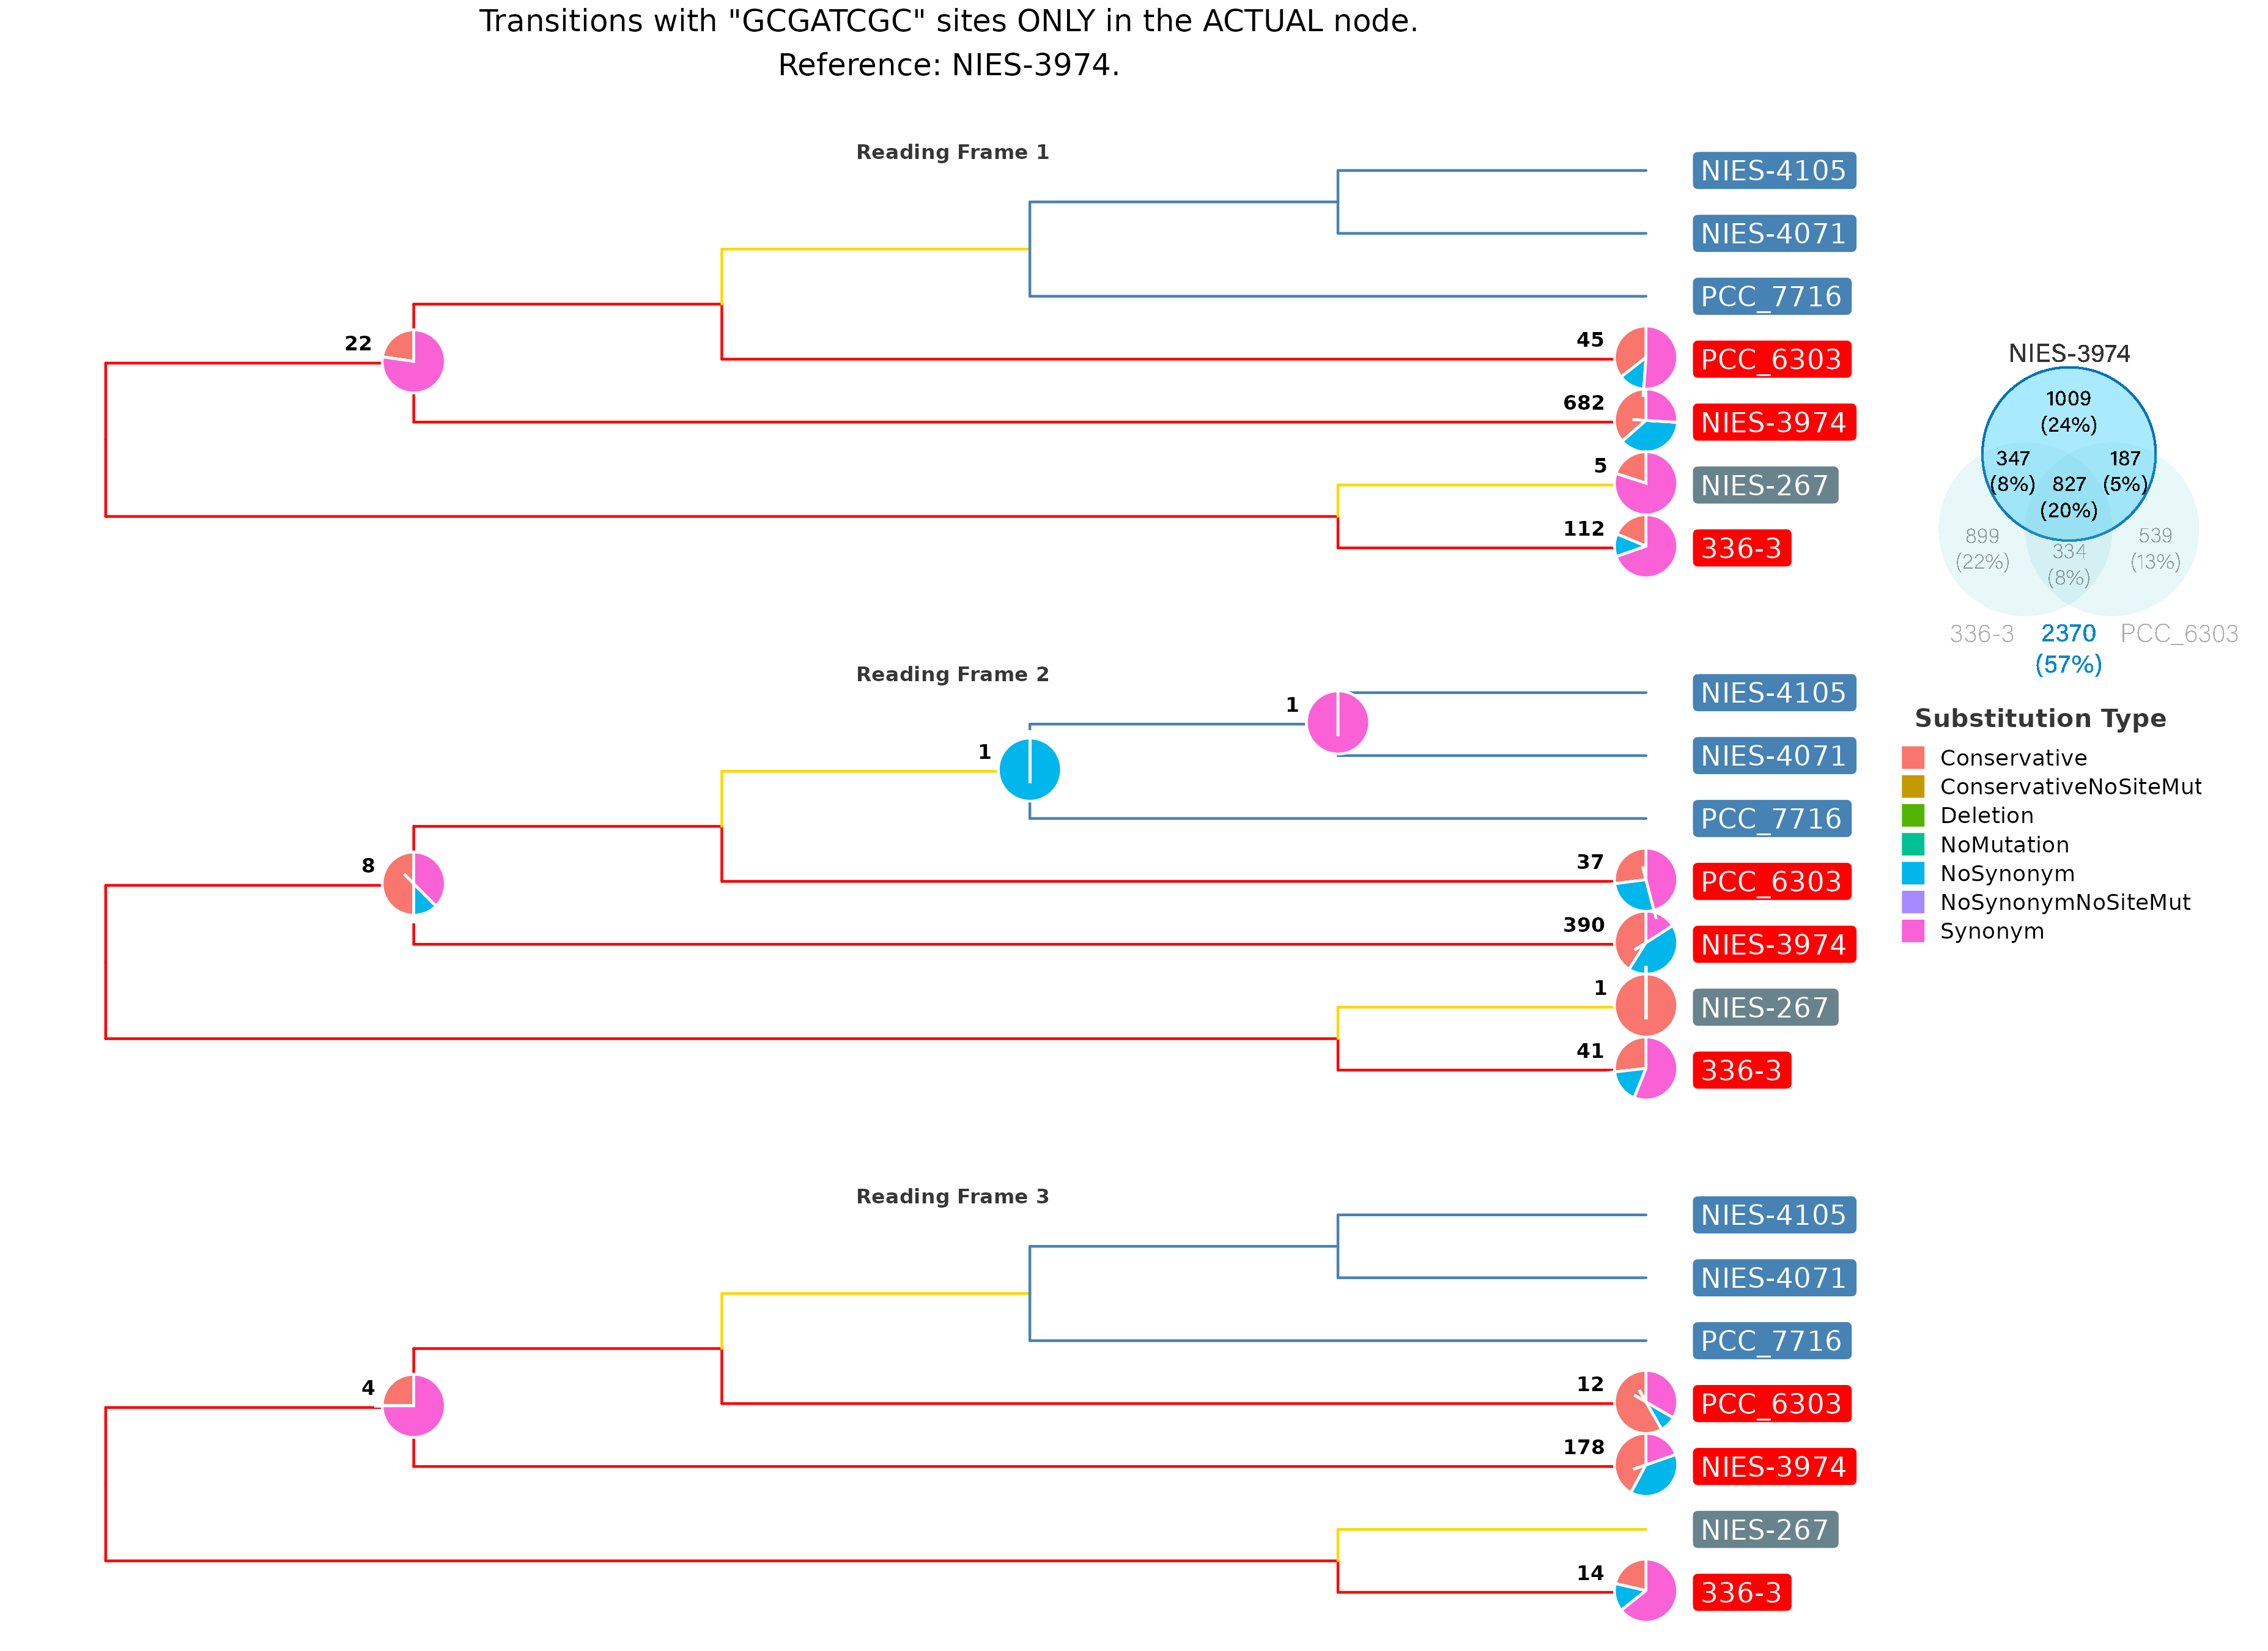
\includegraphics[width=1.2\linewidth]{Clados/Calothrix_B/figures/A/GCGATCGC/Actual/NIES-3974_Actual_A_tree} 

}

\caption{**Conjuntos de sitios de la especie NIES-3974 en el conjunto ALL.** En esta figura podemos ver la filogenia anotada para los sitios de la especie NIES-3974, en cada nodo hay un diagrama de pie que muestra la proporcion de tipos de cambios en los aminoacidos que hubo en cada transición. Éstas proporciones se muestran para los tres marcos de lectura.}\label{fig:FIG14}
\end{figure}

\begin{figure}

{\centering 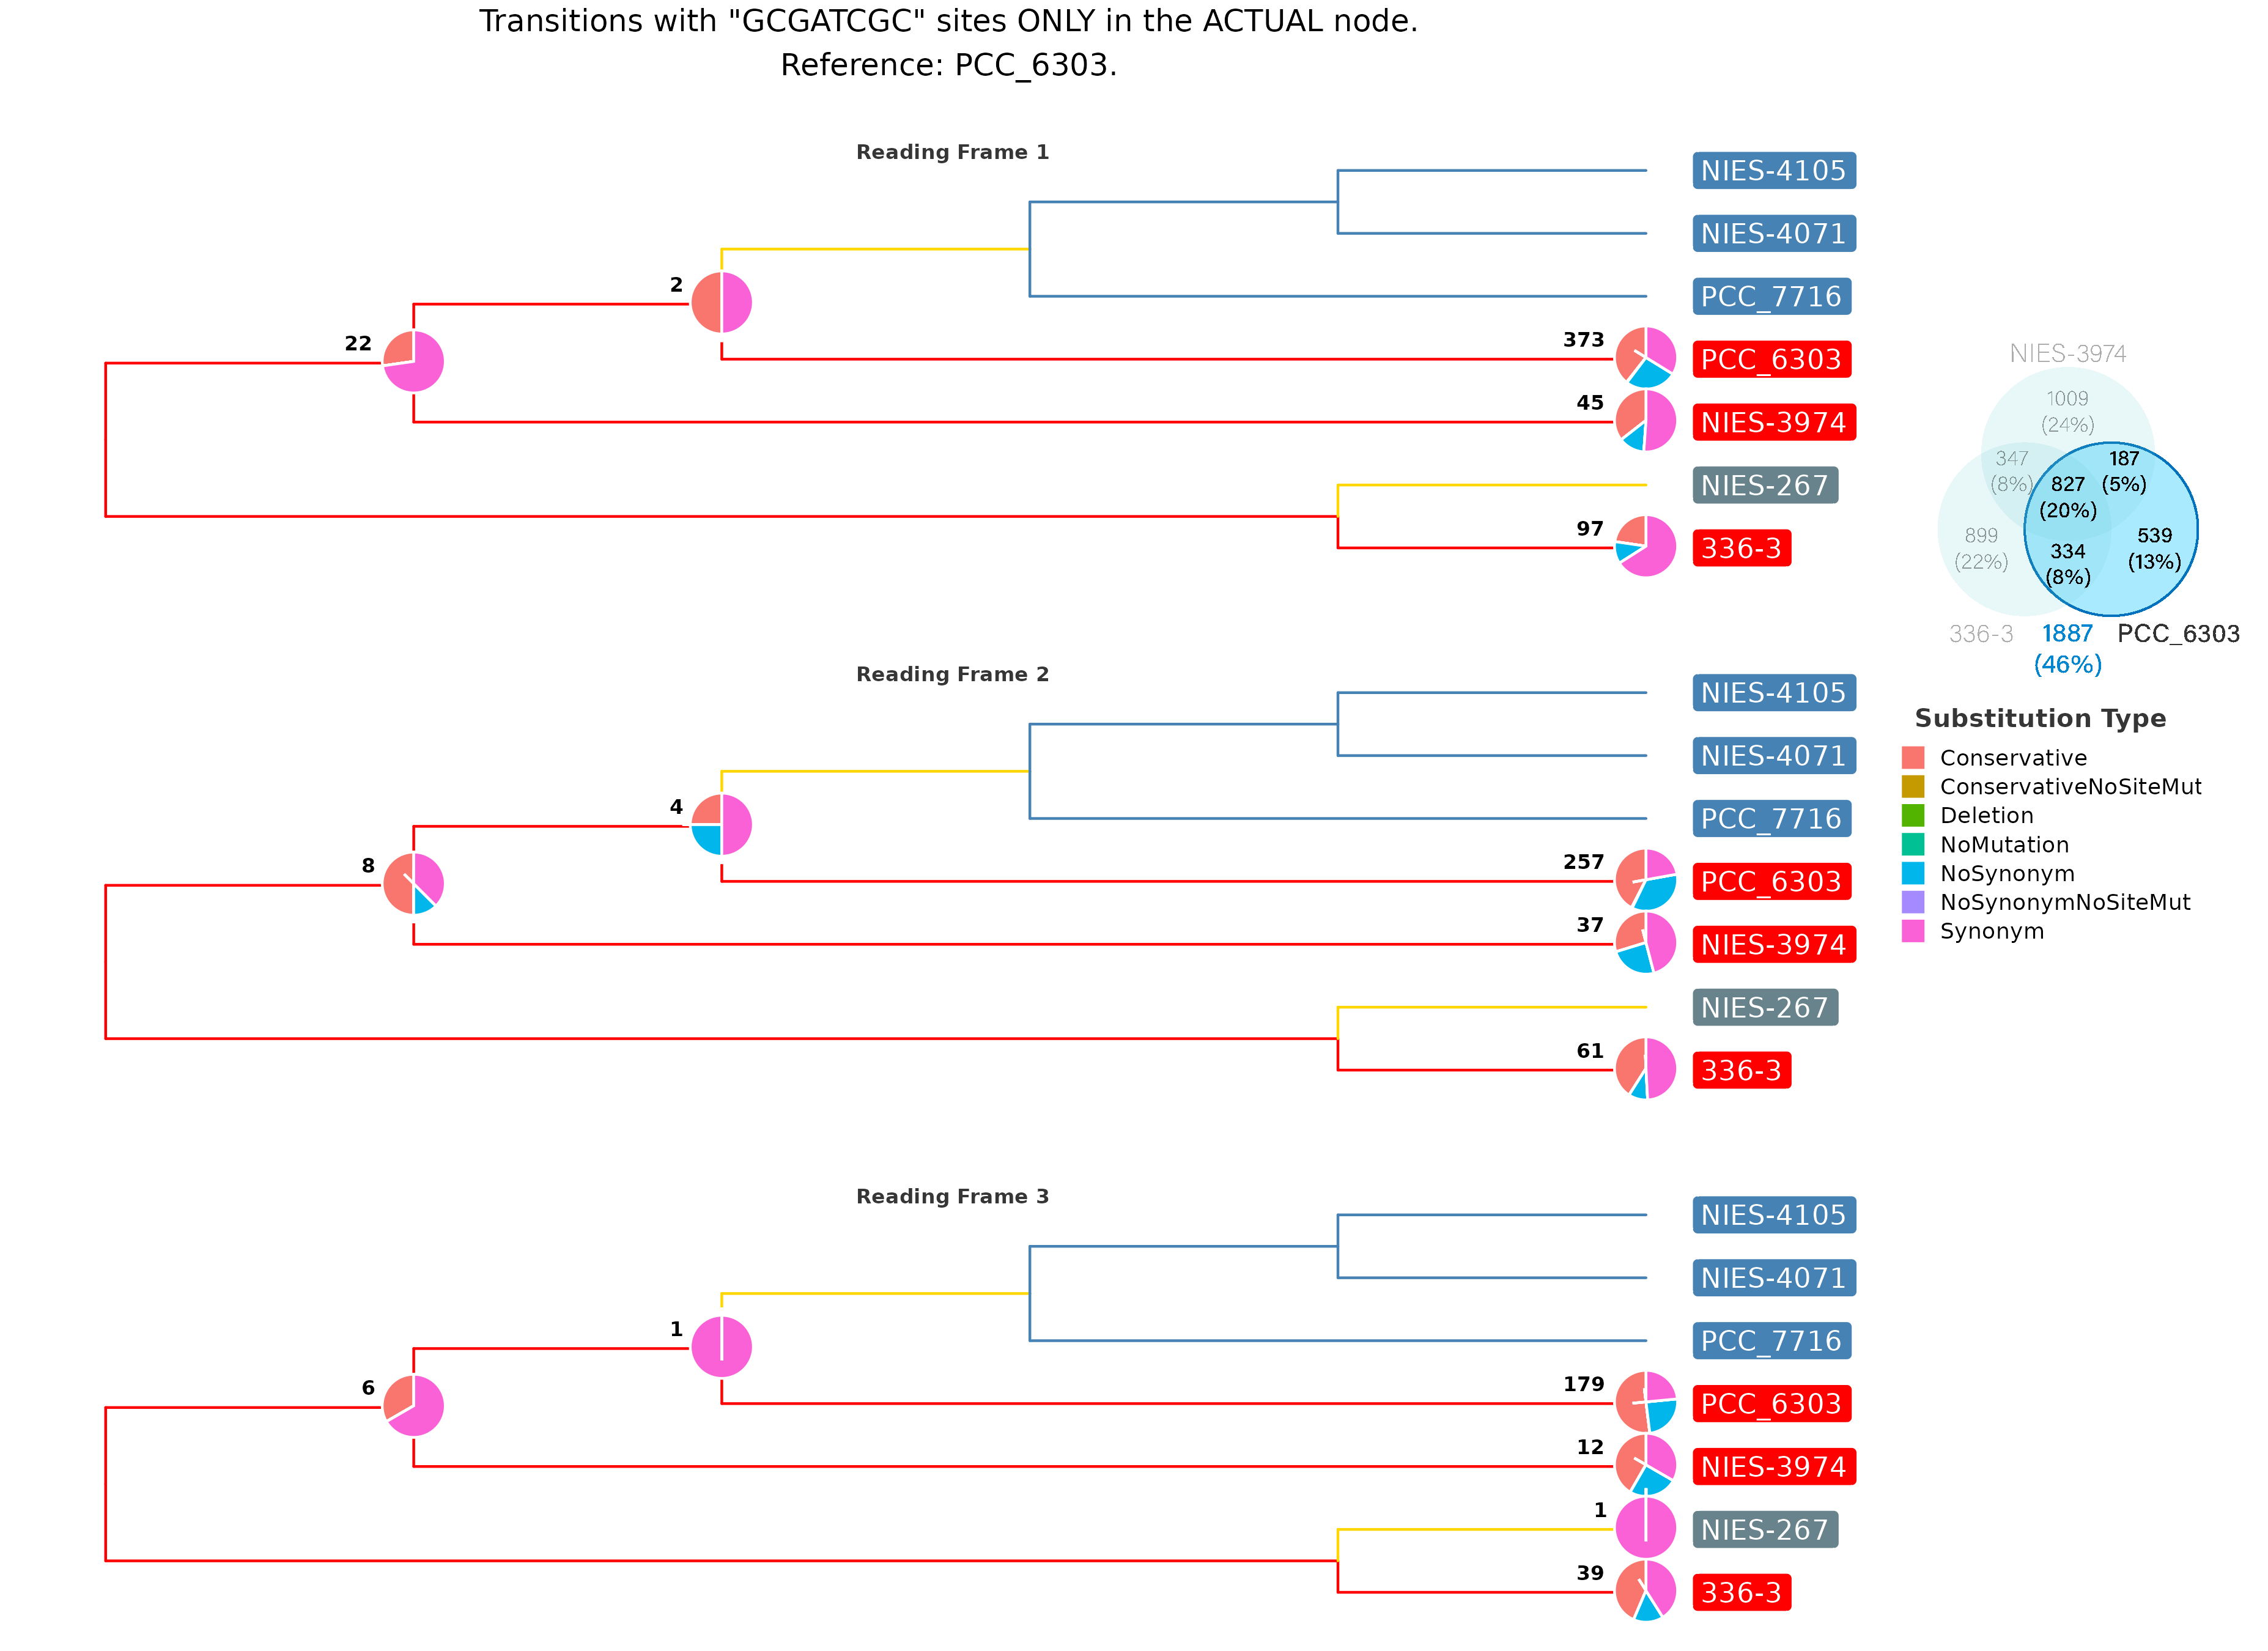
\includegraphics[width=1.2\linewidth]{Clados/Calothrix_B/figures/A/GCGATCGC/Actual/PCC_6303_Actual_A_tree} 

}

\caption{**Conjuntos de sitios de la especie PCC\_6303 en el conjunto ALL.** En esta figura podemos ver la filogenia anotada para los sitios de la especie PCC\_6303, en cada nodo hay un diagrama de pie que muestra la proporcion de tipos de cambios en los aminoacidos que hubo en cada transición. Éstas proporciones se muestran para los tres marcos de lectura.}\label{fig:FIG15}
\end{figure}

\begin{figure}

{\centering 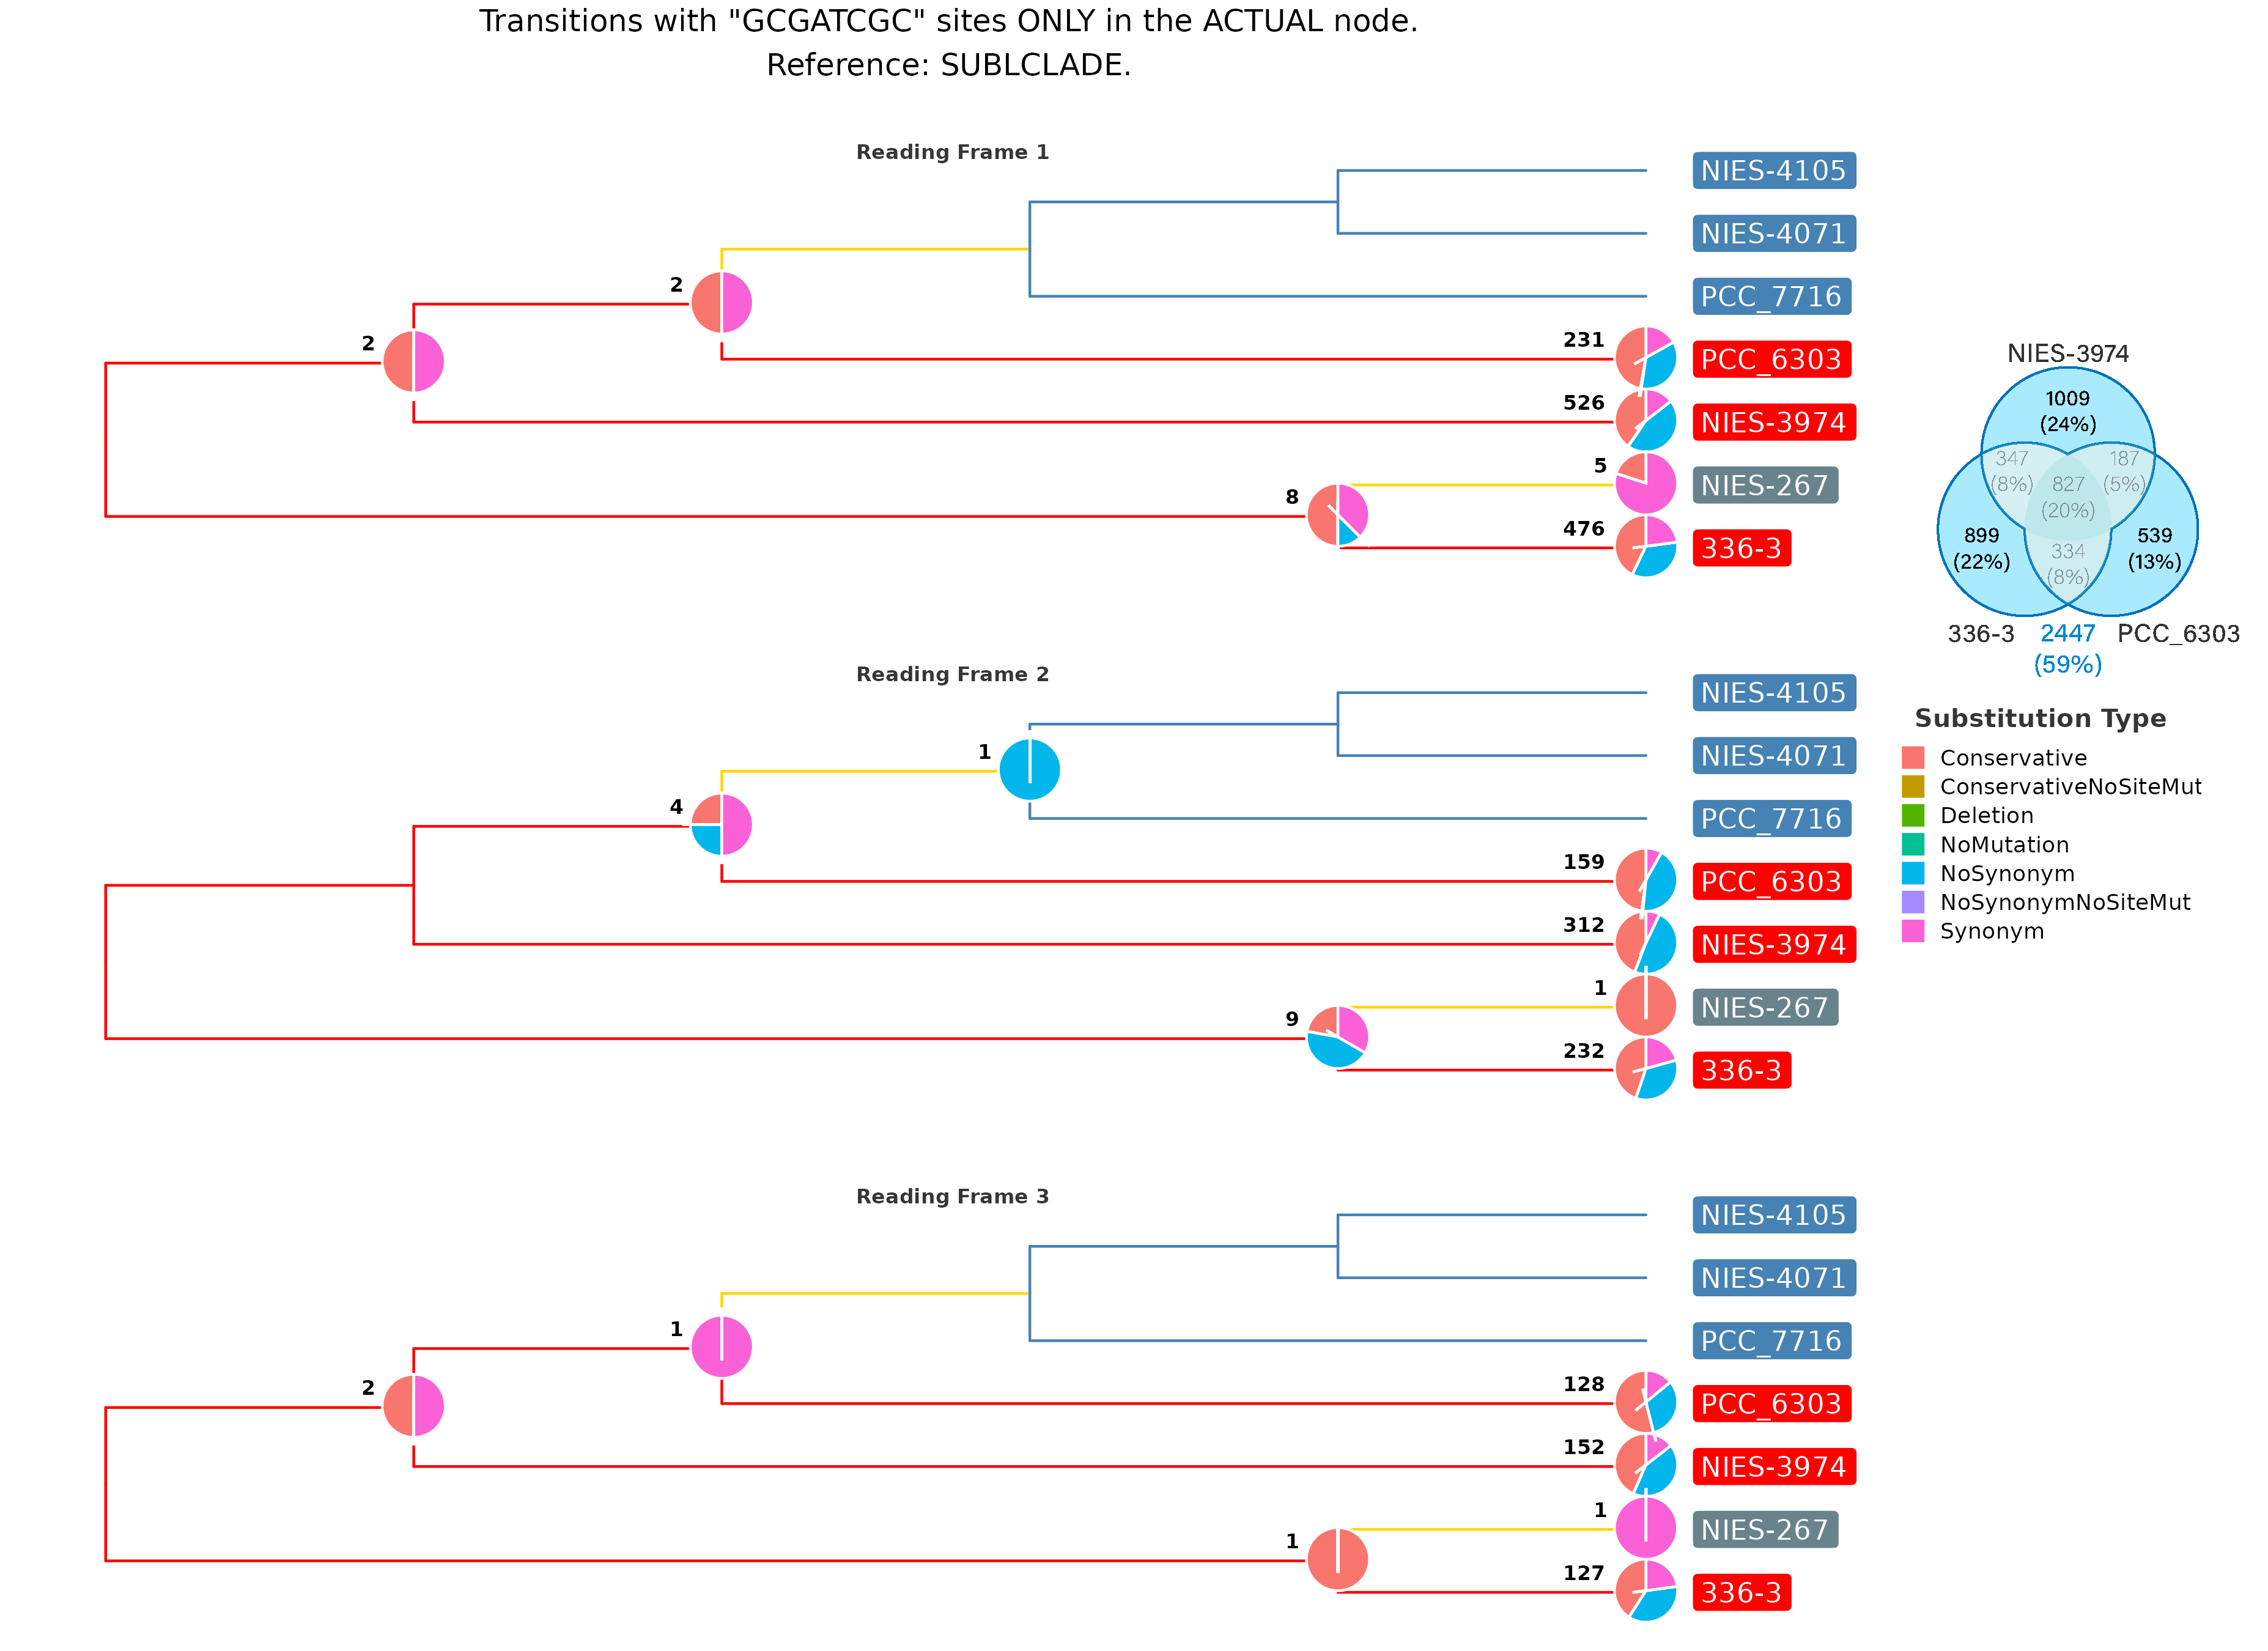
\includegraphics[width=1.2\linewidth]{Clados/Calothrix_B/figures/A/GCGATCGC/Actual/SUBCLADE_Actual_A_tree} 

}

\caption{**Conjuntos de sitios unicos entre las 3 especies en el conjunto ALL.** En esta figura podemos ver la filogenia anotada para todos los sitios unicos entre las 3 especies. En cada nodo hay un diagrama de pie que muestra la proporcion de tipos de cambios en los aminoacidos que hubo en cada transición. Éstas proporciones se muestran para los tres marcos de lectura.}\label{fig:FIG16}
\end{figure}

\hypertarget{tggcgcca}{%
\section{TGGCGCCA}\label{tggcgcca}}

Como se mencionó anteriormente, la importancia del subclado calothrix radica que en 3 de las especies (\textbf{Calothrix PCC 7716}, \textbf{Calothrix sp. NIES 4071} y \textbf{Calothrix sp. NIES 4105}) la abundancia de \textbf{GCGATCGC} es muy baja (o casi nula), además de que contienen otra secuencia palindrómica (\textbf{TGGCGCCA}) la cual tiene abundancia baja (o nula) en las otras tres especies (\textbf{Calothrix sp. 336/3}, \textbf{Calothrix sp. NIES 3974} y \textbf{Calothrix sp. PCC 6303}). Por lo tanto, para ver que estaba sucediendo con esta otra secuencia y si estaba relacionada con \textbf{GCGATCGC}. Realizamos el mismo análisis.

  \bibliography{book.bib,packages.bib}

\end{document}
